% ----------------------------------------------------------------------
%              Latex PhD template for the University of Deusto
% ----------------------------------------------------------------------

\documentclass[twoside,12pt]{Latex/Classes/PhDthesisPSnPDF}

\usepackage{ifthen}
\usepackage{framed}
%\usepackage{slashbox}
\usepackage{arydshln}
\usepackage{comment}

\usepackage{subfigure}
\usepackage{float}
\usepackage[official]{eurosym}
\usepackage{url}

\usepackage[pdftex]{graphicx}
\usepackage{verbatim}
\usepackage{amsmath}

\usepackage{amsfonts}
\usepackage{listings}

\usepackage{algorithm}
\usepackage{algorithmic}

%\ifpdf
%\usepackage{minted}
%\usepackage{multirow}
%\fi

% Test it his works for correct hyphenation
\usepackage[british]{babel}

\usepackage{pifont}
\usepackage{rotating}
\usepackage{multirow}
% For quotes
\usepackage[autostyle]{csquotes} 

%% The amssymb package provides various useful mathematical symbols
\usepackage{amssymb}
%% The amsthm package provides extended theorem environments
\usepackage{amsthm, thmtools}
\theoremstyle{definition}
\newtheorem{defn}{Definition} % definition numbers are dependent on theorem numbers

\theoremstyle{constraint}
\newtheorem{cons}{Constraint} % constraint numbers are dependent on theorem numbers

\theoremstyle{problem}
\newtheorem{problem}{Problem} % constraint numbers are dependent on theorem numbers

\newtheorem*{hypo}{Hypothesis}
\newtheorem*{goal}{Goal}

\newcommand{\Epsilon}{E}
\newcommand{\Tau}{T}
\newcommand{\todo}[1]{\textcolor{red}{@TODO: #1}}

\newcommand{\myfig}[1]{\hbox{Figure \ref{#1}}}
\newcommand{\mytab}[1]{\hbox{Table \ref{#1}}}
\newcommand{\mysec}[1]{\hbox{Section \ref{#1}}}
\newcommand{\mycha}[1]{\hbox{Chapter \ref{#1}}}

\newcommand{\primeraletra}{periodico} % normal, epica, periodico

\ifthenelse{\equal{\primeraletra}{normal}}{
     \newcommand{\letra}[2]{#1#2}
}{
\ifthenelse{\equal{\primeraletra}{epica}}{
    \usepackage{yfonts,color}
    \newcommand{\letra}[2]{\yinipar{\color{red}#1}#2}
}{
\ifthenelse{\equal{\primeraletra}{periodico}}{

    \usepackage{lettrine}
    \newcommand{\letra}[2]{\lettrine[lines=4]{\color{BrickRed}#1}{#2}}
}{
  % TODO ERROR
}
}
}

% Macros help you summarise frequently repeated Latex commands.
% Here, they are placed in an external file /Latex/Macros/MacroFile1.tex
% An macro that you may use frequently is the figuremacro (see introduction.tex)
\include{Latex/Macros/Macros}

\hypersetup{
    colorlinks=false,
    pdfborder={0 0 0},
}

\hyphenation{Deus-to ge-ne-ra-les me-ca-nis-mos mo-de-lar}

%: ----------------------------------------------------------------------
%:                  TITLE PAGE: name, degree,..
% ----------------------------------------------------------------------
% below is to generate the title page with crest and author name

% if output to PDF then put the following in PDF header
\ifpdf  
    \pdfinfo { /Title  (PhD)
               /Creator (TeX)
               /Producer (pdfTeX)
               /Author (Gorka Azkune)
               /CreationDate (D:YYYYMMDDhhmmss)  %format D:YYYYMMDDhhmmss
               /ModDate (D:YYYYMMDDhhmm)
               /Subject (xyz)
               /Keywords (keyword1, keyword2, keyword3) }
    \pdfcatalog { /PageMode (/UseOutlines)
                  /OpenAction (fitbh)  }
\fi


% Title of the dissertation
%\title{Towards Dynamic and Personalised Knowledge-Driven Activity Models}
%\title{Towards a Dynamic and Personalised Hybrid Activity Modelling System}
%\title{Towards Dynamic and Personalised Knowledge-Based Activity Models}
\title{Learning for Dynamic and Personalised Knowledge-Based Activity Models}
%\title{Towards a Dynamic and Personalised Activity Modelling System Combining Knowledge- and Data-Driven Approaches}
%\title{Learning Complete and Specialised Knowledge-Based Activity Models}



% ----------------------------------------------------------------------
% This section below defines front covert (external and internal)
% Shield logo
\crest{\includegraphics[width=2cm]{Deusto_Shield}}
% Full logo
%\crest{\includegraphics[width=6cm]{UDeusto}}
\university{Universidad de Deusto}
\degree{Tesis doctoral presentada por }
\author{Gorka Azkune} 
\collegeordept{dentro del Programa de Doctorado en Ingenier\'ia para la Sociedad de la Informaci\'on y Desarrollo Sostenible}
\textadvisor{Dirigida por }
\advisor{Dr. Diego L\'opez-de-Ipi\~na y Dr. Liming Chen}
\textsignaturecandidate{El doctorando}
\textsignatureadvisor{Los directores}
\cityofbirth{Bilbao}
%\degreedate{\monthname \ \the\year}
\degreedate{Enero de 2015}


% ----------------------------------------------------------------------
       
% turn of those nasty overfull and underfull hboxes
\hbadness=10000
\hfuzz=50pt


%: --------------------------------------------------------------
%:                  FRONT MATTER: dedications, abstract,..
% --------------------------------------------------------------

\begin{document}

\selectlanguage{british}

% sets line spacing: TODO: quitar esto
%\renewcommand\baselinestretch{1.2}
%\baselineskip=18pt plus1pt

% Watermark
%\watermark{DRAFT	DRAFT	DRAFT	DRAFT	DRAFT	DRAFT	DRAFT	DRAFT	DRAFT}


%: ----------------------- generate cover page ------------------------

\maketitle  % command to print the title page with above variables

% Title back
% Thesis Titleback ---------------------------------------------------

\thispagestyle{empty}

\hfill

\vfill

\medskip

\noindent
\textit{
\title
}




Author: Gorka Azkune

Advisor: Dr. Diego L\'opez-de-Ipi\~na

Co-advisor: Dr. Liming Chen

\vfill

\vfill

\noindent
%The following web-page address contains up to date information about this dissertation and related topics: \\
%\url{http://paginaspersonales.deusto.es/porduna/phd/}


\noindent
Text printed in Bilbao

% TODO final date
\noindent
First edition, 
% Moth and year
% \monthname \ \the\year
January\ 2015

\vspace{1cm}
\hrule
\bigskip

% \cleardoublepage command ends the current page and causes all figures and tables that have so far appeared in the input to be printed. In a two-sided printing style, it also makes the next page a right-hand (odd-numbered) page, producing a blank page if necessary. 
\cleardoublepage

%%: ----------------------- cover page back side ------------------------
%% Your research institution may require reviewer names, etc.
%% This cover back side is required by Dresden Med Fac; uncomment if needed.
%
%\newpage
%\vspace{10mm}
%1. Reviewer: Name
%
%\vspace{10mm}
%2. Reviewer: 
%
%\vspace{20mm}
%Day of the defense:
%
%\vspace{20mm}
%\hspace{70mm}Signature from head of PhD committee:
%
%
%\cleardoublepage

% ----------------------------------------------------------------------






%: ----------------------- abstract ------------------------

% Your institution may have specific regulations if you need an abstract and where it is to be placed in the document. The default here is just after title.


% The original template provides and abstractseparate environment, if your institution requires them to be separate. I think it's easier to print the abstract from the complete thesis by restricting printing to the relevant page.
% \begin{abstractseparate}
%   
% Thesis Abstract -----------------------------------------------------


%\begin{abstractslong}    %uncommenting this line, gives a different abstract heading


\begin{abstracts}        %this creates the heading for the abstract page
\selectlanguage{british}
% Put your abstract or summary here.

English abstract here

\end{abstracts}

\begin{resumen}        %this creates the heading for the abstract page
\selectlanguage{spanish}
% Pon tu resumen aquí.

Resumen en espa\~nol aqu\'i


\end{resumen}

\begin{laburpena}        %this creates the heading for the abstract page
 \selectlanguage{basque} 
 % Idatzi hemen zure laburpena
 
 Laburpena euskaraz hemen
 
\end{laburpena}



%\end{abstractlongs}


% ---------------------------------------------------------------------- 

% \end{abstractseparate}


%: ----------------------- tie in front matter ------------------------

% The frontmatter text starts here
\frontmatter

% Thesis Dedictation ---------------------------------------------------

\begin{dedication} %this creates the heading for the dedication page

\textit{Ama eta Nagoreri}

\end{dedication}

% ----------------------------------------------------------------------



% Thesis Abstract -----------------------------------------------------


%\begin{abstractslong}    %uncommenting this line, gives a different abstract heading


\begin{abstracts}        %this creates the heading for the abstract page
\selectlanguage{british}
% Put your abstract or summary here.

English abstract here

\end{abstracts}

\begin{resumen}        %this creates the heading for the abstract page
\selectlanguage{spanish}
% Pon tu resumen aquí.

Resumen en espa\~nol aqu\'i


\end{resumen}

\begin{laburpena}        %this creates the heading for the abstract page
 \selectlanguage{basque} 
 % Idatzi hemen zure laburpena
 
 Laburpena euskaraz hemen
 
\end{laburpena}



%\end{abstractlongs}


% ---------------------------------------------------------------------- 


% Thesis Acknowledgements ------------------------------------------------


% Opening of the acknowledgements

%Sort version
%this creates the heading for the acknowlegments
\begin{acknowledgements}      
%Long version
%uncommenting this line, gives a different acknowledgements heading
%\begin{acknowledgementslong} 
Even though science aims at overcoming human biases and irrational behaviours, science is done by scientists. And scientists, in the end of the day, are human. Humans tend to feel gratitude for those who help them pursuing an objective. I am not an exception. I think it is very important to express that gratitude, because without the help and support of several people, this PhD dissertation would not have been possible. Thus, my objective, my dream, would only exist in my mind.

Lo primero de todo es agradecer a Diego: has creído en mí y has puesto toda la carne en el asador para que se pueda realizar esta tesis doctoral tal y como habíamos previsto. Después de muchos años, has conseguido que me sienta un investigador de nuevo. 

It is also very important for me to thank Luke. Your research work inspired many of the ideas of this dissertation and I was lucky enough to get you on board. It is not only about your technical support and guidance, but also about your kindness. It has been a pleasure to work with you.

La persona que más ha tenido que soportarme ha sido sin duda Aitor. Desde el primer día me has ayudado mucho. Hemos tenido muchas reuniones y discusiones donde esta tesis ha ido cogiendo forma. Has revisado todo mi trabajo, nuestras publicaciones y me has echado una mano con la burocracia interna que siempre tanto me cuesta. Por todo ello, muchísimas gracias.

No podría olvidarme tampoco de todos los compañeros del laboratorio. Además de acogerme tan bien, os agradezco el esfuerzo que dedicasteis a la evaluación de esta tesis. Toda la información que me disteis ha sido clave para poder validar todo mi trabajo.

Tesi hau, beste gauza guztien gainetik, nire amarentzat omenaldi xume bat da. Badakit zuretzat berandu iritsi dela, ezin duzula gustatuko litzaizukeen bezala disfrutatu, baina oraindik badut esperantza zure buru barruan, txokoren batean eta momenturen batean, zure semeaz harro sentituko zarela.


\begin{flushright}
\textit{Eskerrik asko,}

Gorka Azkune

% Moth and year
December 2014
%\monthname \ \the\year



% Signature figure

%\begin{figure}[htbp!]
%\end{figure}
%\includegraphics{signature}%



\end{flushright}



%Closing of the acknowledgements
%Sort version
\end{acknowledgements}
% Long version
%\end{acknowledgementslong}

% ------------------------------------------------------------------------




% As abstract contains various languages we set the main language again
\selectlanguage{british}


%: ----------------------- contents ------------------------

\setcounter{secnumdepth}{5} % organisational level that receives a numbers
\setcounter{tocdepth}{5}    % print table of contents for level 3


%%You can also add extra lines to the ToC or to force extra unnumbered section headings to be included. For example, if you wanted to add an entry called Preface, and you didn't want the Preface to be numbered, you'd use these commands:
%\ subsection*{Preface}
%\addcontentsline{toc}{subsection}{Preface} 

\tableofcontents            % print the table of contents
% levels are: 0 - chapter, 1 - section, 2 - subsection, 3 - subsection

%: ----------------------- list of figures/tables ------------------------

\listoffigures	% print list of figures
\listoftables  % print list of tables
\renewcommand{\listtheoremname}{List of definitions}
\listoftheorems[ignoreall, show={defn}]
%\listoftheorems[show={defn}]

%: ----------------------- glossary ------------------------

% Tie in external source file for definitions: /0_frontmatter/glossary.tex
% Glossary entries can also be defined in the main text. See glossary.tex

% this file is called up by thesis.tex
% content in this file will be fed into the main document

% Glossary entries are defined with the command \nomenclature{1}{2}
% 1 = Entry name, e.g. abbreviation; 2 = Explanation
% You can place all explanations in this separate file or declare them in the middle of the text. Either way they will be collected in the glossary.

% required to print nomenclature name to page header
\markboth{\MakeUppercase{\nomname}}{\MakeUppercase{\nomname}}

% ----------------------- contents from here ------------------------
%

%
%
%% acronyms

\nomenclature{API}{Application Programming Interface}
\nomenclature{AJAX}{Asynchronous JavaScript And XML}
\nomenclature{CMS}{Content Management System}
\nomenclature{CPLD}{Complex Programmable Logic Device}
\nomenclature{FPGA}{Field Programmable Gate Array}
\nomenclature{GNU}{GNU's Not Unix}
\nomenclature{GOLC}{Global Online Laboratory Consortium}
\nomenclature{HTML}{Hyper Text Markup Language}
\nomenclature{HTTP}{Hyper Text Transfer Protocol}
\nomenclature{ID}{Identifier}
\nomenclature{IEEE}{Institute of Electrical and Electronics Engineers}
\nomenclature{IO}{Input/Output}
\nomenclature{IP}{Internet Protocol}
\nomenclature{ISA}{iLab Shared Architecture}
\nomenclature{JSON}{JavaScript Object Notation}
\nomenclature{LMS}{Learning Management System}
\nomenclature{MIT}{Massachusetts Institute of Technology}
\nomenclature{MOOC}{Massive Open Online Courses}
\nomenclature{ORM}{Object-Relational Mapping}
\nomenclature{RDP}{Remote Desktop Protocol}
\nomenclature{RLMS}{Remote Laboratory Management System}
\nomenclature{RPC}{Remote Procedure Call}
\nomenclature{SOAP}{Simple Object Access Protocol}
\nomenclature{SPRL}{Single Purpose Remote Laboratory}
\nomenclature{SQL}{Structured Query Language}
\nomenclature{SSH}{Secure SHell}
\nomenclature{STEM}{Science, Technology, Engineering and Mathematics}
\nomenclature{TEL}{Technology-Enhanced Learning}
\nomenclature{UML}{Unified Modelling Language}
\nomenclature{UNED}{Universidad Nacional de Education a Distancia}
\nomenclature{UTS}{University of Technology, Sydney}
\nomenclature{VISIR}{Virtual Instrumentation Systems In Reality}
\nomenclature{VHDL}{VHSIC Hardware Description Language}
\nomenclature{VHSIC}{Very-High-Speed Integrated Circuits}
\nomenclature{VM}{Virtual Machine}
\nomenclature{VNC}{Virtual Network Computing}
\nomenclature{WSDL}{Web Service Description Language}
\nomenclature{XML}{eXtensible Markup Language}




%\begin{multicols}{2} % \begin{multicols}{#columns}[header text][space]
%\begin{footnotesize} % scriptsize(7) < footnotesize(8) < small (9) < normal (10)

%\printnomenclature[1.5cm] % [] = distance between entry and description

\printnomenclature[1.5cm] % [] = distance between entry and description

\label{sec:glossary} % target name for links to glossary

%\end{footnotesize}
%\end{multicols}




%: --------------------------------------------------------------
%:                  MAIN DOCUMENT SECTION
% --------------------------------------------------------------

% the main text starts here with the introduction, 1st chapter,...
\mainmatter

%\renewcommand{\chaptername}{} % uncomment to print only "1" not "Chapter 1"
\pagestyle{fancy}

%: ----------------------- subdocuments ------------------------

% Parts of the thesis are included below. Rename the files as required.
% But take care that the paths match. You can also change the order of appearance by moving the include commands.

%: ----------------------- introduction ------------------------


% this file is called up by thesis.tex
% content in this file will be fed into the main document

%: ----------------------- introduction file header -----------------------
\begin{savequote}[50mm]
Science is a way of trying not to fool yourself. The first principle is that you must not fool yourself, and you are the easiest person to fool.
\qauthor{Richard Feynman}
\end{savequote}


\chapter{Evaluation}
\label{cha:evaluation}

% the code below specifies where the figures are stored
\ifpdf
    \graphicspath{{6_evaluation/figures/PDF/}{6_evaluation/figures/PNG/}{6_evaluation/figures/}}
\else
    \graphicspath{{6_evaluation/figures/EPS/}{6_evaluation/figures/}}
\fi

\letra{T}{his} chapter describes and analyses the proposed evaluation methodology for the extended activity model learning system described through Chapters \ref{cha:archi}, \ref{cha:clustering} and \ref{cha:learner}. To test the learning system properly, detailed data from various users is needed, containing different ways of performing the same activity by the same user. In order to achieve such datasets, the proposed evaluation methodology is based on surveys to users and a synthetic dataset generator tool. Surveys allow capturing how users perform activities in terms of actions, while the synthetic dataset generator uses survey information to generate sensor activation datasets, introducing different kinds of sensor noise. 

Once the methodology is described and discussed, evaluation scenarios and metrics will be introduced. To assess the performance of the learning system in various situations, several evaluation scenarios have been prepared, considering different kinds of sensor noise and set-ups. Similarly, and based on the available literature, the most significant performance metrics have been chosen to measure the performance of the approach.

Applying the evaluation methodology on the prepared scenarios and selected metrics, results are obtained. Those results are widely discussed in this chapter and compared to the objectives defined in Chapter \ref{cha:introduction}.

The chapter is divided in three sections: Section \ref{sec:evaluation:methodology} introduces the conventional evaluation methodology used for activity recognition, detects its drawbacks and proposes a new evaluation methodology which is more appropriate to validate the learning system. Section \ref{sec:evaluation:scenarios} presents evaluation scenarios, metrics, results and discussions divided in three main parts: $SA³$ performance (Section \ref{subsec:evaluation:sa3}), the complete activity clustering performance (Section \ref{subsec:evaluation:clustering}) and finally the EAM learning system performance (Section \ref{subsec:evaluation:eam}). All three sections discuss the results and compare them with the objectives identified at the beginning of this dissertation (Chapter \ref{cha:introduction}). To conclude, Section \ref{sec:evaluation:conclusions} provides a global view of the system performance, summarises the contents of the chapter and presents the most relevant conclusions.
\section{Context and Motivation}
\label{sec:intro:context}

%Describe the context of activity recognition, enhancing why it is needed and how it has been approached. Explain briefly how knowledge-driven systems work and which are their drawbacks to claim that this dissertation aims at overcoming one of those drawbacks: static activity models.

% Distinguish between activity modelling and recognition; Modelling is not an one-off activity but an iterative multi-phase process; Modelling and recognition are interweaved, both improved incrementally; Add an image where this cycle is shown (Chen's presentation)

Independently from the approach used to implement activity recognition systems, it is usually the case where activity modelling and recognition are carried out separately. Activity modelling is very important for activity recognition, since it provides the models which have to be recognised in the sensor datasets generated by humans while they perform activities. While data-driven approaches obtain those models directly from user generated data, knowledge-driven approaches obtain them by means of knowledge engineering techniques. However, both approaches share usually the same assumption, i.e. activity modelling is performed once and afterwards, the generated models are used for activity recognition. 

% People tend to change the way they perform activities, executing different action sequences for the same activities; this is specially true for elderly people, whose cognitive impairments may be associated with their habit changes

Assuming the static nature of activity models does not fit to the reality. People tend to change the way they perform the same activities in time. Hence, the same activity models cannot be used forever. From the point of view of data-driven activity modelling approaches, implementing dynamic activity models is not a problem, as incremental learning techniques can be used \cite{Rashidi2011}. Moreover, as activity models are learned directly from user generated data, personalised activity models are naturally obtained. Two of the positive features of data-driven modelling are thus dynamic and personalised models. But those virtues pose also some drawbacks: activity models are not generic so they cannot be applied to other users and activity models are usually incomprehensible for humans which make their usage for other applications much harder.

% Talk about knowledge-driven approaches and show how the activity models obtained by knowledge engineering techniques are usually static; focus specially on actions, which are the key elements for recognition

On the other hand, knowledge-driven modelling produces generic and human understandable models, since activities are modelled by their intrinsic features and relations rather than from data, and activity models are expressed using logical and descriptive formalisms \cite{Chen2012a}. However, those models are usually static, i.e. once they have been defined they do not evolve. In addition to it, obtaining personalised models is very complicated because experts cannot know in advance all the personal features of a concrete user. 

% To have dynamic knowledge-driven activity modelling, a new process is proposed: (i) domain experts provide initial activity models, (ii) inhabitants produce sensor datasets while performing activities, (iii) a learning system improves the initial activity models and presents them to the domain expert, (iv) domain expert validates models and adds them to the knowledge base

It is quite clear then that both activity modelling approaches have complementary advantages and disadvantages. An approach excels where the other fails. It seems natural thus to try to combine both approaches in order to develop a better activity modelling process where generic and personalised models can be obtained and those models evolve in time with user generated data. 

\begin{figure}[htbp]
\centering
\includegraphics[width=\textwidth]{activity_modelling.pdf}
    \caption{The continuous activity model process to obtain dynamic and personalised models from generic expert provided models.}
    \label{fig-activity-modelling}
\end{figure}

In this dissertation, a continuous activity modelling process is presented, where domain experts provide initially generic activity models using knowledge engineering tools, to afterwards run data-driven learning algorithms on user generated data to learn personalised models. Such personalised models will be presented to the expert, who can add or update them in the knowledge base. This loop is continuously repeated in time to achieve dynamic and personalised models based on initially provided generic models and user generated data. Figure \ref{fig-activity-modelling} shows a diagram with the described process.

The described activity modelling process uses generic knowledge-driven activity models provided by a domain expert, achieving thus generic and understandable activity models. To solve the problem of personalised models, user generated data is used in a learning process to produce knowledge-driven personalised models. This means that data-driven learning techniques are used to capture personal features of generic activities and obtain understandable personalised activity models. Such models, after expert validation, are added to the knowledge base to use them subsequently in activity recognition systems. Repeating this process continuously, dynamic activity models are obtained, which evolve in time as users change - or not - their habits.

% One of the key elements of this process is the learning system, which has to learn new actions for already defined activities -> this is the target of the thesis; provide an example (MakeCoffee) with its image

When modelling activities, two major aspects are considered: the actions carried out to perform the activity and the descriptive features of the activity \cite{Chen2014}. Actions refer to object interactions. For example, to prepare a coffee a user might have coffee and a cup to drink the coffee. This sequence can be modelled as the action sequence of \textit{hasCoffee} and \textit{hasContainer}, which are obtained from the interactions with the respective objects monitored by sensors. Descriptive properties of an activity refer to the time when the activity has been performed, its duration, the concrete set of objects used and their order. Both aspects of an activity model, i.e. actions and descriptive properties, may vary from person to person. 

As far as learning personalised descriptive properties for knowledge-driven models regards, Chen et al. already combined data-driven and knowledge-driven approaches in \cite{Chen2014}. However, to the best of our knowledge, a similar work to learn specific actions for activity models has not been published yet. In fact, Chen et al. assume in their work that the actions in the \textit{seed} activity models provided by domain experts can be used for any user. This means that every user has to execute the same actions to perform a concrete activity.

In this dissertation, the problem of learning actions for given activities is analysed. It cannot be generally assumed that every user executes the same actions to perform a concrete activity. Imagine, for instance, that a user prepares a coffee and adds sugar to it. To make it simple, the activity model for this user could contain the actions \textit{hasCoffee}, \textit{hasContainer}, \textit{hasWater} and \textit{hasFlavour}. But there is another user who does not like any flavourant, so she prepares coffee by means of actions \textit{hasCoffee}, \textit{hasContainer} and  \textit{hasWater}. As it can be seen, both activity models are different as far as actions regard, but both of them are valid models for the activity of making a coffee. 

To develop a proper activity modelling process, learning actions is a key feature. It has been observed that generic activity models provided by a domain expert have the necessary actions to perform an activity, but not sufficient actions for personalised models. Those activity models can be used to further learn new actions for different users and thus generate new personalised activity models. Let us illustrate our hybrid activity modelling approach with an example. Figure \ref{fig-objective} shows an initial generic activity model for the MakeCoffee activity, which is composed by the actions \textit{hasCoffee} and \textit{hasContainer}. These are the necessary actions for every person to perform a MakeCoffee activity, which highlight the indispensable actions of making a coffee, i.e. the use of coffee and a container to place the coffee in. Nevertheless, some users might add some milk and sugar, others cream etc. The idea of our approach is to create high-level activity models with only these indispensable actions - generic models -, and then use the data generated by a specific user performing the activity to learn those new actions which also configure the personal way of making coffee. In the case of Figure \ref{fig-objective}, where the initial activity model will only include coffee and container, the system would learn that MakeCoffee is performed in two ways by the user: in the first one, the user adds milk (\textit{hasMilk}) and sugar (\textit{hasFlavour}), while in the second one only sugar is added (\textit{hasFlavour}). Hence two specialised and complete activity models of MakeCoffee can be learned. This way, experts, initially, only have to provide generic but incomplete activity models with necessary actions. Afterwards the learning system can analyse a user's behavioural data and learn the specialised and complete models to enrich the knowledge base, thus improving initial activity models.

Running the proposed learning process periodically with new data generated by a concrete user, a dynamic activity modelling system is achieved. As a user evolves regarding the way she performs certain activities, the learning approach learns new versions of the initial activity models. Hence, activity models can be adapted to users' varying behaviours.

\begin{figure}[htbp]
\centering
\includegraphics[width=9cm]{objective.pdf}
    \caption{Illustrative example of the objective of the dissertation: using the initial incomplete model for MakeCoffee and user generated data, the learning algorithm learns 2 specialised and complete models.}
    \label{fig-objective}
\end{figure}

Notice that the proposed modelling approach does not only learn new actions for initial activity models, but it also learns sub-activities of already defined activities. In the example depicted in Figure \ref{fig-objective}, the two specialised models are two sub-activities of the MakeCoffee activity, namely MakeBlackCoffee and MakeCoffeeWithMilk. This feature makes possible for the expert to define activities in a higher level of abstraction and let the system learn different sub-activities to generate specialised knowledge. 

As a summary, this dissertation is focused on making another step towards dynamic and personalised activity models for knowledge-driven activity recognition systems. A learning system to obtain complete and specialised activity models from generic but incomplete expert provided models has been developed. This step allows implementing activity modelling approaches that use expert knowledge to have generic activity models applicable to every user, and learn new actions for concrete users achieving personalised and dynamic activity models. 
%\section{Motivation}
\label{sec:intro:motivation}

Why is this dissertation interesting? Justify it.


\section{Hypothesis, Objectives and Limitations}
\label{sec:intro:hypothesis}

Write the hypothesis.

Decompose hypothesis in smaller goals and objectives.

Describe constraints and limitations.



\section{Methodology}

A research strategy has been defined in order to achieve the statement presented
above. The strategy is defined as follows:

\begin{enumerate}
    \item Update knowledge by reviewing the literature in the area of activity recognition, knowledge engineering, machine learning and data mining. This analysis has been reinforced by attending specialised scientific conferences.
    \item Critically evaluate existing activity modelling and recognition solutions, analysing their scope and limitations and identifying weak areas where contributions to the state of the art can be done.
    \item Design and develop the different modules of the activity model learner, incrementally adopting more complex and efficient solutions.
    \item Test developed modules through experiments and analyse results to enhance the performance of the system.
    \item Attend conferences and workshops to present partial results and validate them with the scientific community.
    \item Experimentation and evaluation of the prototype at each particular
    stage.
    \item Network with experts at conferences, project meetings and e-mail.
    \item Redesign the activity model learner system with feedback from all this network, as well as the literature.
    \item Select an appropriate evaluation methodology and evaluate consequently the activity model learner system.
    \item Dissemination of the results obtained during the research process.
\end{enumerate}

This methodology is illustrated in \myfig{fig:methodology}.
\InsertFig{Methodology}{fig:methodology}{Methodology used during the
dissertation}{}{0.9}{}

\section{Contributions}
\label{sec:intro:contributions}

The following major and minor contributions can be found in this dissertation:
\begin{itemize}
    \item Contribution and its location in the document.    
\end{itemize}

\section{Thesis Outline}
\label{sec:intro:outline}

The thesis is structured in seven chapters.

Chapter \ref{cha:introduction} is the current chapter. It presents the context and motivation of the research, as well as the hypothesis, goals and scope. To achieve those goals and validate the hypothesis, a research methodology is proposed. Finally, the contributions of the dissertation and their location in the document are also shown.

Chapter \ref{cha:soa} describes the state of the art relevant to the dissertation. The most important activity monitoring, modelling and recognition approaches are presented providing a well structured taxonomy. The chapter also shows the position in such taxonomy of the research performed in this dissertation.

Chapter \ref{cha:archi} establishes the basis of the dissertation, giving a high-level view of the whole system. First of all, the chapter describes in detail ontology-based activity modelling approaches, which serve as reference for the work carried out in this dissertation. Afterwards, a set of definitions and constraints is posed to establish the scope of the research clearly. The knowledge representation formalism and structures are presented and the input data of the system is identified. Finally, the intuition behind the learning system and a high-level design are described.

Chapter \ref{cha:clustering} describes the proposed activity clustering algorithm, which is divided into two main steps: initialisation and action aggregation. Both steps are described in detail, providing pseudo-code for their implementation.

Chapter \ref{cha:learner} explains the last stage of the learning process. Design decisions are explained and a rigorous analysis of all available information to learn activity models is done. The learning algorithm's steps are described in detail and pseudo-code for its implementation is provided.

Chapter \ref{cha:evaluation} evaluates the complete learning system and its constituent parts. For this purpose, the most relevant evaluation methodologies for activity recognition systems are shown and their suitability to evaluate the learning system is analysed. The chapter proposes a new hybrid evaluation methodology, based on surveys to users and simulation tools. Afterwards, evaluation scenarios and metrics are presented and obtained results are shown, leading to a discussion of the learning system, its advantages and drawbacks.

Finally, Chapter \ref{cha:conclusions} summarises the dissertation, draws the conclusions of this research work and shows the related future lines of work.


%: ----------------------- related work ------------------------


% this file is called up by thesis.tex
% content in this file will be fed into the main document

%: ----------------------- introduction file header -----------------------
\begin{savequote}[50mm]
Science is a way of trying not to fool yourself. The first principle is that you must not fool yourself, and you are the easiest person to fool.
\qauthor{Richard Feynman}
\end{savequote}


\chapter{Evaluation}
\label{cha:evaluation}

% the code below specifies where the figures are stored
\ifpdf
    \graphicspath{{6_evaluation/figures/PDF/}{6_evaluation/figures/PNG/}{6_evaluation/figures/}}
\else
    \graphicspath{{6_evaluation/figures/EPS/}{6_evaluation/figures/}}
\fi

\letra{T}{his} chapter describes and analyses the proposed evaluation methodology for the extended activity model learning system described through Chapters \ref{cha:archi}, \ref{cha:clustering} and \ref{cha:learner}. To test the learning system properly, detailed data from various users is needed, containing different ways of performing the same activity by the same user. In order to achieve such datasets, the proposed evaluation methodology is based on surveys to users and a synthetic dataset generator tool. Surveys allow capturing how users perform activities in terms of actions, while the synthetic dataset generator uses survey information to generate sensor activation datasets, introducing different kinds of sensor noise. 

Once the methodology is described and discussed, evaluation scenarios and metrics will be introduced. To assess the performance of the learning system in various situations, several evaluation scenarios have been prepared, considering different kinds of sensor noise and set-ups. Similarly, and based on the available literature, the most significant performance metrics have been chosen to measure the performance of the approach.

Applying the evaluation methodology on the prepared scenarios and selected metrics, results are obtained. Those results are widely discussed in this chapter and compared to the objectives defined in Chapter \ref{cha:introduction}.

The chapter is divided in three sections: Section \ref{sec:evaluation:methodology} introduces the conventional evaluation methodology used for activity recognition, detects its drawbacks and proposes a new evaluation methodology which is more appropriate to validate the learning system. Section \ref{sec:evaluation:scenarios} presents evaluation scenarios, metrics, results and discussions divided in three main parts: $SA³$ performance (Section \ref{subsec:evaluation:sa3}), the complete activity clustering performance (Section \ref{subsec:evaluation:clustering}) and finally the EAM learning system performance (Section \ref{subsec:evaluation:eam}). All three sections discuss the results and compare them with the objectives identified at the beginning of this dissertation (Chapter \ref{cha:introduction}). To conclude, Section \ref{sec:evaluation:conclusions} provides a global view of the system performance, summarises the contents of the chapter and presents the most relevant conclusions.
\section{Human Activity Recognition}
\label{sec:soa:har}

%Talk about human activity recognition as a research topic. Explain in what application it has been used, how and for what and different sensor approaches used. Make clear that this dissertation will be based on sensor-based activity recognition.

Human activity recognition has become a key research topic in diverse areas, including pervasive and mobile computing \cite{Weiser1991} \cite{Choudhury2008}, surveillance-based security \cite{Poppe2010} \cite{Akdemir2008} \cite{Weinland2011}, context-aware computing \cite{Laerhoven2001} \cite{Wren2006}, ambient assisted living \cite{Philipose2004} \cite{Cook2009} \cite{Kasteren2008} \cite{Chen2012a} and social robotics \cite{Fong2003a} (my JINT paper?). The interest in activity recognition has recently increased attributing to the intensive thrusts from the latest technology development and application demands. The progress in sensor technologies has been substantial over the past decade, especially low-power, low-cost, high-capacity and miniaturised sensors, wired and wireless communication networks \cite{Pantelopoulos2010} \cite{Alemdar2010} \cite{Ding2011}. In parallel, data processing techniques have also shown important advances, based on higher computational capabilities of devices and the development of novel algorithms. The progress and maturity of these supporting technologies have pushed the research focuses of the aforementioned areas to shift from low-level data collection and transmission towards high-level information integration, context processing and activity recognition and inference. At the same time, activity recognition has been demanded by a growing number of solutions for real-world problems and applications. For example, surveillance and security try to make use of activity recognition technologies to address the threats of terrorists. Ambient assisted living aims to exploit activity monitoring, recognition and assistance to support independent living and ageing in place. Other emerging applications, such as intelligent meeting rooms and smart hospitals, are also dependent on activity recognition in order to provide multimodal interactions, proactive service provision, and context aware personalised activity assistance. 

As a result of the technology push and application pull, activity recognition has built its own space in the academic world. As such, research related to activity recognition has become regular topics in mainstream international conferences in related areas such as the AAAI Conference on Artificial Intelligence\footnote{http://www.aaai.org/}, Computer Vision and Pattern Recognition\footnote{http://www.cvpr201x.org/}, International Joint Conference on Artificial Intelligence\footnote{http://ijcai.org/}, International Joint Conference on Pervasive and Ubiquitous Computing\footnote{http://ubicomp.org/}, International Conference on Pervasive Computing and Communications\footnote{http://www.percom.org/} and International Joint Conferences on Ambient Intelligence\footnote{http://www.ami-conferences.org/}. In order to try to channel the research towards future applications, a substantial number of projects and initiatives have been undertaken. Good examples are \textit{The Ambient Assisted Living Joint Programme}\footnote{www.aal-europe.eu}, \textit{The House of the Future}\footnote{http://architecture.mit.edu/house\_n}, \textit{The Gator-Tech Smart House}\footnote{http://www.icta.ufl.edu/gt.htm} or \textit{The iDorm project}\footnote{http://cswww.essex.ac.uk/iieg/idorm.htm}.  %In addition, a growing number of workshops have been dedicated to activity recognition research from different research angles and communities. For example, in 2011 alone eight workshops were specifically devoted to activity recognition research, including IWFAR [24], HAU3D [25], SAGAware [26], PAIR [27], GAPRec [28] and others [29][30][31]. The interest and enthusiasm for this topic is still increasing.

Apart from potential applications, activity recognition has gained research interest because it is a multidisciplinary and complex process. Activity recognition can be roughly characterized by four basic tasks. These tasks include:
\begin{enumerate}
 \item Selection and deployment of appropriate sensors to objects and environments in order to monitor and capture a user’s behaviour along with the state change of the environment.
 \item To collect, store and process perceived information through data analysis techniques and/or knowledge representation formalisms at appropriate levels of abstraction.
 \item To create computational activity models in a way that allows software systems/agents to conduct reasoning and manipulation.
 \item To select or develop reasoning algorithms to infer activities from sensor data.
\end{enumerate}

Each individual task can be tackled by a great variety of methods, technologies and tools. It is often the case that the selection of a method used for one task is dependent on the method of another task. As such, activity recognition has been classified in the following ways. The first classification criterion focuses on the sensors used for activity monitoring, while the second one pays attention to activity modelling techniques:

\begin{enumerate}
 \item \textbf{Vision-based vs. sensor-based activity recognition:} In terms of the type of sensor that is used for activity monitoring, activity recognition can be generally classified into two categories. The first is referred to as vision-based activity recognition, which is based on the use of visual sensing facilities such as video cameras to monitor an actor’s behaviour and environmental changes. The generated sensor data are video sequences or digitized visual data. The approaches in this category exploit computer vision techniques, including feature extraction, structural modelling, person and object recognition, movement segmentation, action extraction and movement tracking to analyse visual observations for pattern recognition. The second category is referred to as sensor-based activity recognition, which is based on the use of emerging sensor network technologies for activity monitoring (Section \ref{sec:soa:sensor}). The generated sensor data from sensor-based monitoring are mainly time series of state changes and/or various parameter values that are usually processed through data fusion, probabilistic or statistical analysis methods and formal knowledge technologies for activity recognition. Sensor-based activity monitoring can be further classified into two categories: (i) wearable sensor-based activity monitoring, where sensors are attached to an actor under observation, and (ii) dense sensing-based activity monitoring, where sensors are attached to objects that constitute the activity environment. Wearable sensors, including modern smartphones, often use inertial measurement units and RFID tags to gather an actor’s behavioural information. This approach is effective for recognising physical movements such as physical exercises. In contrast, dense sensing infers activities by monitoring human-object interactions through the usage of multiple multi-modal miniaturised sensors.

 \item \textbf{Data-driven vs. knowledge-driven activity recognition:} The information obtained through activity monitoring has to be structured and processed to recognise activities. For that purpose, activity models play a critical role. In particular, the mechanisms activities are recognised are closely related to the nature and representation of activity models. Generally speaking, activity models can be built using one of two methods. The first is to learn activity models from pre-existent large-scale datasets of users’ behaviours using data mining and machine learning techniques. This method involves the creation of probabilistic or statistical activity models, followed by training and learning processes. As this method is driven by data, and the ensued activity inference is based on probabilistic or statistical classification, it is often referred to as data-driven or bottom-up approaches (in the rest of this dissertation, data-driven will be used to refer to this category). The advantages of the data-driven approaches are the capabilities of handling uncertainty and temporal information. However, this method requires large datasets for training and learning, and suffers from the data scarcity or the “cold start” problem. It is also difficult to apply learnt activity models from one person to another. As such this method suffers from the problems of scalability and reusability. Data-driven approaches are described in detail in Section \ref{sec:soa:datadriven}. The other method for building activity models is to exploit rich prior knowledge in the domain of interest to construct activity models directly using knowledge engineering and management technologies. This usually involves knowledge acquisition, formal modelling and representation. Activity models generated in this method are normally used for activity recognition or prediction through formal logical reasoning, e.g., deduction, induction or abduction. As such, this method is referred to as knowledge-driven or top-down approach (knowledge-driven will be used from now on). Knowledge-driven approaches have the advantages of being semantically clear, logically elegant and easy to get started. But they are weak in handling uncertainty and temporal information and the models could be viewed as static and incomplete. For a complete review of knowledge-driven approaches, see Section \ref{sec:soa:knowledgedriven}. With the purpose of combining the advantages of those two methods, hybrid approaches have recently emerged (Section \ref{sec:soa:hybrid}). 
\end{enumerate}
 
Vision-based activity recognition has been a research focus for a long period of time due to its important role in areas such as surveillance, robot learning and security. However, as this dissertation is based on sensor-based approaches, an exhaustive review of vision-based systems is not provided. Detailed up to date reviews can be found in \cite{Poppe2010}, \cite{Moeslund2006}, \cite{Yilmaz2006}, \cite{Weinland2011} and \cite{Turaga2008}. Even though all those surveys cover different topics, together they have provided an extensive overview on the vision-based approach. It is concluded from those contributions that while visual monitoring is intuitive and information-rich, vision-based activity recognition suffers from issues relating to privacy and ethics \cite{Yilmaz2006} as cameras are generally perceived as recording devices.

Compared to the number of surveys in vision-based activity recognition, and considering the wealth of literature in sensor-based activity recognition, there is a lack of extensive review on the state of the art of sensor-based activity recognition. This may be because the approach only recently became feasible when the sensing technologies matured to be realistically deployable in terms of the underpinning communication infrastructure, costs and sizes. An exception to this rule is the survey published by Chen et al. \cite{Chen2012}, which can be considered as the reference work for any sensor-based activity recognition approach. 

\section{Sensor-Based Activity Recognition}
\label{sec:soa:sensor}

For the upcoming discussions about activity monitoring, modelling and recognition, it is useful to distinguish human behaviours at different levels of granularity. For physical behaviours, the terms “action” and “activity” are commonly used in activity recognition communities. In some cases they are used interchangeably and in other cases they are used to denote behaviours of different complexity and duration. In the latter cases the term “action” is usually referred to as simple ambulatory behaviour executed by a single person and typically lasting for short durations of time. Examples of actions include bending, retrieving a cup from a cupboard, opening a door, putting a teabag into a cup, etc. On the other hand, the term “activities” here refers to complex behaviours consisting of a sequence of actions and/or interleaving or overlapping actions. They could be performed by a single human or several humans who are required to interact with each other in a constrained manner. They are typically characterized by much longer temporal durations, such as making tea or two persons making meals. For the rest of this dissertation, the second case will be adopted. As such, ``actions'' will be considered short-time simple executions, while ``activities'' will be described by a sequence of actions.

The first approaches that implemented the idea of using sensors for activity monitoring and recognition appeared in the late 90s. The \textit{Neural Network House} \cite{Mozer1998}, in the context of home automation, can be considered a pioneer in this area, alongside with a number of location-based applications aiming to adapt systems to users’ whereabouts \cite{Leonhardt1998} \cite{Golding1999} \cite{Ward1997}. The approach was soon found to be more useful and suitable in the area of ubiquitous and mobile computing – an emerging area in the late 90s, due to its easy deployment. As such, extensive research has been undertaken to investigate the use of sensors in various application scenarios of ubiquitous and mobile computing, leading to considerable work on context-awareness \cite{Schmidt1999} \cite{Randell2000} \cite{Gellersen2002}, smart appliances \cite{Schmidt2001} \cite{Laerhoven2001} and activity recognition \cite{Laerhoven2001a} \cite{Foerster2000} \cite{Lee2002}. Those initial research works usually made use of wearable sensors, either dedicated sensors attached to human bodies or portable devices like mobile phones, with application to ubiquitous computing scenarios such as providing context-aware mobile devices. Activities being monitored in these researches are mainly physical activities like motion, walking and running. These early works lay a solid foundation for wearable computing and still inspire and influence today’s research.

In the early 2000s, a new sensor-based approach that uses sensors attached to objects to monitor human activities appeared. This approach, which was later dubbed as the “dense sensing” approach, performs activity recognition through the inference of user-object interactions \cite{Bao2004} \cite{Patterson2003}. The approach is particularly suitable for dealing with activities that involve a number of objects within an environment, or instrumental Activities of Daily Living (ADL) \cite{Chan2008} \cite{Nugent2009}. Research on this approach has been heavily driven by the intensive research interests and huge research effort on smart home based assisted living, such as the EU’s Ambient Assisted Living program. In particular, sensor-based activity recognition can better address sensitive issues in assisted living such as privacy, ethics and obtrusiveness than conventional vision-based approaches. This combination of application needs and technological advantages has stimulated considerable research activities in a global scale, which gave rise to a large number of research projects, where a plethora of impressive works on sensor-based activity recognition have been developed \cite{Kern2003}  \cite{Mantyjarvi2001} \cite{Philipose2004} \cite{Patterson2005} \cite{Buettner2009} \cite{Wren2006} \cite{Gu2009} \cite{Patterson2003} \cite{Liao2007}.

While substantial research has been undertaken, and significant progress has been made, the two main approaches, wearable sensors based and dense sensing based activity recognition are currently still focuses of study. The former is mainly driven by the ever-popular pervasive and mobile computing while the latter is predominantly driven by smart environment applications such as ambient assisted living. Interests in various novel applications are still increasing and application domains are rapidly expanding.

\section{Sensor and Activity Monitoring}
\label{sec:soa:monitoring}

Thanks to the rapid development in electronics, a wide range of sensors, including contact sensors, RFID, accelerometers, audio and motion detectors, to name but a few, are available for activity monitoring. These sensors are different in types, purposes, output signals, underpinning theoretical principles and technical infrastructure. However, they can be classified into two main categories in terms of the way they are deployed in activity monitoring applications. These are wearable sensors and dense sensors, and are described in detail in the following.

\subsection{Wearable sensor-based activity monitoring}

Wearable sensors generally refer to sensors that are positioned directly or indirectly on human body. These kinds of sensors can be worn by humans, so they are named wearable sensors. They generate signals when the user performs actions and activities. As a result, they can monitor features that are descriptive of the person’s physiological state or movement. Wearable sensors can be embedded into clothes, eyeglasses, belts, shoes, wristwatches, mobile devices or positioned directly on the body. They can be used to collect information such as body position and movement, pulse, and skin temperature. Researchers have found that different types of sensor information are effective for classifying different types of activities. As wearable sensors are not directly related to this dissertation, some references are shown for further reading, classified by the sensors used:

\begin{enumerate}
 \item Inertial measurement units: those sensors are composed by accelerometers and gyroscopes and are probably the most frequently used wearable sensor for activity monitoring. Inertial measurement units provide information about acceleration and speed of the units while moving. In consequence, they are appropriate to monitor human movements and actions and activities related to body motion, such as physical exercise. Some  examples of the usage of inertial measurement units are provided in \cite{Bao2004}, \cite{Lukowicz2004}, \cite{Lee2002} and \cite{Mantyjarvi2001}.
 \item GPS sensors: specially used for monitoring outdoor location-based activities, such as in \cite{Patterson2003}, \cite{Ashbrook2003} and \cite{Liao2007a}.
 \item Biosensors: to monitor activities through vital signs, e.g. \cite{Sung2004}, \cite{Harms2008} and \cite{Finni2007}.
\end{enumerate}

Wearable sensor-based activity monitoring suffers from limitations. Most wearable sensors need to run continuously and be operated hands-free. This may have difficulties in real world application scenarios. Practical issues include the acceptability or willingness to use wearable sensors and the viability and ability to wear them. Technical issues include the size, ease of use, battery life and effectiveness of the approach in real-world scenarios. A way to overcome such problems is to make use of existing gadgets that have already been carried in a daily basis like smartphones as intelligent sensors for activity monitoring, recognition and assistance. This practice has been in place for a while \cite{Gellersen2002} \cite{Schmidt2001} and is expected to gain large-scale uptake given the latest development and affordability of such palm-held electronic devices. Recently, a new and promising class of wearable sensors have appeared in the market, namely the Google Glasses\footnote{https://www.google.com/glass/start/}. Those special glasses include a camera, a small eye-screen, headphones and a computing unit. It is expected that the irruption of such glasses will bring to market more similar options. The potential of these kinds of devices for activity monitoring and recognition is still to be explored. 

Obviously wearable sensors are not suitable for monitoring activities that involve complex physical motions and/or multiple interactions with the environment. In some cases, sensor observations from wearable sensors alone are not sufficient to differentiate activities involving simple physical movements (e.g., making tea and making coffee). As a result, dense sensing based activity monitoring has emerged, which is described below.

\subsection{Dense sensing-based activity monitoring}

Dense sensing-based activity monitoring is based on attaching sensors to objects that a user manipulates while performing activities. Hence activity monitoring is carried out by detecting user-object interactions. The approach is based on real-world observations that activities are characterised by the objects that are manipulated during their performance. A simple indication of an object being used can often provide powerful clues about the activity being undertaken. As such it is assumed that activities can be recognised from sensor data that monitors human interactions with objects in the environment. By dense sensing, the way and scale with which sensors are used is characterised. Using dense sensing a large number of sensors, normally low-cost low-power and miniaturised, are deployed in a range of objects or locations within an environment for the purpose of monitoring movement and behaviour. Following the dense sensing paradigm, sensors are moved from human bodies to human-populated environments.

The dense sensing paradigm has been widely used for creating ambient intelligent applications such as smart homes, because sensors are embedded within environments. The pre-eminence of dense sensing in ambient assisted living (AAL), via the smart home paradigm, can be seen in \cite{Chan2008} \cite{Nugent2009} or \cite{Helal2005}. Sensors in a smart home can monitor an inhabitant’s movements and environmental events so that activities can be inferred based on the sensor observations, thus providing just-in-time context-aware assistance. For instance, a switch sensor in the bed can strongly suggest sleeping or relaxing, and pressure mat sensors can be used for tracking the movement and position of people within the environment.

Since the introduction of the idea in early 2000s \cite{Bao2004} \cite{Patterson2003}, extensive research has been undertaken to investigate the applicability of the approach in terms of sensor types, modalities and applications. For example, Tapia et al. \cite{Tapia2004} use environmental state-change sensors to collect information about interaction with objects and recognise activities that are of interest to medical professionals such as toileting, bathing, and grooming. Wilson et al. \cite{Wilson2005} use four kinds of anonymous and binary sensors, motion detectors, break-beam sensors, pressure mats, and contact switches for simultaneous tracking and activity recognition. Wren et al. \cite{Wren2006} employ networks of passive infrared motion sensors to detect presence and movement of heat sources. With this captured data they can recognise low-level activities such as walking, loitering, and turning, as well as mid-level activities such as visiting and meeting. Srivastava et al. \cite{Srivastava2001} exploit wireless sensor network to develop smart learning environment for young children. Hollosi et al. \cite{Hollosi2010} use voice detection techniques to perform acoustic event classification for monitoring in Smart Homes. Simple object sensors are adopted in \cite{Aipperspach2006}.

Given the abundance of different types and modalities of sensors, sensors have been used in different ways and combinations for dense sensing activity monitoring in many application scenarios. It is impossible to claim that one sensor deployment for a specific application scenario is superior to the other. The suitability and performance is usually down to the nature of the type of activities being assessed and the characteristics of the concrete applications. 

Generally speaking, wearable sensor-based activity monitoring receives more attention in mobile computing while dense sensing is more suitable for intelligent environment enabled applications. It is worth pointing out that wearable sensors and dense sensing are not mutually exclusive. In some applications they have to work together. For example, RFID (Radio Frequency Identification) based activity monitoring requires that objects are instrumented with tags and users wear an RFID reader affixed to a glove or a bracelet. Philipose and Fishkin \cite{Philipose2004} \cite{Fishkin2005} developed two devices, iGlove and iBracelet, working as wearable RFID readers that detect when users interact with unobtrusively tagged objects. Patterson et al. \cite{Patterson2005} performed fine-grained activity recognition (i.e., not just recognising that a person is cooking but determining what they are cooking) by aggregating abstract object usage. Hodges et al. \cite{Hodges2007} proposed to identify individuals from their behaviour based on their interaction with the objects they use in performing daily activities. Buettner et al. \cite{Buettner2009} recognise indoor daily activities by using an RFID sensor network. In most cases wearable sensors and dense sensing are complementary and can be used in combination in order to yield optimal recognition results. For example, Gu et al. \cite{Gu2009} combines wearable sensors and object sensors for collecting multimodal sensor information. Through a pattern-based method, they recognise sequential, interleaved and concurrent activities.

Dense sensing activity monitoring has also some drawbacks. One of the most obvious ones is the need to install a lot of sensors in human populated environments, which may involve considerable infrastructure changes (install pressure mats or movement sensors), or the problem of adding sensors to any new object introduced in the environment (attach contact sensors to glasses bought in the supermarket). The practical feasibility of the approach is probably linked to introducing sensors in the production steps of objects and building phases of the environments. Another drawback is the simple information provided by the sensors, which cannot be enough if very detailed activities have to be recognised. A contact sensor may indicate an interaction between a human and an object, but it cannot provide any information about how the object is being used by the human. 
\section{Data-Driven Approaches}
\label{sec:soa:datadriven}

Data-driven activity modelling can be classified into two main categories: generative and discriminative. In the generative approach, one attempts to build a complete description of the input or data space, usually with a probabilistic model such as a Bayesian network. In the discriminative approach, one only models the mapping from inputs (data) to outputs (activity labels). Discriminative approaches include many heuristic (rule-based) approaches, neural networks, conditional random fields and linear or non- linear discriminative learning (e.g. support vector machines). In the following, we cover major results using each of these methods.

\subsection{Generative modelling}

The simplest possible generative approach is the na\"ive Bayes classifier, which has been used with promising results for activity recognition [48] [90] [93] [98] [103] [152]. Na\"ive Bayes classifiers model all observations (e.g. sensor readings) as arising from a common causal source: the activity, as given by a discrete label. The dependence of observations on activity labels is modeled as a probabilistic function that can be used to identify the most likely activity given a set of observations. Despite the fact that these classifiers assume conditional independence of the features, the classifiers yield good accuracy when large amounts of sample data are provided. Nevertheless, na\"ive Bayes classifiers do not explicitly model any temporal information, usually considered important in activity recognition.

The Hidden Markov Model (HMM) is probably the most popular generative approach that includes temporal information. A HMM is a probabilistic model with a particular structure that makes it easy to learn from data, to interpret the data once a model is learned, and is both easy and efficient to implement. It consists of a set of hidden (latent) states coupled in a stochastic Markov chain, such that the distribution over states at some time depends only on the values of states at a finite number of preceding times. The hidden states then probabilistically generate observations through a stochastic process. HMMs made their impact initially through use in the speech recognition literature, where latent states correspond to phoneme labels, and observations are features extracted from audio data. HMMs have more recently been adopted as a model of choice in computer vision for modelling sequential (video) data (see [5] [7] for surveys and [94] [102] for early examples). HMM use a Markov chain over a discrete set of states. A closely relative of the HMM uses continuous states, a model usually referred to as a linear dynamical system (LDS). State estimation in LDSs is better known as a Kalman filter. LDSs have been used with inputs from a variety of sensors for physiological condition monitoring [149] in which a method is also introduced to deal with unmodelled variations in data, one of the major shortcomings of the generative approach.

HMMs form the basis of statistical temporal models. They are, in fact, a special case of the more general dynamic Bayesian networks (DBNs), which are Bayesian networks in which a discrete time index is explicitly represented. Inference and learning in DBNs is simply an application of network propagation in Bayesian networks. DBNs usually make a Markovian assumption, but explicitly represent conditional independencies in the variables, allowing for more efficient and accurate inference and learning. A well known early use of DBNs for activity monitoring was in the Lumi\'ere project,
where a Microsoft Windows user’s need for assistance was modelled based on their activities on the screen [150]. 

A simple DBN extension of HMMs is the coupled HMM for recognition of simultaneous human actions (e.g. pedestrian motions [89]). Coupled Hidden Markov Models (CHMMs) have two Markovian chains, each modelling a different stream of data, with a coupling between them to model their inter-dependence. Oliver et al. [98] learn a multi-layer model of office activity to choose actions for a computational agent. The model uses multimodal inputs, making only very slight use of computer vision. The Assisted Cognition project [95] has made use of DBNs, in particular for Opportunity Knocks [97], a system designed to provide directional guidance to a user navigating through a city. This system uses a three level hierarchical Markov model represented as a DBN to infer a user’s activities from GPS sensor readings. Movement patterns, based on the GPS localization signals, are translated into a probabilistic model using unsupervised learning. From the model and the user’s current location, future destinations and the associated mode of transportation can be predicted. Based on the prediction, the system has the ability to prompt the user if an error in route is detected.

Wilson and Atkeson use DBNs to simultaneously track persons and model their activities from a variety of simple sensors (motion detectors, pressure sensors, switches, etc.) [82]. DBNs were also used in the iSTRETCH system, a haptic robotic device to assist a person with stroke rehabilitation [162]. The DBN models the person’s current behaviours, their current abilities, and some aspects of their emotional state (e.g. their responsiveness, learning rate and fatigue level). The person’s behaviours correspond to how long they take for each exercise, what type of control they exhibit and whether they compensate. These behaviours are inferred from sensors on the device and in the person’s chair.

Even though they are simple and popular, HMMs and DBNs have some limitations. A HMM is incapable of capturing long-range or transitive dependencies of the observations due to its very strict independence assumptions (on the observations). Furthermore, without significant training, a HMM may not be able to recognize all of the possible observation sequences that can be consistent with a particular activity.

\subsection{Discriminative modelling}

A drawback of the generative approach is that enough data must be available to learn the complete probabilistic representations that are required. In this section, we discuss an alternative approach for modelling in which we focus directly on solving the classification problem, rather than on the representation problem. The complete data description of a generative model induces a classification boundary, which can be seen by considering every possible observation and applying the classification rule using inference. The boundary is thus implicit in a generative model, but a lot of work is necessary to describe all the data to obtain it. A discriminative approach, on the other hand, considers this boundary to be the primary objective.

Perhaps the simplest discriminative approach is Nearest Neighbour (NN), in which a novel sequence of observations is compared to a set of template sequences in a training set, and the most closely matching sequences in the training set vote for their activity labels. This simple approach can often provide very good results. Bao and Intille investigated this method along with numerous other base-level classifiers for the recognition of activities from accelerometer data [48]. They found that the simple nearest neighbour approach is outperformed by decision trees, a related method, where the training data is partitioned into subsets according to activity labels and a set of rules based on features of the training data. The rules can then be used to identify the partition (and hence the activity label) corresponding to a new data sample. Maurer et al. [152], employed decision trees to learn logical descriptions of activities from complex sensor readings from a wearable device (the eWatch). The decision tree approach offers the advantage of generating rules that are understandable by the user, but it is often brittle when high precision numeric data is collected. Stikic and Schiele use a clustering method in which activities are considered as a “bag of features” to learn template models of activities from data with only sparse labels [153]. 

Many discriminative approaches explicitly take into account the fact that, for classification, it is actually only the points closest to the boundary that are of interest. The ones very far away (the “easy” ones to classify) do not play such a significant role. The challenge is therefore to find these “hard” data points (the ones closest to the boundary). These data points will be known as the “support vectors”, and actually define the boundary. A support vector machine (SVM) is a machine learning technique to find these support vectors automatically. A recent example of an SVM in use for activity modeling is presented by Brdiczka et al. [91] where a model of situations is learned automatically from data by first learning roles of various entities using SVMs and labeled training data, then using unsupervised clustering to build ’situations’ or relations between entities, which are then labeled and further refined by end users. The key idea in this work is to use a cognitive model (situation model) based on cognitive theory motivated by models of human perception of behavior in an environment. The CareMedia project [92] also uses an SVM to locate and recognize social interactions in a care facility from multiple sensors, including video and audio. The fusion of video and audio allowed 90\% recall and 20\% precision in identifying interactions including shaking hands, touching, pushing and kicking. The CareMedia project’s goals are to monitor and report behaviour assessments in a care home to caregivers and medical professionals.

Ravi et al. also found that SVMs performed consistently well, but also investigated meta-level classifiers that combined the results of multiple base-level classifiers [154]. Features extracted from worn accelerometers are extracted and classified using five different base-level classifiers (decision tables, decision trees, k-nearest neighbours, SVM and Na\"ive Bayes). The meta-level classifiers are generated through a variety of techniques such as boosting, bagging, voting, cascading and stacking. For recognizing a set of eight activities including standing, walking, running, going up/down stairs, vacuuming and teeth brushing, they found that a simple voting scheme performed the best for three easier experimental settings, whereas boosted SVM performed best for the most difficult setting (test/training separation across users and days)

In practice, many activities may have non-deterministic natures, where some steps of the activities may be performed in any order, and so are concurrent or interwoven. A conditional random field (CRF) is a more flexible alternative to the HMM that addresses such practical requirements. It is a discriminative and generative probabilistic model that represents the dependence of a hidden variable y on an observed variable x [155]. Both HMMs and CRFs are used to find a sequence of hidden states based on observation sequences. Nevertheless, instead of finding a joint probability distribution p(x,y) as the HMM does, a CRF attempts to find only the conditional probability p(y|x). A CRF allows for arbitrary, non-independent relationships among the observation sequences, hence the added flexibility. Another major difference is the relaxation of the independence assumptions, in which the hidden state probabilities may depend on the past and even future observations. A CRF is modelled as an undirected acyclic graph, flexibly capturing any relation between an observation variable and a hidden state. CRFs are applied to the problem of activity recognition in [156] where they are compared to HMMs, but only in a simple simulated domain. Liao et al. use hierarchical CRFs for modeling activities based on GPS data [157]. Hu and Yang use skip-chain CRFs, an extension in which multiple chains interact in a manner reminiscent of the CHMM, to model concurrent and interleaving goals [135], a challenging problem for activity recognition. Mahdaviani and Choudhury show how semi-supervised CRFs can be used to learn activity models from wearable sensor data [158].

\subsection{Other approaches}

Many approaches do not fall clearly into discriminative or generative categories, but rather use a combination of both, along with some heuristic information. The Independent Lifestyle Assistant (ILSA) is an example, as it uses a combination of heuristic rules and statistical models of sequential patterns of sensor firings and time intervals to help a person with planning and scheduling [151]. PEAT (the Planning and Execution Assistant and Trainer) is a cognitive assistant that runs on a mobile device, and helps compensate for executive functional impairment. PEAT uses reactive planning to adjust a user’s schedule based on their current activities. Activity recognition in PEAT is based on what the user is doing, and on data from sensors on the mobile device. These are fed into a HMM, the outputs of which are combined with the reactive planning engine [160].

Other work has investigated how activities can be modelled with a combination of discriminative and generative approaches [96], how common sense models of everyday activities can be built automatically using data mining techniques [100] [101], and how human activities can be analysed through the recognition of object use, rather than the recognition of human behaviour [104]. This latter work uses DBNs to model various activities around the home, and a variety of radio frequency identification (RFID) tags to bootstrap the learning process. Some authors have attempted to compare discriminative and generative models [48] [154], generally finding the discriminative models yield lower error rates on unseen data, but are less interpretable. Gu et al. use the notion of emerging patterns to look for frequent sensor sequences that can be associated with each activity as an aid for recognition [159]. Omar et al. present a comparative study of a variety of classification methods for analysing multi-modal sensor data from a smart walker [161].

% Rashidi and Cook's work could go here
Rashidi and Cook show how to overcome the problem of manually labelling activity data bases in \cite{Rashidi2011}. They use a non-labelled data base, where they extract activity clusters using non-supervised learning techniques. Those clusters are used to train a boosted HMM, which is shown to be able to recognize several activities. 

However, the work by Rashidi and Cook is not able to overcome some other traditional problems of data-driven approaches. Mainly, data-driven approaches suffer the cold-start problem, i.e. they need to collect a lot of data before they can start working. Besides, data-driven approaches have many difficulties when generalizing what they have learned from previous users, since every user has his/her own ways of performing activities. Those problems suggest the need of a different approach. That approach is the knowledge-driven activity recognition approach.

% Finish with advantages and drawbacks of those approaches
\section{Knowledge-Driven Approaches}
\label{sec:soa:knowledgedriven}

Knowledge-driven activity modeling is based on real world observations that the list of objects and functionalities to perform an activity are always very similar. For example, to prepare a coffee a liquid container is needed alongside with some coffee and sugar. Even though different people may use different coffee brands, some may add milk and some may prefer brown sugar to white sugar, there are some essential concepts that are always present for every activity. The idea is to be able to use this prior knowledge in order to be able to recognize activities. The implicit relationships between activities, related temporal and spatial context and the entities involved (objects and people) provide a diversity of hint and heuristics for inferring activities.

The first step for knowledge-driven systems is to acquire the needed contextual knowledge. This is usually achieved using standard knowledge engineering approaches. Afterwards, knowledge structures have to be modeled using some of the available ways. For example, schemas, rules or networks. Depending on how the knowledge is captured, different approaches can be distinguished.

Some authors use logic-based approaches for activity recognition. For example, Bouchard et al. \cite{Bouchard2006} map activity recognition to the plan recognition problem in the well studied artificial intelligence field. Another thread of work is to use Event Calculus (EC) techniques, where domains are formalized by fluents, events and predicates. Chen et al. \cite{Chen2008} developed an EC-based framework for behavior reasoning and assistance in a smart home. 

Ontology-based approaches are tightly related to logic-based approaches, but present some interesting differences. Mainly, ontologies allow to adopt a commonly agreed explicit representation of activity definitions which is independent of algorithmic choices, thus facilitating portability, interoperability and reusability. Riboni et al. provide a very good insight about ontology-based activity recognition in \cite{Riboni2011}. They argue that OWL2 is a big step forward from OWL in the sense that it allows reasoning schemes that overcome those offered by OWL. They show an approach to take advantage of OWL2 for activity recognition in another work \cite{Riboni2011a}. 

On the other hand, Chen et al. \cite{Chen2012a} show another approach to use ontologies and semantic reasoning for activity recognition. Their system is able to perform real-time incremental activity recognition, providing coarse-grain (\textit{'MakeDrink'}) and fine-grain (\textit{'MakeCoffee'}) activity recognition. 

Some of the drawbacks of ontology-based approaches are that ontologies are not well suited for temporal and uncertainty modeling. Temporal reasoning is specially important when considering interleaved activities. Okeyo et al. \cite{Okeyo2012} present a way to expand ontology-based systems using semantic rules for temporal reasoning.

In general, knowledge-driven approaches have very interesting features, such as (i) avoiding the cold-start problem by means of modeling activities from knowledge acquired by experts rather than from data, (ii) the generic nature of the approach, since activities are defined by their intrinsic features and not by how certain people perform them and (iii) making systems that are semantically clear and understandable for human beings.

However, there are still some problems to overcome. As mentioned above, even though some logic-based approaches already provide some tools for temporal reasoning, knowledge-driven approaches are in general weak in handling time and uncertainty. Besides, generic activity modeling makes hard to capture peculiarities from different users, which is desirable in order to provide a personalized treatment. 
\section{Hybrid Approaches}
\label{sec:soa:hybrid}

%Describe here the approach Chen approach to learn non-modelled activities and descriptive properties for modelled activities. Any other reference for hybrid approaches?

Analysing carefully the advantages and disadvantages of knowledge- and data-driven approaches, it can be seen that they are complementary at some extent. For instance, while knowledge-driven approaches are weak in handling uncertainty and temporal information, data-driven ones are good at it. On the other hand, while data-driven approaches cannot build reusable generic activity models, knowledge-driven approaches can. This complementarity has recently raised the need to research on \textbf{hybrid approaches to activity modelling}. The main idea of hybrid approaches is to fuse data- and knowledge-driven approaches in order to solve the problems of both approaches in a single system.

Tran et al. \cite{Tran2008} and Healaoui et al. \cite{Helaoui2011a} use Markov Logic Networks (MLN) to model temporal relations between actions and activities. The first one uses MLNs to naturally integrate common sense reasoning with uncertain analyses produced by computer vision algorithms for object detection, tracking and movement recognition. The second work is focused on providing activity models for interleaved and concurrent executions using qualitative and quantitative temporal relationships. With a similar objective, Steinhauer et al. \cite{Steinhauer2010} combine HMMs with Allen logic, providing another hybrid approach example. All those approaches encode and use temporal knowledge and rely on automatically extracting these temporal patterns from datasets.

Another hybrid approach example is provided by Riboni et al. \cite{Riboni2011a}. Their approach combines statistical inference techniques with ontological activity modelling and recognition. Statistical inferencing is performed based on raw data retrieved from body-worn sensors (e.g., accelerometers) to predict the most probable activities. Then, symbolic reasoning is applied to refine the results of statistical inferencing by selecting the set of possible activities performed by a user based on his/her current context. By decoupling the use of context information, statistical inferencing becomes more manageable in terms of necessary training data, while symbolic reasoning can more effectively select candidate activities taking into account context-dependent ontological relationships.

Finally, Chen et al. \cite{Chen2014} present an ontology-based hybrid approach to activity modelling. They combine knowledge-based activities with specially developed learning algorithms to overcome the ``cold start'' problem, model reusability and incompleteness. The approach uses semantic technologies as a conceptual backbone and technology enablers for ADL modelling, classification and learning. The distinguishable feature of the approach from existing approaches is that ADL modelling is not a one-off effort, instead, a multi-phase iterative process that interleaves knowledge-based model specifications and data-driven model learning. The process consists of three key phases. In the first phase the initial seed ADL models are created through ontological engineering by leveraging domain knowledge and heuristics, thus solving the ``cold start'' problem. Ontological activity modelling creates activity models at two levels of abstractions, namely as ontological activity concepts and their instances respectively. Ontological activity concepts represent generic coarse-grained activity models applicable and reusable for all users, thus solving the reusability problem. The seed ADL models are then used in applications for activity recognition at the second phase. In the third phase, the activity classification results from the second phase are analysed to discover new activities and user profiles. These learnt activity patterns are in turn used to update the ADL models, thus solving the incompleteness problem. Once the first phase completes, the remaining two-phase process can be iterated many times to incrementally evolve the ADL models, leading to complete, accurate and up-to-date ADL models. In consequence, this approach is a first step to solve the static nature of activity models in knowledge-driven systems. However, the approach has a limitation: it considers that seed activity models contain all the actions performed by any user to perform an activity and hence, it is limited to learn only descriptive properties. This means that if different users perform the same activity by means of different sets of actions, the system will not be able to learn those distinct actions. 
\section{Summary and Conclusions}
\label{sec:soa:summary}

%Put a table like the one we can find in Chen's survey paper, showing the strengths and weaknesses of each approach. Highlight which are the topics that are not covered in the literature and are addressed in this dissertation.

A deep review of human activity recognition has been provided in this chapter. In terms of activity monitoring technologies, the work presented in this dissertation can be classified into the dense sensing based category. In principle, there are not limitations to extend the methods and techniques exposed in this dissertation to other activity monitoring approaches such as wearable sensor based or vision-based categories. But dense sensing paradigm has been chosen because it is the best approach for Intelligent Environments and the usage of simple sensors makes sensor processing steps simpler. As research on sensor processing is out of the scope of this work, dense sensing based activity monitoring provides a perfect scenario. The selection of the dense sensing based activity monitoring scenario is more an implementation decision rather than a theoretical limitation.

In terms of activity modelling, the work presented in this dissertation clearly falls into the hybrid approach. It combines knowledge- and data-driven techniques in order to provide dynamic activity models that combine generic and personalised models. As such, it tries to solve the problem of the hybrid activity modelling approach presented by Chen et al. \cite{Chen2014}, i.e. learning new actions for any user. However, it is worth highlighting that solving the other problems of knowledge-driven approaches, i.e. sensor uncertainty and temporal information handling is out of scope of this dissertation.

Finally, this chapter has been mainly focused on single user - single activity scenarios, although some examples of single user - concurrent scenarios were also described. This is because human activity recognition research community has focused its efforts in the single user - single activity scenario. Recently, single user - concurrent activities scenario is gaining more popularity. Nevertheless, this dissertation tackles the single user - single activity scenario. 

%: ---------- the approach to learn complete and specialised activity models ------------------------
% Think about a better title!


% this file is called up by thesis.tex
% content in this file will be fed into the main document

%: ----------------------- introduction file header -----------------------
\begin{savequote}[50mm]
Science is a way of trying not to fool yourself. The first principle is that you must not fool yourself, and you are the easiest person to fool.
\qauthor{Richard Feynman}
\end{savequote}


\chapter{Evaluation}
\label{cha:evaluation}

% the code below specifies where the figures are stored
\ifpdf
    \graphicspath{{6_evaluation/figures/PDF/}{6_evaluation/figures/PNG/}{6_evaluation/figures/}}
\else
    \graphicspath{{6_evaluation/figures/EPS/}{6_evaluation/figures/}}
\fi

\letra{T}{his} chapter describes and analyses the proposed evaluation methodology for the extended activity model learning system described through Chapters \ref{cha:archi}, \ref{cha:clustering} and \ref{cha:learner}. To test the learning system properly, detailed data from various users is needed, containing different ways of performing the same activity by the same user. In order to achieve such datasets, the proposed evaluation methodology is based on surveys to users and a synthetic dataset generator tool. Surveys allow capturing how users perform activities in terms of actions, while the synthetic dataset generator uses survey information to generate sensor activation datasets, introducing different kinds of sensor noise. 

Once the methodology is described and discussed, evaluation scenarios and metrics will be introduced. To assess the performance of the learning system in various situations, several evaluation scenarios have been prepared, considering different kinds of sensor noise and set-ups. Similarly, and based on the available literature, the most significant performance metrics have been chosen to measure the performance of the approach.

Applying the evaluation methodology on the prepared scenarios and selected metrics, results are obtained. Those results are widely discussed in this chapter and compared to the objectives defined in Chapter \ref{cha:introduction}.

The chapter is divided in three sections: Section \ref{sec:evaluation:methodology} introduces the conventional evaluation methodology used for activity recognition, detects its drawbacks and proposes a new evaluation methodology which is more appropriate to validate the learning system. Section \ref{sec:evaluation:scenarios} presents evaluation scenarios, metrics, results and discussions divided in three main parts: $SA³$ performance (Section \ref{subsec:evaluation:sa3}), the complete activity clustering performance (Section \ref{subsec:evaluation:clustering}) and finally the EAM learning system performance (Section \ref{subsec:evaluation:eam}). All three sections discuss the results and compare them with the objectives identified at the beginning of this dissertation (Chapter \ref{cha:introduction}). To conclude, Section \ref{sec:evaluation:conclusions} provides a global view of the system performance, summarises the contents of the chapter and presents the most relevant conclusions.
\section{Ontology-Based Activity Modelling}
\label{sec:approach:ontology}

The approach presented in this paper is based on the dense sensing activity monitoring paradigm, which establishes the idea of inferring activities by monitoring human-object interactions through the usage of multiple multi-modal miniaturised sensors. Single-user single-activity scenarios are considered, where only one user is monitored and concurrent activities cannot be performed.

In this scenario, ontology-based activity recognition systems have shown to perform robustly \cite{Chen2012a}. Central to those approaches is the ontology-based activity modelling. Activities are defined as ontological concepts and all actions that are required to perform the activity as the properties of the concept. For example, making tea involves taking a cup from the cupboard, putting a teabag into the cup, adding hot water to the cup, then milk and/or sugar. The ontological model of making tea, i.e. \textit{MakeTea} concept, can be defined by action properties \textit{hasContainer}, \textit{hasTeabag}, \textit{hasHotwater}, \textit{hasMilk} and \textit{hasFlavour} in conjunction with descriptive properties such as activity start time \textit{actStartTime} and duration \textit{actDuration}.

Activities can be modelled at different levels of abstraction. As such, ontological activity concepts are usually organised in a hierarchical structure to form super-class and sub-class relationships. For example, \textit{MakeTea}, \textit{MakeCoffee} and \textit{MakeHotChocolate} activities can be modelled as the subclasses of \textit{MakeHotDrink} activity, which is in turn the subclass of \textit{MakeDrink}. 

Ontology-based activity modelling provides semantically clear, structured and reusable models. Furthermore, it offers a unified framework to combine generic models that can be applied to any user with personal models. However, the main problem of this modelling approach is that obtaining complete models for every person is not generally possible, because even though there are certain actions that every user performs for a given activity, there might be some other actions that cannot be known in the modelling step.
\section{Definitions and Constraints}
\label{sec:approach:def}

For the rest of the dissertation the following terms and concepts will be used according to the definitions provided in this section:

\begin{defn}[Sensor activation (SA)]
\label{def-sa}
 A sensor activation occurs when a sensor changes its state from the no-interaction state to interaction state. Reverse transitions, i.e. de-activations of sensors, are not considered. For example, when a user takes a glass, the activation is tagged as \textit{glassSens}. A sensor activation is then composed by a time-stamp and a sensor identifier:
 
 \begin{equation}
  SA = \{ time-stamp, sensorID \}
 \end{equation}

\end{defn}

\begin{defn}[Sensor activation dataset]
\label{def-sa-dataset}
 A time-ordered sequence of sensor activations.
\end{defn}

\begin{defn}[Actions]
\label{def-action}
 Actions are the primitives of activities and are directly linked to sensor activations. For example, the activation of sensors \textit{cupSens} and \textit{glassSens} are linked to the action \textit{hasContainer}. A sensor activation can only be mapped to one single action, but an action can be generated by different sensor activations. Actions do not have any duration and are hence described by a time-stamp.
\end{defn}

\begin{defn}[Type]
\label{def-type}
 When referring to activities and objects, type captures a purpose based classification. In this dissertation, considered types are \textit{Cooking}, \textit{Hygiene}, \textit{Entertainment} and \textit{Housework}. An activity can only have one type, while objects can have more than one. For example, an object like a tap can be used for cooking, housework or hygiene. But a MakeCoffee activity can only be a cooking activity. On the other hand, when referring to sensors, type classifies sensors in terms of their technological base. In this dissertation, modelled sensor types are \textit{contact}, \textit{electric}, \textit{pressure} and \textit{tilt} sensors. 
\end{defn}

\begin{defn}[Location]
\label{def-location}
 Location refers to semantic places of the monitored environment, where sensor activations occur and hence, activities are performed. For example, in a house, possible locations might be \textit{bedroom}, \textit{bathroom} or \textit{kitchen}. 
\end{defn}

\begin{defn}[Initial Activity Model (IAM)]
\label{def-iam}
Activity models are sequences of actions defined by a domain expert. Initial activity models refer to the minimum number of necessary actions to perform an activity. The objective of such models is to represent incomplete but generic activity models applicable to any user. Initial activity models also have an estimation of the maximum duration of the activity.
\begin{equation}
  IAM(Activity_n) = \{action_a, action_b, \ldots , max\_duration\}
 \end{equation} 
\end{defn}

\begin{defn}[Extended Activity Model (EAM)]
\label{def-eam}
 A complete and specialised version of an IAM. By \textit{complete} we mean that an activity model contains all the actions performed by a user for the corresponding activity. By \textit{specialised} we mean there are two or more different complete action sequences for the corresponding activity, i.e. specialised sub-classes of that activity exist. The EAM for an activity is represented as a list of action sequences with their occurrence frequency:
\begin{equation}
 \begin{split}
 EAM(Activity_n) = \{as_1, as_2, \ldots , as_n\} \ \ \ where \\
 as_i = \{frequency, action_a, action_b, \ldots, action_m\}
 \end{split}
 \label{eq-eam}
\end{equation}
\end{defn}

The learning approach for activity models presented in this dissertation has some constraints:

\begin{cons}[Dense sensing-based activity monitoring]
\label{cons-dense}
 Even though there is no theoretical constraint that prevents the approach to be implemented for other activity monitoring approaches, the implementation presented in this dissertation is designed for the dense sensing-based activity monitoring approach.
\end{cons}

\begin{cons}[Single user - single activity scenario]
\label{cons-single}
 This is a hard constraint, in the sense that the theoretical foundations of the learning approach assume explicitly that only one user is being monitored and this user is not allowed to perform concurrent or interleaving activities.
\end{cons}

\begin{cons}[Uniquely located activities]
\label{cons-location}
 It is assumed that an activity can only be performed in a single location, during a concrete execution, i.e. although ReadBook can be performed in the bedroom and in the lounge, a concrete execution will take place in the bedroom or in the lounge (exclusive or).
\end{cons}

\begin{cons}[``Static'' objects]
\label{cons-static-obj}
 Objects used by a user are assumed to be ``static'' respect to the location, i.e. if the location of a brusher is the bathroom, the object will always stay in the bathroom.
\end{cons}
\section{Solution Design}
\label{sec:approach:solution}

Based on the constraints and definitions shown in Section \ref{sec:approach:def}, an offline system for EAM learning is presented. The inputs of the learning system are:

\begin{enumerate}
 \item Context knowledge: the context knowledge represents the prior knowledge provided by a domain expert and which is relevant to learn activity models. The concepts modelled in the context knowledge include: 
 \begin{enumerate}
  \item Activities: type, location and IAM
  \item Objects: type, location and attached sensors
  \item Sensors: type, described action and object to which it is attached
 \end{enumerate}
 
 \item Sensor activation dataset: an unlabelled time-stamped sensor activation dataset with the activity traces of a concrete user.
\end{enumerate}

In the current implementation, context knowledge is formatted in a \textit{Json}\footnote{http://json.org/} file. As an example, Figure \ref{fig-context-json} shows how an activity, an object and a sensor are modelled in the context knowledge file. This knowledge is provided by a domain expert and modelled by knowledge engineers. Sensor activation datasets are formatted in Comma Separated Value files (CSV). Each row of the file contains a time-stamp (year, month, day and time) and a sensor activation (see Figure \ref{fig-dataset}).

\begin{figure}[htbp]
\begin{small}
\begin{lstlisting}
"MakeCoffee": {
	"type": ["Cooking"],
	"location": ["Kitchen"],
	"IAM": ["hasContainer", "hasCoffee"],
	"duration": 300
}
---------------------------------------------------
"kitchen-tap": {
	"type": ["Cooking", "HouseWork"]
	"location": "Kitchen"
	"sensors": ["ktapSens"]
}
---------------------------------------------------
"ktapSens": {
	"type": "tilt",
	"action": "turnOnTap",
	"attached-to": "kitchen-tap"
}
\end{lstlisting}
\end{small}
\caption{Example of activities, objects and sensors modelled in the context knowledge file. Activity duration is given in seconds.}
\label{fig-context-json}
\end{figure}

\begin{figure}[htbp]
\begin{small}
\begin{lstlisting}
2014-05-23 09:47:33.984341,storeSens
2014-05-23 09:47:39.333528,potSens
2014-05-23 09:47:52.750216,cookerSens
2014-05-23 09:48:07.764138,fridgeSens
2014-05-23 09:48:12.591836,wmilkSens
2014-05-23 09:48:47.199512,chocoSens
2014-05-23 09:54:11.553695,mugSens
2014-05-23 09:54:40.794979,rcontrolSens
2014-05-23 09:54:50.390696,tvSens
2014-05-23 09:54:59.348862,sofaSens
\end{lstlisting}
\end{small}
\caption{A slice of a sensor activation dataset.}
\label{fig-dataset}
\end{figure}

Based on those inputs, the output of the presented approach is a list of action sequences for each activity, which describe the EAMs for each activity (see equation \ref{eq-eam}). %To learn those models a two-step system is presented. First, a clustering process is run in the so called \textbf{semantic space of actions}, using initial activity models to label each cluster with a modeled activity. The semantic space of actions is a three-dimensional space spanned by the axes of location, type and time. Actions carried out by a user have only one location in the environment (bathroom, kitchen etc.), one time instant, but multiple types. For instance, a glass can be used for multiple activity types, such as cooking, eating or personal hygiene (brushing teeth). Hence, the action \textit{hasContainer} linked to a glass activation, occupies multiple positions in the type axis. 

The designed system architecture to learn EAMs is depicted in Figure \ref{fig-design}. All the modules of the diagram have been implemented using Python 2.7\footnote{https://www.python.org/} and its packages Numpy\footnote{http://www.numpy.org/} for numerical computing and Pandas\footnote{http://pandas.pydata.org/} for data analysis. 

Firstly, a sensor activation dataset has to be collected. A real smart environment or a synthetic data generator can be used to get this dataset. Afterwards, a novel clustering process is run, using the context knowledge provided by an expert. The clustering process is divided into two steps: (i) the Semantic Activity Annotation algorithm ($SA^3$) uses IAMs to detect activities in the unlabelled dataset and initialise activity clusters, and (ii) the Activity Clustering algorithm ($AC$) uses activity, object and action knowledge to expand initial activity clusters detected by $SA^3$. As a result, several action clusters for every activity are generated. Those clusters are finally processed by Activity Model Learner ($AML$), which filters incorrect action sequences and outliers to learn final EAMs as a list of action sequences.

%Firstly, a sensor activation dataset has to be collected. A real smart environment or a synthetic data generator can be used to get this dataset. Afterwards, a novel clustering process is run, using the context knowledge described in a \textit{Json}\footnote{http://www.json.org/} file. The clustering process is divided into two steps: (i) the Semantic Activity Annotation algorithm ($SA^3$) uses IAMs to detect activities in the unlabeled dataset and initialize activity clusters, and (ii) the Activity Clustering algorithm ($AC$) uses activity, object and action knowledge to expand initial activity clusters detected by $SA^3$. As a result, several action clusters for every activity are generated. Those clusters, stored in another \textit{Json} file, are finally processed by Activity Model Learner, which filters incorrect action sequences and outliers to learn final EAMs as a list of action sequences.

\begin{figure}[htbp]
\centering
\includegraphics[width=\textwidth]{our_approach.pdf}
    \caption{The detailed design architecture of the proposed approach.}
    \label{fig-design}
\end{figure}
\section{Summary and Conclusions}
\label{sec:learner:summary}

%: ----------------------- clustering process ------------------------

% this file is called up by thesis.tex
% content in this file will be fed into the main document

%: ----------------------- introduction file header -----------------------
\begin{savequote}[50mm]
Science is a way of trying not to fool yourself. The first principle is that you must not fool yourself, and you are the easiest person to fool.
\qauthor{Richard Feynman}
\end{savequote}


\chapter{Evaluation}
\label{cha:evaluation}

% the code below specifies where the figures are stored
\ifpdf
    \graphicspath{{6_evaluation/figures/PDF/}{6_evaluation/figures/PNG/}{6_evaluation/figures/}}
\else
    \graphicspath{{6_evaluation/figures/EPS/}{6_evaluation/figures/}}
\fi

\letra{T}{his} chapter describes and analyses the proposed evaluation methodology for the extended activity model learning system described through Chapters \ref{cha:archi}, \ref{cha:clustering} and \ref{cha:learner}. To test the learning system properly, detailed data from various users is needed, containing different ways of performing the same activity by the same user. In order to achieve such datasets, the proposed evaluation methodology is based on surveys to users and a synthetic dataset generator tool. Surveys allow capturing how users perform activities in terms of actions, while the synthetic dataset generator uses survey information to generate sensor activation datasets, introducing different kinds of sensor noise. 

Once the methodology is described and discussed, evaluation scenarios and metrics will be introduced. To assess the performance of the learning system in various situations, several evaluation scenarios have been prepared, considering different kinds of sensor noise and set-ups. Similarly, and based on the available literature, the most significant performance metrics have been chosen to measure the performance of the approach.

Applying the evaluation methodology on the prepared scenarios and selected metrics, results are obtained. Those results are widely discussed in this chapter and compared to the objectives defined in Chapter \ref{cha:introduction}.

The chapter is divided in three sections: Section \ref{sec:evaluation:methodology} introduces the conventional evaluation methodology used for activity recognition, detects its drawbacks and proposes a new evaluation methodology which is more appropriate to validate the learning system. Section \ref{sec:evaluation:scenarios} presents evaluation scenarios, metrics, results and discussions divided in three main parts: $SA³$ performance (Section \ref{subsec:evaluation:sa3}), the complete activity clustering performance (Section \ref{subsec:evaluation:clustering}) and finally the EAM learning system performance (Section \ref{subsec:evaluation:eam}). All three sections discuss the results and compare them with the objectives identified at the beginning of this dissertation (Chapter \ref{cha:introduction}). To conclude, Section \ref{sec:evaluation:conclusions} provides a global view of the system performance, summarises the contents of the chapter and presents the most relevant conclusions.
\section{SA³: Semantic Activity Annotation Algorithm}
\label{sec:clustering:sa3}

The objective of the $SA^3$ algorithm is to find sequences of actions that are describing an activity in an unlabelled sensor activation dataset. For that purpose, initial activity models (IAM) stored in the context knowledge are used. Remember that IAMs, as defined in definition \ref{def-iam}, are characterised by a sequence of necessary actions to perform an activity plus a duration estimation. 

The problem can be stated more formally as:

\begin{problem}[$SA^3$]
\label{prob-sa3}
 Given a context knowledge file where activities, sensors and objects are described and an unlabelled sensor activation dataset, find the occurrences of IAMs that form valid executions of activities.
\end{problem}

Considering that IAMs are sequences of actions and that sensor activation datasets are sensor sequences, Problem \ref{prob-sa3} can be seen as a pattern recognition problem, where IAMs act as the patterns to be recognised in the sensor activation dataset. Although $SA^3$ is actually a pattern recognition algorithm, there are some important features that make the problem special:

\begin{enumerate}
 \item IAMs are sequences of actions, whereas sensor activation datasets contain sensor activations, i.e. the activation of a concrete sensor of the environment.
 \item As IAMs are incomplete activity models, a user will generally execute more actions than those considered in the IAMs to perform activities. As a consequence a sensor activation dataset will generally include sensor activations and actions that are interleaved with IAM actions for the same activity.
 \item IAMs have no information about the order in which actions are executed, thus if $IAM(A) = \{a, b, c\}$, a sensor activation dataset containing the sequence $\{c, a, b\}$ has to be identified as activity $A$, i.e. the elements of the pattern to be recognised might appear in varied orders.
 \item Even though a sequence corresponding to an IAM is found, it does not necessarily describe a valid activity, since duration and location are important. For example, for an activity whose typical duration is 5 minutes, corresponding actions are found but their distance is of 3 hours; it is then common sense to think that those actions do not form a valid activity. Hence, the pattern recognition algorithm needs to take action time distances and locations into account.
 \item Sensors are prone to errors and in consequence, sensor activation datasets contain noise. The pattern recognition algorithm has to work thus in noisy environments. More concretely, considered kinds of sensor noise are positive and missing sensor noise (definitions \ref{def-positive} and \ref{def-missing}).
\end{enumerate}

In summary, $SA^3$ has to use IAMs as patterns to be recognised in an unlabelled sensor activation dataset, where actions are executed in varied orders, where actions that are not in IAMs can appear interleaved, where duration and location information is crucial for the validity of a pattern and where sensor noise exists. 

In order to tackle Problem \ref{prob-sa3} a three-step algorithm has been designed and implemented (see Figure \ref{fig:sa3_algorithm}). The first step, named sensor-action transformation step, uses sensor information from the context knowledge to transform sensor activations into actions (Section \ref{subsec:clustering:sa3:transform}). The second step, the activity sequence finding step, runs a pattern recognition algorithm using IAMs and object information from context knowledge, as described in Section \ref{subsec:clustering:sa3:find}. This step addresses the varied order of actions, interleaved actions not pertaining to IAMs, duration and location information for valid activities and sensor noise. Finally, the third step called correct activity sequence fitting fixes the overlapping activities generated in the second step (Section \ref{subsec:clustering:sa3:fit}).

\begin{figure}[htbp]
\centering
\includegraphics[width=\textwidth]{sa3_algorithm.pdf}
    \caption{The three-step algorithm for $SA^3$.}
    \label{fig:sa3_algorithm}
\end{figure}

The result of $SA^3$ is the partially annotated dataset. $SA^3$ can only label those actions pertaining to IAMs and thus it cannot infer a label for all the other actions of the sensor activation dataset. An example of how a partially annotated dataset looks like is provided in Table \ref{tab-partially-annotated}. The first column shows the timestamp of the sensor activation. The second column shows the activated sensor. Those two columns form the sensor activation dataset. $SA^3$ adds the third, fourth and fifth columns, where action, activity label and start/end tags are provided. Start tag refers to the first action pertaining to the IAM of a valid activity discovered by $SA^3$. End tag has the same meaning but for the last action. In consequence, start and end tags show the start and end times for a detected activity. For convenience, and even though any action not pertaining to the IAM of the detected activity cannot be labelled by $SA^3$, all the actions between start and end times are labelled with the detected activity name, and not with the special label None. This labelling criterion is applied to make visualization easier and it does not have any effect on the output of $SA^3$, neither for $AC$ nor for evaluation purposes.

\begin{comment}
\begin{figure}[htbp]
\begin{scriptsize}
\begin{lstlisting}
2014-05-23 07:42:17.106962,wsugarSens,hasFlavour,None,
2014-05-23 07:49:17.310460,bedSens,useFurniture,None,
2014-05-23 09:43:44.128079,cupSens,hasContainer,MakeChocolate,start
2014-05-23 09:47:33.984341,storeSens,openStore,MakeChocolate,
2014-05-23 09:47:39.333528,potSens,useCookingUtensil,MakeChocolate,
2014-05-23 09:47:52.750216,cookerSens,useCookingAppliance,MakeChocolate,
2014-05-23 09:48:07.764138,fridgeSens,openFridge,MakeChocolate,
2014-05-23 09:48:12.591836,wmilkSens,hasMilk,MakeChocolate,
2014-05-23 09:48:47.199512,chocoSens,hasChocolate,MakeChocolate,end
2014-05-23 09:54:11.553695,mugSens,hasContainer,None,
\end{lstlisting}
\end{scriptsize}
\caption{Example of a partially annotated dataset, the output of the $SA^3$ algorithm.}
\label{fig-partially-annotated}
\end{figure}
\end{comment}

\begin{table}[htbp]\scriptsize
  \begin{center}
        \begin{tabular}{ccccc}
            \hline            
            Timestamp & Sensor & Action & Activity & Start/End \\             
            \hline
            2014-05-23 07:42:17.106962 & wsugarSens & hasFlavour & None & \\
	    2014-05-23 07:49:17.310460 & bedSens & useFurniture & None & \\
	    2014-05-23 09:43:44.128079 & cupSens & hasContainer & MakeChocolate & start \\
	    2014-05-23 09:47:33.984341 & storeSens & openStore & MakeChocolate & \\
	    2014-05-23 09:47:39.333528 & potSens & useCookingUtensil & MakeChocolate & \\
	    2014-05-23 09:47:52.750216 & cookerSens & useCookingAppliance & MakeChocolate & \\
	    2014-05-23 09:48:07.764138 & fridgeSens & openFridge & MakeChocolate & \\
	    2014-05-23 09:48:12.591836 & wmilkSens & hasMilk & MakeChocolate & \\
	    2014-05-23 09:48:47.199512 & chocoSens & hasChocolate & MakeChocolate & end \\
	    2014-05-23 09:54:11.553695 & mugSens & hasContainer & None & \\
            \hline
        \end{tabular}                
        \caption{Example of a partially annotated dataset, the output of the $SA^3$ algorithm shown in table format.}
        \label{tab-partially-annotated}
    \end{center}
\end{table}

The next sections describe in detail the three steps of $SA^3$ depicted in Figure \ref{fig:sa3_algorithm}. Finally, Section \ref{subsec:clustering:sa3:complete} shows the complete algorithm and illustrates it with an example.
% Note: The following two paragraphs can be used in summary and conclusions?
%Real-time activity recognition needs complete activity models to have a reliable recognition performance. However, providing complete activity models is very complicated, since each user executes varied action sequences to perform the same activity. For example, to make a coffee, some users may use milk and sugar, while others may add only some cream. But making coffee will always imply using coffee and having a container, i.e. the action sequence \textit{\{hasContainer(x), hasCoffee(y)\}}. This prior knowledge is used in $SA^3$ for activity annotation.

%Activity annotation and recognition is not the same thing. Activity annotation can make use of the whole dataset offline, with no time restrictions. On the other hand, activity recognition is required to work while activities are being performed, so only past sensor activations can be used. This key difference makes feasible using incomplete activity models to annotate activities, in contrast with the real-time recognition problem.

\subsection{Sensor-action transformation step}
\label{subsec:clustering:sa3:transform}

The first step takes as inputs the sensor activation dataset and the context knowledge file to transform every sensor activation into an action. For each sensor activation in the dataset, the corresponding sensor model is checked in the context knowledge file. As shown in Figure \ref{fig-context-json} every sensor has the action to which it has to be mapped in the context knowledge file provided by the domain expert. This simple transformation is possible due to the dense sensing-based activity monitoring approach, where sensor activations are directly linked to user-object interactions and thus to actions. 

In consequence, a sensor activation sequence such as:
 \begin{equation*}
 \begin{split}
   \{cupSens, wsugarSens, smilkSens\}
 \end{split}  
 \end{equation*}
 will be transformed to:
 \begin{equation*}
 \begin{split}
  \{hasContainer(cup), hasFlavour(white\text{-}sugar), hasMilk(skimmed\text{-}milk)\}
 \end{split}   
 \end{equation*}
 
For the sake of clarity, and given that action matching does not care about concrete objects used to execute that action, \textit{hasContainer(cup)} will be used as \textit{hasContainer}. But notice that the object information obtained through the sensor activation is not removed. 

Sensor-action transformation step allows performing pattern recognition in the action space, abstracting from concrete sensor activations. This step can be kept simple thanks to the dense sensing-based approach. For different activity monitoring approaches, such as wearable sensors, more complex sensor-action transformation steps should be implemented. However, notice that as far as sensor information can be transformed to actions, $SA^3$ and the entire clustering process can work without any problem. This is why constraint \ref{cons-dense} is considered to be a weak constraint.

\subsection{Activity sequence finding step}
\label{subsec:clustering:sa3:find}

The objective of this step is to find all valid occurrences of IAMs in the action space obtained from the sensor-action transformation step. An iterative process is run over actions. Firstly, the algorithm checks whether current action pertains to any of the IAMs stored in the context knowledge file. If the answer is no, the action is labelled with the None label and the next action is treated. But if the answer is yes, the IAMs of the activities in which the action appears are considered as possible activities. Notice that if the action pertains to more than one IAM, all the possibilities are treated. Assume the action $a$ pertains to $IAM(A_1)$ and $IAM(A_2)$. Two action sequences are created $S(A_1) = \{a\}$ and $S(A_2) = \{a\}$. The algorithm iterates through the next actions, in order to find sequences of actions that form valid activities in correspondence of possible activities.

The process to find valid activities works as follows:

\begin{enumerate}
 \item Current action $b$ is added to the created action sequences: $S(A_i) = append(S(A_i), b)$.
 \item If current action $b$ pertains to an IAM of an activity for which no sequence has been open, open a new sequence.
 \item Check whether candidate sequences form a valid activity in terms of \textit{completion}, \textit{duration} and \textit{location}
 \item If any of the candidate sequences forms a valid activity, close the sequence and follow with remaining sequences.
 \item Iterate through actions until all sequences are closed (valid activities) or removed (invalid activities).
\end{enumerate}

To fully understand the described process to check for valid activities, the \textit{completion}, \textit{duration} and \textit{location} criteria have to be explained:

\begin{enumerate}
  \item Completion criterion: an action sequence has to contain all the actions of the corresponding IAM to be considered a complete action sequence for the corresponding activity. An action sequence $S(A_i)$ is complete for activity $A_i$ if and only if 
  \begin{equation}
  \label{eq-completion}
  IAM(A_i) \subseteq S(A_i)   
  \end{equation}
  
  \item Duration criterion: for an action sequence to fulfil the duration criterion, the duration of the action sequence has to be smaller than the duration estimation of the corresponding IAM. The duration of an action sequence $S(A_i)$ is calculated as the rest of the timestamps of the last action and the first action: 
  \begin{equation}
    \Delta_t(S(A_i)) = t(S(A_i)_{last}) - t(S(A_i)_{first})
  \end{equation}
  where $t(S(A_i)_j)$ is the timestamp of the $j$-th action of the sequence $S(A_i)$. Duration estimations for activities are stored in the context knowledge file and are written as $\Delta_t(A_i)$. Hence, the duration criterion establishes that an action sequence fulfils the duration criterion if and only if 
  \begin{equation}
   \label{eq-duration}
   \Delta_t(S(A_i)) \leq \Delta_t(A_i)
  \end{equation}  
  
  \item Location compatibility criterion: the actions of sequence $S(A_i)$ which pertain to $IAM(A_i)$ have been transformed from corresponding sensor activations. Those sensor activations can be traced in the context knowledge to the used objects. And those objects have a location in their model. Hence, the location of actions can be inferred using the context knowledge file. Using this information, the location of the possible activity described by sequence $S(A_i)$ is inferred. The location of sequence $S(A_i)$ is inferred as the common locations of actions of the sequence pertaining to $IAM(A_i)$. If actions pertaining to the IAM do not share a common location, the sequence has no location and thus, it is not location compatible with any activity. On the other hand, if a common location is shared, that location has to be compatible with the locations of the corresponding activity, modelled in the context knowledge file. Notice that only locations of actions pertaining to an IAM are considered. All the other actions can be generated by noise or erratic behaviour and in consequence, their locations are not considered in $SA^3$.
 \end{enumerate}

Action sequences that fulfil the completion, duration and location criteria will be considered as valid activities and stored as such. Action sequences that do not fulfil those criteria will be removed, since they do not form a valid activity description.  

\subsection{Correct activity sequence fitting step}
\label{subsec:clustering:sa3:fit}
Depending on the activity models, the sensor activation dataset and noise levels, valid activities can overlap each other. Moreover, as many IAMs will share some actions, activity overlapping will be a normal scenario after activity sequence finding step described in Section \ref{subsec:clustering:sa3:find}. But by virtue of constraint \ref{cons-single}, interleaving thus overlapping activities cannot appear in the sensor activation dataset. So a special step has to be designed to treat overlapping activities generated in the activity sequence finding step. 

Having a set of overlapping activities, described through corresponding action sequences, this step introduces a heuristic directly derived from constraint \ref{cons-single} to return a set of non-overlapping activities which provides the best explanation for the generated situation. The heuristic states that in a set of overlapping action sequences, the maximum number of non-overlapping action sequences have to be returned. 

The reason to adopt this heuristic is that the vast majority of sensor activations are originated by deliberated user-object interactions. In consequence, the vast majority of sensor activations must be part of an activity. In order to maximise the number of sensor activations which correspond to the execution of an activity, the heuristic chooses the maximum number of non-overlapping activities in a given sequence. Because this is the way to maximise the number of sensor activations in activities.
 

\subsection{The complete SA³ algorithm}
\label{subsec:clustering:sa3:complete}

Sections \ref{subsec:clustering:sa3:transform}, \ref{subsec:clustering:sa3:find} and \ref{subsec:clustering:sa3:fit} describe the first, second and third steps of the $SA^3$ algorithm. This three-step algorithm is depicted as pseudo-code in Algorithm \ref{alg:sa3}. It has been designed to work with noisy sensor activations, varying order for activity executions and sensor activations that do not belong to any initial activity model. That flexibility allows using the tool in many different datasets. 

\begin{algorithm}
 \caption{$SA^3$ algorithm for semantic activity annotation}
 \label{alg:sa3}
 \begin{algorithmic}
 \REQUIRE sensor\_activation\_dataset, context\_knowledge
 \ENSURE partially\_annotated\_dataset
 \STATE $partially\_annotated\_dataset \leftarrow createDataset(sensor\_activation\_dataset)$
 \STATE $action\_dataset \leftarrow applyTransformFunction(sensor\_activation\_dataset,$ 
 $context\_knowledge)$
 \STATE $IAM\_list \leftarrow obtainIAMS(context\_knowledge)$
 \FORALL{$action \in action\_dataset$}
  \IF{$action \in initial\_activity\_models$}
    \STATE $activities \leftarrow obtainActivities(action, IAM\_list)$
  \ENDIF
  \FORALL{$activity \in activities$}
    \STATE $// \text{ Use duration, completion and location criteria}$
    \STATE $valid\_activities \leftarrow findValidActivities(context\_knowledge)$
  \ENDFOR
 \ENDFOR
 \STATE $partially\_annotated\_dataset \leftarrow findNonOverlappingActivities(valid\_activities)$
 \RETURN $partially\_annotated\_dataset$
 \end{algorithmic}
\end{algorithm}

An illustrative example is shown next, to describe how $SA^3$ works. Time-stamps are ignored in the example, considering that duration criterion is fulfilled by the shown action sequence and considered activities. This assumption helps making the example clearer. The illustrative example has been designed to show in detail how $SA^3$ works, so it does not have to be coherent with the reality. 

Imagine initial activity models for MakeCoffee, MakeTiramisu, MakeWhippedCream and BrushTeeth are defined as follow:
 \begin{equation*}
  \begin{split}
  MakeCoffee =\{hasCoffee, hasContainer, hasFlavour\} \\
  MakeTiramisu = \{hasCream, hasContainer, hasCoffee\} \\
  MakeWhippedCream = \{hasFlavour, hasContainer, hasCream\} \\
  BrushTeeth = \{hasBrusher, hasToothPaste, turnOnTap\} 
  \end{split}
 \end{equation*} 
 
Notice that there are many actions that are used for the IAMs of several activities. For instance, \textit{hasContainer} is used in the IAMs of MakeCoffee, MakeTiramisu and MakeWhippedCream. Using the same actions for various activities makes the problem harder, since overlapping activities are more common.

Let us consider the following sensor activation sequence from the sensor activation dataset:

\begin{equation*}
\begin{split}
 \{mugSens, creamSens, spoonSens, whitesugarSens, brusherSens, \\ 
 afcoffeeSens, toothpasteSens, glassSens, btapSens\}
\end{split}  
\end{equation*}

Applying the sensor-action transformation step using the context knowledge as described in Section \ref{subsec:clustering:sa3:transform}, the following action sequence is obtained (concrete objects are ignored in the action sequence):

\begin{equation*}
\begin{split}
 \{hasContainer, hasCream, useCookingUtensil, hasFlavour, hasBrusher, \\ 
 hasCoffee, hasToothpaste, hasContainer, turnOnTap\}
\end{split}  
\end{equation*}

Figure \ref{fig:overlap-l} shows all the activities found by the second step of $SA^3$ (Section \ref{subsec:clustering:sa3:find}). Activities overlap each other, because there are several actions that belong to several activities. Notice also that there are some actions that are not in any activity model, which is totally feasible for the approach.

\begin{figure}[htbp]
 \begin{small}
\begin{lstlisting}
 hasContainer      |     |
 hasCream          | MWC |
 useCookingUtensil |     |
 hasFlavour        |     | MT 
 hasBrusher              |    |
 hasCoffee               |    |
 hasToothpaste                | BT
 hasContainer                 |
 turnOnTap                    |
\end{lstlisting}
\caption{Illustrative example of the output of the activity sequence finding step of $SA^3$. MWC refers to MakeWhippedCream, MT to MakeTiramisu  and BT to BrushTeeth.}
\label{fig:overlap-l}
\end{small}
\end{figure}

Assuming duration criterion is always fulfilled for this example, Figure \ref{fig:overlap-l} shows how the completion and location criteria work. For instance, action sequence $S = \{hasContainer, hasCream, useCookingUtensil, hasFlavour\}$ is a valid sequence to describe activity MakeWhippedCream, because it contains all the actions of $IAM(MakeWhippedCream)$ and it is location compatible. Actions \textit{hasContainer, hasCream} and \textit{hasFlavour}, which pertain to $IAM(MakeWhippedCream)$ are obtained by interacting with objects \textit{mug, cream} and \textit{white-sugar}. The location of all those objects is the kitchen. As activity location for MakeWhippedCream is set to kitchen, the action sequence and the activity are location compatible.

However, consider the following action sequence $S = \{$ $hasFlavour,$ $hasBrusher,$ $hasCoffe,$ $hasToothpaste,$ $hasContainer\}$. Assuming duration criterion is satisfied, it can be seen that the completion criterion is also satisfied for activity MakeCoffee. But sequence $S$ does not form a valid activity because the last action \textit{hasContainer} is produced by the object \textit{glass}, which is located in the bathroom. As \textit{hasContainer} is in $IAM(MakeCoffee)$, its location is taken into account for location inference and compatibility. In this case, sequence $S$ does not have a unique location and hence, it is removed. 

After activity sequence finding step finishes, three overlapping valid activities are found, namely MakeWhippedCream, MakeTiramisu and BrushTeeth. Such a situation cannot happen in a single user - single activity scenario, so the third step has to be applied: correct activity sequence fitting step (Section \ref{subsec:clustering:sa3:fit}). Using the defined heuristic, two activities are returned:

\begin{equation*}
  \begin{split}   
  MakeWhippedCream = \{hasContainer, hasCream, useCookingUtensil,\\ 
  hasFlavour\} \\
  BrushTeeth = \{hasBrusher, hasCoffee, hasToothPaste, hasContainer,\\ 
  turnOnTap\} 
  \end{split}
 \end{equation*} 

Those two activities are the maximum number of non-overlapping activities found in the set of valid activities. The action sequence for MakeWhippedCream makes perfect sense. There is an action, \textit{useCookingUtensil}, which is not in any IAM, but it is very coherent with the activity. Even though $SA^3$ labels this action with the MakeWhippedCream tag, remember there is no way for $SA^3$ to know whether this action is really part of the activity. Such a labelling is done only for convenience. On the other hand, the action sequence for activity BrushTeeth contains a strange action: \textit{hasCoffee}. In a noisy scenario this action may be generated by sensor or communication infrastructure errors. The other action which is not in the IAM of BrushTeeth is \textit{hasContainer}. It is generated by the \textit{glass} sensor, which is located in the bathroom. Action \textit{hasContainer} may refer to a glass used in the bathroom to rinse the mouth. 

Looking at Figure \ref{fig:overlap-l}, the heuristic defined in the correct activity sequence fitting step can be visually understood. As it can be seen, returning the maximum number of non-overlapping activities maximises also the number of actions inside activities.
\section{$AC$: Activity Clustering}
\label{sec:clustering:ac}

Initial clusters provided by $SA^3$ are expanded in this step, using context knowledge and time-based metrics for action aggregation. Assume Figure \ref{fig-initial-clusters} shows the output of $SA^3$ for a concrete sequence of actions. Dashes are time intervals without any action. Circles represent actions that are in one or more IAMs (two circles do not necessarily have to be the same action). Crosses are actions that are not included in any IAM. 

\begin{figure}[htbp]%[!t]
\centering
\includegraphics[width=\textwidth]{clustering_ex_complete.pdf}
    \caption{Output of $SA^3$ for a concrete sequence of actions.}
    \label{fig-initial-clusters}
\end{figure}

$SA^3$ detects activities $A_1$ and $A_2$ in that sequence of actions. That output has to be interpreted as the initialization of a clustering algorithm, so only actions that are in the IAM of the detected activity can be really considered part of that activity. Every action that is inside $A_1$ or $A_2$ but is not in their IAMs is considered an \textbf{insider}, while every action out of detected activities is an \textbf{outsider}.

Due to single-user single-activity scenario constraint, an insider may pertain to its wrapping activity or to none, i.e. it has been produced by noise. But an outsider can pertain to its previous activity, next activity or to none. This fact demands a different treatment for both cases. $AC$ first treats all insider actions and afterwards computes all outsiders using different approaches.

\textbf{Insiders:} to decide whether an insider has to be added to its wrapping activity, a compatibility function between an activity and an action is defined:

\begin{equation}
 Comp(A, a) = Loc(A, a) \wedge Type(A, a)
\end{equation}

\noindent where $A$ is an activity and $a$ is an action. $Loc(A, a)$ is the location compatibility between an activity and an action, defined as in Section \ref{subsec-sa3}. $Type(A, a)$ is the type compatibility between an activity and an action. It is calculated as the intersection between the list of types of the object which has been mapped to action $a$ and the type of the activity $A$. Type information for objects and activities is in the context knowledge. 

Hence an insider action $a$ will only be aggregated to its wrapping activity $A$, if $Comp(A, a) = True$, i.e. the insider has been executed in the same location of the activity, and its purpose is compatible with the activity type. 

\textbf{Outsiders:} as an outsider can be aggregated to its previous or next activity, first of all the algorithm checks the feasibility of both options, defining the \textit{candidate function}:

\begin{equation}
 Cand(A, a) = Comp(A, a) \wedge InRange(A, a)
\end{equation}

\noindent An activity $A$ is a candidate activity for action $a$, if they are compatible ($Comp(A, a) = True$) and in range ($InRange(A, a) = True$). $InRange$ function captures the time feasibility. For example, if an action has been executed two hours before an activity whose estimated duration is three minutes, it should not be aggregated to that activity. To capture time feasibility, the duration given by the expert in an IAM is interpreted as the standard deviation for concrete executions of that activity, i.e. the vast majority of the activities executed by any user, will lie inside the time area limited by the duration. This can be seen in Figure \ref{fig-in-range}. So time distances among actions pertaining to a concrete activity are modeled by a Gaussian distribution, where the duration estimation given by the expert for that activity is the standard deviation. A Gaussian distribution has been selected, because it captures perfectly the idea of activity duration as a time estimation where the majority of executions of that activity occur. The probability for actions of an activity to lie in the area limited by the duration estimation is very high and gets lower as it gets further from that duration.

Nevertheless, due to human behavior variations, there will be some executions whose duration is outside the standard deviation. To capture those executions, $InRange$ function considers all the actions lying inside two standard deviations. For a concrete activity execution, the mean of the activity is calculated as the center of the detected start and end of the activity, as given by $SA^3$. Hence, in the case depicted in Figure \ref{fig-in-range}, the outsider action is in range with activities $A_1$ and $A_2$. 

\begin{figure}[!t]
\centering
\includegraphics[width=\textwidth]{in_range_criterion.pdf}
    \caption{Gaussian distributions of activity durations for activities $A_1$ and $A_2$. Vertical lines show the standard deviation and the star represents an outsider action.}
    \label{fig-in-range}
\end{figure}

Using the candidate function, the following cases can be faced for an outsider action $a$ and surrounding activities $A_1$ and $A_2$:

\begin{enumerate}
 \item $Cand(A_1, a) = Cand(A_2, a) = False \rightarrow$ $a$ is noise
 \item $Cand(A_1, a) = True \wedge Cand(A_2, a) = False \rightarrow$ aggregate $a$ to $A_1$
 \item $Cand(A_1, a) = False \wedge Cand(A_2, a) = True \rightarrow$ aggregate $a$ to $A_2$
 \item $Cand(A_1, a) = Cand(A_2, a) = True \rightarrow$ need of a new heuristic
\end{enumerate}

For the fourth case, a new heuristic is defined which states that an outsider action $a$ will be aggregated to the time closest activity:

\begin{equation}
 min\{\Delta_t(A_1, a), \Delta_t(A_2, a)\}
\end{equation}

To implement this heuristic, a definition for $\Delta_t(A, a)$, the time distance between an activity and an action, is needed. As an activity has a duration and an action is described by a time instant, three time metrics are proposed:

\begin{enumerate}
 \item Simple time distance: the distance between the center of the activity as given by $SA^3$ and the action time coordinate.
 \begin{equation}
 \label{eq-t1}
  \Delta_t(A, a) = | C_A - t_a |,\ where \ C_A = \frac{t_{end} ^{SA^3} - t_{start} ^{SA^3}}{2}
 \end{equation}
 \item Normalized time distance: simple time distance normalized by the duration of the activity as given by the expert.
 \begin{equation}
 \label{eq-t2}
  \Delta_t(A, a) = \frac{| C_A - t_a |}{Duration_A} ,\ where \ C_A = \frac{t_{end} ^{SA^3} - t_{start} ^{SA^3}}{2}
 \end{equation}
 \item Dynamic center normalized time distance: only used for previous activity, it dynamically calculates the center of the activity depending on already aggregated actions.
 \begin{equation}
 \label{eq-t3}
  \Delta_t(A, a) = \frac{| C_A - t_a |}{Duration_A} ,\ where \ C_A = \frac{t_{start} ^{AC} + Duration_A}{2}
 \end{equation}
\end{enumerate}

Let us explain the third time distance. As outsiders are treated in time order for convenience, when treating outsider $a$, its previous activity's previous actions have already been treated. This means that the start of that previous activity has been fixed. In contrast with time metrics 1 and 2, where activity start and end were given by $SA^3$ and activity duration was assumed to be located symmetrically around the center of the activity, the third time metrics uses the start time of the previous activity as found by $AC$. Afterwards, the center of the activity is calculated projecting the duration from the starting point. This makes previous activity treatment more accurate. However, notice that the same cannot be applied to the next activity, since it has not been yet treated. Hence, the best guess is to keep using start and end times provided by $SA^3$.

To sum up, the $AC$ algorithm takes the results of $SA^3$. First, it treats insiders for all the activities detected by $SA^3$, using the compatibility function. Afterwards, it treats outsiders in time order, using the candidate function and defined three time metrics. The output of the algorithm is a labeled sensor activation dataset and a file where all activity clusters and their occurrence frequencies can be found. %Additionally, that file contains: (i) the frequency of each activity cluster, (ii) duration statistics (mean and standard deviation), (ii) frequencies of used objects and actions and (iii) frequencies of locations per activity. 
\section{Summary and Conclusions}
\label{sec:clustering:sum}

A two-step clustering process has been developed and implemented in this chapter, in order to detect and identify activities in a sensor activation dataset using the context knowledge provided by a domain expert. The first step of the clustering process has been devoted to find the occurrences of IAMs in an unlabelled sensor activation dataset. For that purpose, a novel pattern recognition algorithm has been developed, which uses IAMs as patterns, but also takes into account duration, location and completeness criteria. The algorithm is called $SA^3$ and it can work in scenarios where actions can appear in varied orders and both positive and missing sensor noise exist.

The initial clusters detected by $SA^3$ are then expanded in the second step of the clustering process. The $AA$ algorithm distinguishes between insider and outsider actions. For the former group of actions, a compatibility function has been defined to decide whether an insider belongs to its wrapping activity, whereas for the latter group, previous and next activities are analysed in terms of compatibility and time feasibility. For those actions which can be aggregated to the previous and the next activities, three time metrics have been defined. Using those metrics, the actions are aggregated to the time closest activity. 

The results of the clustering process are finally stored in two files: the fully annotated dataset, where every sensor activation has an activity label, and the activity clusters file, where different clusters for each activity are depicted alongside other information. Even though the clustering process has to be understood inside the global solution designed to learn extended activity models, it can also be used for further objectives. For instance, it can be used to annotate sensor activation datasets. Notice that manual methods are usually used for annotating datasets that are used for activity recognition applications. However, manual annotation has a lot of problems, namely it is prone to errors and it is very time consuming, as shown by Rashidi and Cook in \cite{Rashidi2011}. Hence, the developed activity clustering process for unlabelled sensor activation datasets can be used as an activity annotator method, as far as the required previous knowledge can be provided. 


%: ----------------------- activity model learner ------------------------

% this file is called up by thesis.tex
% content in this file will be fed into the main document

%: ----------------------- introduction file header -----------------------
\begin{savequote}[50mm]
Science is a way of trying not to fool yourself. The first principle is that you must not fool yourself, and you are the easiest person to fool.
\qauthor{Richard Feynman}
\end{savequote}


\chapter{Evaluation}
\label{cha:evaluation}

% the code below specifies where the figures are stored
\ifpdf
    \graphicspath{{6_evaluation/figures/PDF/}{6_evaluation/figures/PNG/}{6_evaluation/figures/}}
\else
    \graphicspath{{6_evaluation/figures/EPS/}{6_evaluation/figures/}}
\fi

\letra{T}{his} chapter describes and analyses the proposed evaluation methodology for the extended activity model learning system described through Chapters \ref{cha:archi}, \ref{cha:clustering} and \ref{cha:learner}. To test the learning system properly, detailed data from various users is needed, containing different ways of performing the same activity by the same user. In order to achieve such datasets, the proposed evaluation methodology is based on surveys to users and a synthetic dataset generator tool. Surveys allow capturing how users perform activities in terms of actions, while the synthetic dataset generator uses survey information to generate sensor activation datasets, introducing different kinds of sensor noise. 

Once the methodology is described and discussed, evaluation scenarios and metrics will be introduced. To assess the performance of the learning system in various situations, several evaluation scenarios have been prepared, considering different kinds of sensor noise and set-ups. Similarly, and based on the available literature, the most significant performance metrics have been chosen to measure the performance of the approach.

Applying the evaluation methodology on the prepared scenarios and selected metrics, results are obtained. Those results are widely discussed in this chapter and compared to the objectives defined in Chapter \ref{cha:introduction}.

The chapter is divided in three sections: Section \ref{sec:evaluation:methodology} introduces the conventional evaluation methodology used for activity recognition, detects its drawbacks and proposes a new evaluation methodology which is more appropriate to validate the learning system. Section \ref{sec:evaluation:scenarios} presents evaluation scenarios, metrics, results and discussions divided in three main parts: $SA³$ performance (Section \ref{subsec:evaluation:sa3}), the complete activity clustering performance (Section \ref{subsec:evaluation:clustering}) and finally the EAM learning system performance (Section \ref{subsec:evaluation:eam}). All three sections discuss the results and compare them with the objectives identified at the beginning of this dissertation (Chapter \ref{cha:introduction}). To conclude, Section \ref{sec:evaluation:conclusions} provides a global view of the system performance, summarises the contents of the chapter and presents the most relevant conclusions.
\section{Objectives}
\label{sec:learner:objectives}

%Explain the objective of learning extended activity models: complete and specialised models.
The main objective of the Activity Model Learner is to learn extended activity models (EAM), which have been defined in definition \ref{def-eam}. An EAM of an activity represents complete and specialised models of the activity for a concrete user. Assuming that different users execute different actions to perform the same activity and that a concrete activity may be performed in different ways by the same user, a user adaptable activity modelling approach has to be able to capture activity models that fulfil these requirements. For example, making a coffee is a common activity for many users. However, a concrete user may sometimes make a coffee with milk and other times black coffee. Both, coffee with milk and black coffee, are specialised sub-activities of making coffee, which will be characterised by different action sequences. So the objective of $AML$ is to learn those different action sequences for a concrete user based on the output given by the clustering process described in Chapter \ref{cha:clustering}.

\begin{problem}[$AML$]
\label{pro-aml}
 Given the activity clusters and fully annotated dataset files coming from the activity clustering process, learn extended activity models, i.e. complete and specialised activity models for a concrete user.
\end{problem}

Notice that in some cases, a user may only perform an activity in a single way. In that case $AML$ would learn only a complete activity model, since for a model to be considered a specialised model, at least two complete models have to be learned. 

%Explain the role of the expert: learnt models are presented to an expert.
When extended activity models are learned, they are presented to the domain expert, mainly due to two reasons: (i) the specialised models do not have a semantic tag as sub-activities of the detected activity and (ii) to let the expert analyse and add the learned models to the main activity ontology if convenient. The first reason refers to the fact that $AML$ cannot know whether an specialised model refers to making a black coffee or making coffee with milk. Nevertheless, having the specialised activity model, it is usually easy for an expert to decide the semantic label of the specialised activity model. The second reason is derived from the fact that $AML$ will not be able to deliver without any error, specially considering the limited previous knowledge provided and the noisy sensor scenario in which it has to work. An expert will analyse the EAMs learned by $AML$ to filter them if necessary and add them to the activity ontology with appropriate specialised activity labels.

%Explain the objective to learn all the variations actually performed by a user: conservative approach.
Based on the role of the domain expert and assuming that the activity clusters obtained in the clustering process do contain all the activity variations for a concrete user, a conservative approach for activity learning is the best option. In this context, conservative means that it is better to learn false activity models as far as all real activity models are learned, i.e. false positives can be assumed if true positives are 100\%. If an activity variation detected by the clustering process is removed in the learning stage, the expert will no be able to recover that variation from the information provided by $AML$. However, false activity models can be purged by the expert, so the objective of the $AML$ is to keep true positive rates of 100\% minimising the false positive rates. 


\section{Identifying Relevant Information}
\label{sec:learner:relevant}

Explain all the available information: actions, objects, patterns, frequencies, duration.

Explain why pattern similarity and associated frequencies are the best candidates to learn EAMs. Duration is discarded because of the InRange function and because no clear relationship between duration and spurious activities have been found. 

Explain the approach to identify spurious action sequences (due to sensor noise and clustering errors).

Explain the problems arose from using frequency as criterion.

Conclude with the fact that only similarity of action sequences can be used in order to keep all variations performed by a user.
\section{The Learning Algorithm}
\label{sec:learner:algorithm}

% Divide the section into two subsections: (i) filtering step, where steps 1 and 2 are included, and (ii) similarity-based outlier detection. In the second one, discuss different similarity metrics (edit distance, Jaccard similiarity, Tanimoto's similarity and reason why Jaccard is the best for us.

%Explain why pattern similarity and associated frequencies are the best candidates to learn EAMs. 

%Explain the approach to identify spurious action sequences (due to sensor noise and clustering errors).

%Explain the problems arose from using frequency as criterion.

%Conclude with the fact that only similarity of action sequences can be used in order to keep all variations performed by a user.

Summing up the conclusions obtained in previous Sections \ref{sec:learner:objectives} and \ref{sec:learner:relevant}, the task of learning EAMs can be seen as purging spurious activity clusters from all the clusters extracted by the clustering process. The information that $AML$ can use for this task is the activity clusters themselves and associated occurrence frequencies. So the main idea is that activity clusters contain all the action sequences performed by a user for each activity, but some of those clusters are spurious, due to sensor noise, user erratic behaviour and clustering errors. $AML$ has to detect those spurious action sequences or outliers and remove them in order to keep only those action sequences that really represent an activity.

The designed learning algorithm works on the similarity between action sequences and their occurrence frequencies. A two-step process has been designed and implemented for that purpose: (i) the filtering step (Section \ref{subsec:learner:filtering}), where action sequences will be treated in terms of repeated actions and varied order of actions, and (ii) the similarity-based outlier detection step (Section \ref{subsec:learner:outlier}), where outlier action sequences will be detected in the similarity space and fused with the most similar action sequence taking their occurrence frequencies into account. The complete $AML$ algorithm and its final output are described in Section \ref{subsec:learner:complete}.

\subsection{Filtering step}
\label{subsec:learner:filtering}

If activity clusters are carefully analysed, it can be seen that there are some clusters that contain repeated actions. Additionally some clusters contain the same actions but in different orders. In the ontology-based activity modelling approach described in Section \ref{sec:approach:ontology}, the activity models in terms of action properties do not contain repeated actions and the order in which actions are executed is not important (notice that descriptive properties do reflect this information, but they are not used when recognising activities). In consequence, two filtering steps are performed:

\begin{enumerate}
 \item Remove repeated actions into a sequence: some action sequences contain repeated actions. For instance, consider the sequence $S=\{a, b, a, c\}$. As repeated actions do not add any new information for activity modelling, they are removed. $S$ becomes $S' = \{a, b, c\}$. Notice that this step does not remove any action sequence of an activity. This step can be omitted depending on how activity models are used by the activity recognition system. The work presented in this paper is based on the knowledge-driven approach developed by Chen et al. in \cite{Chen2012a}. This activity recognition system does not consider repeated actions in the recognition phase, so activity models do not have this information. However, if the recognition system is sensitive to repeated actions, the learning algorithm can be easily modified to omit this first filtering step.
 
 \item Fuse equal action sequences: some action sequences contain the same actions, but in different orders. For example, $S_1 = \{a, b, c \}$ and $S_2 = \{b, c, a\}$. The order of actions is not important for activity models, so both sequences are fused. Two action sequences are equal if:
 
 \begin{equation}
 \label{eq-equal}
  S_1 \cap S_2 = S_1 \cup S_2
 \end{equation}

 Any two action sequences that fulfil equation \ref{eq-equal} are fused. Fusing implies removing one of the action sequences and to sum occurrence frequencies of both action sequences to assign it to the fused sequence. Thus from two sequences a resultant sequence will remain.

\end{enumerate}

As a consequence of the filtering step, the number of clusters for an activity will be equal or less than the clusters provided as input.


\subsection{Similarity-based outlier detection step}
\label{subsec:learner:outlier}
The idea behind the similarity-based outlier detection is simple: all the action sequences describing the same activity will have their own similarity distribution depending on the varied ways of performing the activity by a concrete user. Spurious action sequences will be those which are very similar to valid action sequences, and their difference will be related to sensor noise or clustering errors. Hence, if outliers are detected in the similarity space between action sequences, those outliers will point to spurious action sequences. 

The first thing needed to apply the idea introduced above is a similarity measure for two action sequences. The literature offers a lot of similarity measures to compare two sequences. However, many of them take into account the order of the elements of both sequences, such as the Levenshtein distance \cite{Levenshtein1966}, Hamming distance \cite{Hamming1950} or most frequent $k$ characters \cite{Seker2014}. As explained in previous Section \ref{subsec:learner:filtering}, the order of actions is not relevant for activity modelling, thus order-based similarity measures are not useful for the outlier detection.

There are two similarity measures that do not care about the order of the elements of sequences, namely the Jaccard coefficient \cite{A.K.Jain1988} and the S{\o}rensen-Dice coefficient \cite{Sorensen1948}. The Jaccard coefficient measures similarity between finite sample sets, and is defined as the size of the intersection divided by the size of the union of the sample sets:

\begin{equation}
\label{eq-jaccard}
  Jaccard(A, B) = \frac{A \cap B}{A \cup B}
 \end{equation}

It can be seen that $Jaccard(A, B) \in [0, 1]$. Moreover, if sequences $A$ and $B$ are equal, $Jaccard(A, B) = 1$. If $A$ and $B$ are empty sequences the Jaccard coefficient is defined to be 1.

S{\o}rensen-Dice coefficient is very similar to the Jaccard coefficient. It is denoted as $QS$ and defined as the size of the intersection multiplied by two divided by the sum of the elements of both sequences:

\begin{equation}
 QS(A, B) = \frac{2 |A \cap B|}{|A| + |B|}
\end{equation}

Similarly to Jaccard coefficient, $QS(A, B) \in [0, 1]$. Since it does not satisfy the triangle inequality, it can be considered a semimetric version of the Jaccard coefficient. The S{\o}rensen–Dice coefficient is mainly useful for ecological community data. Justification for its use is primarily empirical rather than theoretical, although it can be justified theoretically as the intersection of two fuzzy sets \cite{Roberts1986}. 

For the outlier detection step, the Jaccard coefficient has been selected, because it is a theoretically well founded measure which can be seen as the basis of the S{\o}rensen-Dice coefficient. So the similarity between two action sequences is given by the Jaccard coefficient of both sequences. The value 1 denotes that both sequences are equal, whereas 0 means that there is nothing in common between both sequences. Notice that due to the filtering step (Section \ref{subsec:learner:filtering}) there will not be equal action sequences at this stage, hence value 1 will not appear. Similarly, having a 0 value is also impossible, since all the action sequences describing the same activity share at least the actions contained in their IAMs. 

The similarity-based outlier detection is an iterative algorithm. It calculates the so called \textit{Jaccard Matrix} ($JM$), which is a square matrix of all action sequences that remain after steps 1 and 2. $JM_{i, j}$ stores the Jaccard coefficient for action sequences $i$ and $j$. The diagonal of $JM$ is 1, since two equal action sequences' Jaccard coefficient is 1. Removing diagonal values from $JM$, $\hat{JM}$ is obtained. This matrix has the information of the similarity of all action sequences detected for an activity. To detect outlier action sequences, the median of the values of $\hat{JM}$ and the standard deviation to this median are calculated. Notice that the median is used rather than the mean value, since the median is robust to outliers. Using these two statistics a threshold $\theta$ is calculated, such that:

\begin{equation}
\label{eq-threshold}
 \theta = max \{ median(\hat{JM}) + std(\hat{JM}), \lambda \}
\end{equation}

The first part of the calculation of $\theta$ captures the relative similarity among all action sequences and establishes an adequate threshold to identify outliers. However, as the Jaccard coefficient is defined in an absolute scale, the second part ($\lambda \in [0, 1]$) has to be added. For relatively short action sequences used in the experiments (the longest ones are around 9 actions), 0.75 has shown to be a good balanced value. $\lambda$ prevents fusing sequences that even being more similar than most of the others, their similarity is not higher than it. Sequences below $\lambda$ are considered too different to be fused. 

The Jaccard based outlier detection algorithm fuses sequences whose Jaccard coefficient is higher than $\theta$, until no sequences can be fused. To fuse, the fusion function has been defined. Given two action sequences $S_1$ and $S_2$ with associated occurrence frequencies $f_1$ and $f_2$, the fusion function returns the sequence whose associated frequency is higher. The new occurrence frequency of the returned action sequence will be the sum of $f_1$ and $f_2$. This fusing heuristic states that the lower frequency sequence is a spurious variation of the higher frequency sequence.

\subsection{The complete AML algorithm}
\label{subsec:learner:complete}

The output of the $AML$ is shown in Figure \ref{fig-aml-output}.

\begin{figure}[htbp]
\begin{small}
\begin{lstlisting}
 "MakePasta": {
     "1": [          
             0.5074626865671642, 
             [
                  "hasPasta", 
                  "useCookingAppliance", 
                  "hasBacon", 
                  "turnOnTap", 
                  "openFridge", 
                  "openStore", 
                  "hasCream", 
                  "useCookingUtensil"
              ]
            ],
     "2": [
             0.49253731343283574, 
             [
                  "hasTomato", 
                  "hasPasta", 
                  "useCookingAppliance", 
                  "turnOnTap", 
                  "openStore", 
                  "useCookingUtensil"
             ]
            ]        
    }, 

\end{lstlisting}
\end{small}
\caption{Example of the output of the $AML$ algorithm. Two specialised and complete models for MakePasta activity are depicted.}
\label{fig-aml-output}
\end{figure}

The $AML$ algorithm is shown in pseudo-code in Algorithm \ref{alg:aml}.

\begin{algorithm}
 \caption{$AML$ algorithm for learning extended activity models}
 \label{alg:aml}
 \begin{algorithmic}
 \REQUIRE activity\_clusters
 \ENSURE learned\_action\_sequences
 \STATE $partially\_annotated\_dataset \leftarrow createDataset(sensor\_activation\_dataset)$
 \STATE $action\_dataset \leftarrow applyTransformFunction(sensor\_activation\_dataset,$ 
 $context\_knowledge)$
 \STATE $IAM\_list \leftarrow obtainIAMS(context\_knowledge)$
 \FORALL{$action \in action\_dataset$}
  \IF{$action \in initial\_activity\_models$}
    \STATE $activities \leftarrow obtainActivities(action, IAM\_list)$
  \ENDIF
  \FORALL{$activity \in activities$}
    \STATE $// \text{ Use duration, completion and location criteria}$
    \STATE $valid\_activities \leftarrow findValidActivities(context\_knowledge)$
  \ENDFOR
 \ENDFOR
 \STATE $partially\_annotated\_dataset \leftarrow findNonOverlappingActivities(valid\_activities)$
 \RETURN $learned\_action\_sequences$
 \end{algorithmic}
\end{algorithm}
\section{Summary and Conclusions}
\label{sec:learner:summary}



%: ----------------------- Evaluation ------------------------


% this file is called up by thesis.tex
% content in this file will be fed into the main document

%: ----------------------- introduction file header -----------------------
\begin{savequote}[50mm]
Science is a way of trying not to fool yourself. The first principle is that you must not fool yourself, and you are the easiest person to fool.
\qauthor{Richard Feynman}
\end{savequote}


\chapter{Evaluation}
\label{cha:evaluation}

% the code below specifies where the figures are stored
\ifpdf
    \graphicspath{{6_evaluation/figures/PDF/}{6_evaluation/figures/PNG/}{6_evaluation/figures/}}
\else
    \graphicspath{{6_evaluation/figures/EPS/}{6_evaluation/figures/}}
\fi

\letra{T}{his} chapter describes and analyses the proposed evaluation methodology for the extended activity model learning system described through Chapters \ref{cha:archi}, \ref{cha:clustering} and \ref{cha:learner}. To test the learning system properly, detailed data from various users is needed, containing different ways of performing the same activity by the same user. In order to achieve such datasets, the proposed evaluation methodology is based on surveys to users and a synthetic dataset generator tool. Surveys allow capturing how users perform activities in terms of actions, while the synthetic dataset generator uses survey information to generate sensor activation datasets, introducing different kinds of sensor noise. 

Once the methodology is described and discussed, evaluation scenarios and metrics will be introduced. To assess the performance of the learning system in various situations, several evaluation scenarios have been prepared, considering different kinds of sensor noise and set-ups. Similarly, and based on the available literature, the most significant performance metrics have been chosen to measure the performance of the approach.

Applying the evaluation methodology on the prepared scenarios and selected metrics, results are obtained. Those results are widely discussed in this chapter and compared to the objectives defined in Chapter \ref{cha:introduction}.

The chapter is divided in three sections: Section \ref{sec:evaluation:methodology} introduces the conventional evaluation methodology used for activity recognition, detects its drawbacks and proposes a new evaluation methodology which is more appropriate to validate the learning system. Section \ref{sec:evaluation:scenarios} presents evaluation scenarios, metrics, results and discussions divided in three main parts: $SA³$ performance (Section \ref{subsec:evaluation:sa3}), the complete activity clustering performance (Section \ref{subsec:evaluation:clustering}) and finally the EAM learning system performance (Section \ref{subsec:evaluation:eam}). All three sections discuss the results and compare them with the objectives identified at the beginning of this dissertation (Chapter \ref{cha:introduction}). To conclude, Section \ref{sec:evaluation:conclusions} provides a global view of the system performance, summarises the contents of the chapter and presents the most relevant conclusions.
\section{Evaluation Methodology}
\label{sec:evaluation:methodology}

% Talk about standard evaluation methodology and its drawbacks
Even though activity recognition is very diverse in terms of sensor approaches and algorithmic choices, evaluation is usually carried out applying a very well known methodology which can be summarised in the following steps:

\begin{enumerate}
 \item Choose a target environment and deploy sensors to acquire and process information about human activities. 
 \item Select a group of persons who can perform target activities in the prepared environment.
 \item Select a dataset labelling system so datasets generated by users can be used as a ground truth, both for the activity recognition system and the evaluation process.
 \item Run experiments with users and label obtained activity datasets.
 \item Use the same datasets to test the activity recognition system and store the labels produced by it.
 \item Compare the labels of the activity recognition system with the ground truth using appropriate metrics.
\end{enumerate}

% Insert a diagram that shows the standard methodology

Each of the enumerated steps may vary depending on the activity recognition approach and the available resources. The described methodology, which will be called \textit{standard methodology} for the rest of the paper, is the reference for any group working on human activity recognition.

Nevertheless, there are some problems that make very difficult to implement the standard methodology. For instance, (i) it is not always possible to own an environment and install sensors and processing systems, due to economic reasons, (ii) running experiments with human beings imply ethical and legal issues that can slow down the research process or sometimes make it impossible, (iii) dataset labelling systems are not perfect, since most of them rely on users' memory or discipline to annotate every activity carried out, and (iv) regulatory limitations on the use of human subjects prohibit the collection of extensive datasets that can test all scenarios and theories under all circumstances. 

There are several research groups that share the datasets they obtain in their pervasive environments, following different variants of the standard methodology. A Wiki Page called BoxLab\footnote{http://boxlab.wikispaces.com/List+of+Home+Datasets} contains a detailed list of public datasets collected in home environments. It contains a description of deployed sensors, whether it is an annotated dataset and the availability of the dataset. Those public datasets can be a very good alternative for those research groups which cannot run their own experiments. Furthermore, public datasets can also be used for benchmarking different activity recognition systems.

%This paper presents a novel evaluation methodology to overcome the enumerated problems. The methodology has been named \textit{hybrid} because it combines real users' inputs and simulation tools. The key idea is to circulate surveys among target users with the objective of capturing how they perform certain activities of daily living. Using the information collected by surveys, individual scripts are prepared, which are then processed by a synthetic dataset generator tool to simulate arbitrary number of days and generate perfectly labelled datasets of activities. To get as close as possible to real world settings, the synthetic dataset generator uses probabilistic sensor noise models and probabilistic time lapses.

% Present the hybrid methodology and show its need and benefits

\subsection{Analysis of the Viability of the Standard Methodology for the Extended Activity Model Learning System}

To evaluate properly the EAM learning system, activity datasets that fulfil several conditions are needed. Namely:

\begin{enumerate}
 \item Contain a lot of samples of different activities to enable a proper learning process.
 \item Sensor activations must be labelled in order to provide a solid ground truth.
 \item Specific objects used for activities have to be monitored (dense sensing scenario).
 \item At least some of the activities have to be performed in varied ways to see whether the presented learning process can capture all those variations.
 \item Several users are needed as the approach aims at capturing concrete activity models for concrete users. 
\end{enumerate}

Following the standard methodology to generate such datasets implies a high-cost process with many ethical and legal constraints regarding the use of people for experiments. That cost, both economical and time cost, could not be assumed during the development of the current dissertation. Due to this limitation, public dataset repositories were analysed carefully to find an appropriate dataset.

Unfortunately, datasets that meet all the enumerated conditions could not be found in those public repositories. Some datasets used different activity monitoring approaches, such as vision- and wearable-based monitoring. Some other datasets could be used for the dense sensing scenario since they monitor specific objects, but activities are performed from a list where no variations can be found. Yet other datasets are more focused on monitoring the contextual information, rather than concrete user-object interactions.

As Helal et al. state in their paper \cite{Helal2011}:

\blockquote{\textit{Access to meaningful collections of sensory data is one of the major impediments in human activity recognition research. Researchers often need data to evaluate the viability of their models and algorithms. But useful sensory data from real world deployments of pervasive spaces are very scarce. This is due to the significant cost and elaborate groundwork needed to create actual spaces. Additionally, human subjects are not easy to find and recruit. Even in real deployments, human subjects cannot be used extensively to test all scenarios and verify multitudes of theories. Rather, human subjects are used to validate the most basic aspects of the pervasive space and its applications, leaving many questions unanswered and theories unverified.}}

This is the case of the presented approach for EAM learning. It turns out that there cannot be found datasets from real pervasive environments to verify the exposed theory. However, Helal et al. propose a solution to this problem in the same paper \cite{Helal2011}:

\blockquote{\textit{It is thus necessary to develop alternative and practical approaches to studying human activity recognition. Powerful and realistic simulation tools could be used to support the growing demand for test data. Simulations enable researchers to create focused synthetic replications of important events and activities under study. It can be easily changed and refined allowing researchers efficiently to experiment, analyze and fine-tune their models and associated algorithms. Simulation also allows a wider community of researchers to engage and collaborate to solve a specific problem. Hence, a design based on preliminary simulation studies would most likely to be a more robust and inclusive design. Also, a simulation model that mimics an existing real world pervasive space is most likely to answer more questions (and generate much more data) than the target actual space.}}

Following those ideas simulation tools have already been used for activity recognition. For example,   Okeyo et al. use a synthetic data generator tool to simulate time intervals between sensor activations \cite{Okeyo2012a}. Their research is focused on sensor data stream segmentation, so the tool generates varying patterns of sensor activations in order to verify their approach. Liao et al. combine simulation tools and real data for activity recognition in \cite{Liao2006}. A more elaborated simulator has been developed by Bruneau et al. in \cite{Bruneau2009}: DiaSim. The DiaSim simulator executes pervasive computing applications by creating an emulation layer and developing simulation logic using a programming framework. However, it is more focused on simulating applications such as fire situations, intrusions, etc. to identify potential conflicts. In consequence, DiaSim cannot be directly applied to activity recognition. Finally, Helal et al. propose to develop powerful and realistic simulation tools to study human activity recognition. They develop a simulator called \textit{Persim}, which has been enhanced in the new version \textit{Persim-3D} \cite{Helal2012}. Persim is an event driven simulator of human activities in pervasive spaces. Persim is capable of capturing elements of space, sensors, behaviours (activities), and their inter-relationships. Persim is becoming a very complete simulator tool for activity recognition in pervasive environments. However, it is still in development and one of the main limitations is that it does not provide a way to model realistically human behaviour. Authors have already identified this limitation and they are currently working on programming by demonstration approaches to overcome the problem.

As it can be seen in the literature review done in the paragraph above, simulation tools can be used for activity recognition, since they provide accurate enough datasets to verify some theories. However, none of the references given above specify a concrete methodology to use simulators to evaluate activity recognition approaches. There is no information about how activities should be defined, how different users can be modelled, sensor error models, etc. which are key issues when using a simulator. Therefore, there is a lack of a sound methodology that addresses all those issues. 

\subsection{Hybrid Evaluation Methodology Approach}

\begin{comment}
 - Describe target scenario: dense sensing, single user - single activity
 - Explain in detail the steps: survey, script writing, sensor modelling, synthetic dataset generator 
\end{comment}

The hybrid evaluation methodology has been specially designed for activity recognition systems which assume the dense sensing paradigm (see constraint \ref{cons-dense}). Even though the methodology itself is not limited to concrete scenarios, the implementation presented in this document works for single user - single activity scenarios, i.e. only one user is considered and concurrent or interleaved activities are not taken into account (see constraint \ref{cons-single}). 

The methodology has been named hybrid because it combines real users’ inputs and simulation tools. The key idea is to circulate surveys among target users with the objective of capturing how they perform certain activities of daily living. Using the information collected by surveys, individual scripts are prepared, which are then processed by a synthetic dataset generator tool to simulate arbitrary number of days and generate perfectly labelled datasets of activities. To get as close as possible to real world settings, the synthetic dataset generator uses probabilistic sensor noise models and probabilistic time lapses.

Based on those constraints and ideas, the hybrid evaluation methodology has the following steps (see Figure \ref{fig-methodology}):

\begin{enumerate}
 \item Design activity survey: to capture how users perform activities, a proper survey has to be designed. A detailed explanation of how surveys are designed can be found in Section \ref{subsubsec:evaluation:survey}.
 \item Select target users: depending on the objectives of the research, several user groups can be selected. For example, if the system aims at providing help to elderly people, selecting members of that target group is recommended.
 \item Distribute survey: a suitable way to distribute surveys has to be used, which guarantees users' anonymity. The distribution method can also be influenced by target users. For example, using web-based surveys can be a bad idea if surveys are directed to elderly people, who can be unfamiliar with those technologies. 
 \item Translate surveys to scripts: this step is critical. Appropriate criteria have to be adopted to translate the answers obtained from surveys to scripts for synthetic dataset generator. It is very important not to alter or lose the information provided by users.
 \item Model sensor noise: sensor noise has to be modelled in order to achieve realistic activity datasets. 
 \item Run synthetic dataset generator: using the scripts obtained from surveys and sensor error models, the synthetic dataset generator is executed. The output of the tool is a labelled activity dataset which will serve as the ground truth for evaluation.
 \item Develop the activity recognition system: researchers have to develop the activity recognition system in order to be tested. Notice that datasets generated by the synthetic dataset generator can also be used in this step, specially for data-driven activity recognition systems.
 \item Compare results: finally, the results obtained by the activity recognition system have to be compared with the ground truth, using appropriate metrics.
\end{enumerate}

\begin{figure}[htbp]
\centering
\includegraphics[width=\textwidth]{hybrid_methodology.pdf}
    \caption{The hybrid evaluation methodology steps depicted in a flowchart.}
    \label{fig-methodology}
\end{figure}

\subsubsection{Survey for Activities of Daily Living}
\label{subsubsec:evaluation:survey}
\begin{comment}
 - Explain each of the questions of the survey
 - Show a screenshot and provide the link to the Google Form
 - Google Forms guarantee users' anonymity
 - Explain survey-script translation criteria
\end{comment}

The survey to capture how activities are performed by users has two main parts. The first part is devoted to capture what activities are performed in different days. The second part, on the other hand, asks users about how they perform those activities based on user-object interactions. An example of a survey used by us in some projects can be found in the web\footnote{http://goo.gl/etCNyi}.

For the first part, users are asked to describe their week days in terms of activities. They are expected to provide information about time slots and activity sequences performed in those time slots. Users might also be asked to provide time relations between two consecutive activities. For example, between 7:00 and 7:30 AM a user might make a coffee and ten minutes later might brush teeth. 

The second part is longer. Target activities are presented one by one. For each activity, several questions are asked to users, to capture the locations of activities, the ways activities are performed, the objects used for each activity, a description of how those objects are used and duration estimations.

As described in Section \ref{sec:hybrid-approach}, it is also important to decide the way to circulate the survey and to guarantee user anonymity. In our current experiments, we use Google Forms\footnote{http://www.google.com/google-d-s/createforms.html}, because surveys can be sent by e-mail to target users, users' answers are anonymous and it offers convenient ways to collect and manage received answers. It is worth to point out that even though survey distribution may depend on target users, anonymity should always be preserved. 

% We may introduce some snapshots of the survey to explain what we wan to obtain from that part

%%%%%%%%%%%%%%%%%%%%%%%%%%%%%%%%%%%%%%%%%%%%%%%%%%%%%%%%%%%%%%%%%%%%%%%%%%%%%%%%%
%%%%%%% SYNTHETIC DATASET GENERATOR
%%%%%%%%%%%%%%%%%%%%%%%%%%%%%%%%%%%%%%%%%%%%%%%%%%%%%%%%%%%%%%%%%%%%%%%%%%%%%%%%%
\subsection{Synthetic Dataset Generator}
%\label{sec:synthetic}
\begin{comment}
 - Explain the script: sensor activation patterns, activity patterns (sequences and alterations), sensor positive noise
 - Explain probabilistic sensor modelling
 - Explain probabilistic time lapses
 - Show output examples and give numbers
\end{comment}
The synthetic dataset generator tool is central to the hybrid evaluation methodology. The tool has been implemented in Python 2.7\footnote{https://www.python.org/}. The input to the synthetic dataset generator is a script called \textit{ADL script}. 

The first part of the \textit{ADL script} is for defining \textit{sensor activation patterns} for activities. Sensor activation patterns are used to describe how activities are performed in terms of sensor activations. An activity can have an arbitrary number of sensor activation patterns, which are specified with an occurrence probability and a sequence of sensor activations with relative time lapses. An example of sensor activation patterns for activity \textit{MakeCoffee} can be found in Figure \ref{fig:sensor-act}.

\begin{figure}
\begin{small}
\lstset{linewidth=\textwidth}
\begin{lstlisting}
MakeCoffee 2
0.50 storeSens@0 mugSens@5 fridgeSens@10 smilkSens@5 
     afcoffeeSens@5 coffeePotSens@15 potSens@20 
     microwaveSens@20
0.50 storeSens@0 cupSens@5 fridgeSens@10 smilkSens@5 
     afcoffeeSens@5 coffeePotSens@15 potSens@20 
     microwaveSens@20
\end{lstlisting}
\end{small}
\caption{Sensor activation patterns for \textit{MakeCoffee} activity. The activity has two activation patterns with equal probability.}
\label{fig:sensor-act}
\end{figure}

The values that come after the '@' symbol represent the time in seconds between the previous sensor activation and the current one. The synthetic dataset generator establishes a time lapse with a Gaussian random generator whose mean value is the value specified in the script and the standard deviation is the 25\% of the mean. This way, time lapses between two consecutive sensor activations are realistic. 

The second part of the \textit{ADL script} defines the so called \textit{activity patterns}, which represent different days of the user in terms of performed activities. Two kinds of activity patterns are defined: (i) \textit{sequences}, where a time slot is given with a sequence of activities and time lapses between two consecutive activities, and (ii) \textit{alterations}, where a probability value is assigned to an activity to be performed in a concrete time slot. An example is depicted in Figure \ref{fig:activity-pattern}. A typical day of a user is described, with an occurrence probability of 0.29, since the activity pattern describes a weekend day ($2/7 \simeq 0.29$). In this case, the user reported that (s)he sometimes reads a book in the afternoon. Alterations allow modelling this kind of behaviour.


\begin{figure}
\begin{small}
\lstset{linewidth=\textwidth}
\begin{lstlisting}
Prob 0.29 4
S 9:00-10:00 MakeCoffee@0 BrushTeeth@1800 ReadBook@120
S 13:30-14:30 MakePasta@0 BrushTeeth@600
S 22:00-23:00 BrushTeeth@0 WashHands@10
A 18:00-20:00 ReadBook 0.5
\end{lstlisting}
\end{small}
\caption{An example of an activity pattern, which has an occurrence probability of 0.29 and it is composed of three sequences and an alteration.}
\label{fig:activity-pattern}
\end{figure}

The third part of the script is to define \textit{positive sensor noise}, which models the probability for a concrete sensor to get activated in an hour interval independently of ongoing activities. Positive sensor noise is used to model sensor errors and user's erratic behaviour. Erratic behaviour refers to user-object interactions that are not part of an activity. Imagine a user wants to prepare some pasta. Once the store has been open, to grab pasta a coffee recipient has to be moved. This interaction will be registered by the sensor attached to the coffee recipient, but it is not part of the activity. To model sensor positive noise, a probability is assigned to concrete sensors. Synthetic activity generator will use those probabilities to produce noise each hour, using a uniform probability distribution. 

But to model sensor errors, positive sensor noise is not enough. Sometimes, sensors that should get activated, fail. To model those errors another file is used: the context model file. This file is a \textit{Json}\footnote{http://www.json.org/} file where objects of the environment, attached sensors and sensor error models are defined. The file is used to acquire sensor error models, which in our case, have been obtained from the analysis given in \cite{Chen2012a}. Using this information, synthetic dataset generator introduces a failing probability to any sensor that has to be activated, achieving more realistic datasets. %Finally, the \textit{ADL script} contains the number of days to be simulated under those conditions. 

Using the \textit{ADL script} and the context model file, the synthetic dataset generator creates a CSV file where each sensor activation has an associated time-stamp and is labelled with an activity name or with special label \textit{None} if it is caused by noise. Additionally, activity start and end time are marked in the dataset.

\subsection{Discussion about the Hybrid Methodology}
%\label{sec:discussion}
\begin{comment}
- Explain the advantages: generate virtually infinite datasets, arbitrary number of days, perfectly labelled, sensor noise, erratic behaviour, realistic time lapses
 - Explain the main disadvantages: erratic behaviour difficult to capture
 \end{comment}
The methodology explained in Section \ref{sec:hybrid-approach} and implemented through Sections \ref{sec:survey} and \ref{sec:synthetic} has several advantages over the standard methodology explained in Section \ref{sec:introduction}. Let us enumerate and justify the advantages:

\begin{enumerate}
 \item The hybrid methodology is cheap and fast: it does not need to acquire or build any special environment, which can be an important investment. 
 \item A lot of users' information can be used: as it is based on surveys, it is generally easy to achieve a great number of users for the tests.
 \item Ethical and legal issues are much softer: in contrast with the standard methodology, there are no experiments with human beings. The only important point to be considered is the anonymity of users.
 \item Datasets can be generated on demand: using the synthetic dataset generator, arbitrary number of datasets can be generated as needed.
 \item Perfectly labelled datasets can be obtained: the synthetic dataset generator labels all sensor activations according to the given script and sensor error models. In consequence, the generated dataset is a perfect ground truth. 
 \item The influence of researchers is minimised: using surveys, researchers cannot write their own scripts with their bias. Even though researchers are still responsible of writing the scripts, following appropriate survey-script translation criteria, researchers' influence in the datasets is minimised.
 \item Any kind of scenarios can be implemented: the synthetic dataset generator allows preparing experiments where no sensor noise exist, where only a concrete kind of sensor noise exists or where conditions are as close as possible to realistic settings. The chance of implementing all those varieties of scenarios allows researchers test deeper their activity recognition systems, since they can see the influence of any factor they consider relevant. 
\end{enumerate}

However, there are some disadvantages also. For example, modelling user erratic behaviour is not easy. Although synthetic dataset generator offers a way to model this kind of interaction, it cannot capture it accurately. Another disadvantage refers to the information provided in surveys. Some users are very precise in their answers, but some are not. Sometimes, important details of activities are omitted by users in their answers, hence the precise way of performing activities cannot always be captured.
\section{Evaluation Scenarios}
\label{sec:evaluation:scenarios}
%\section{Results}
\label{sec:evaluation:results}

All the experiments run produced datasets of 60 days per user, both for the ideal scenario and the complete scenario. A typical user dataset for the ideal scenario contains around 2400 sensor activations, while the complete scenario has around 3500, which gives a clear idea of the positive sensor noise level in the complete scenario (around 45\% in average). Datasets used for the experiments are available in the web\footnote{http://www.morelab.deusto.es/pub/synthetic\_adl\_datasets/}. The same context knowledge file is used for all users and experiments, hence IAMs are identical. This is important, since IAMs are supposed to be incomplete but generic activity models for every user. It is also worth to highlight that actions in IAMs were defined before getting the answers of users to the surveys.

First of all, the results of the clustering process for the defined three time metrics are depicted, comparing the labels assigned by $SA^3$ and posteriorly $AA$ with the ground truth (Tables \ref{tab-r-ideal-t0}, \ref{tab-r-comp-t0}, \ref{tab-r-ideal-t1}, \ref{tab-r-comp-t1}, \ref{tab-r-ideal-t2} and \ref{tab-r-comp-t2}). The average results for all users are shown in each table. Standard deviation is quite significant for $SA^3$, but it is very small for $AA$. That is why it is not shown in the tables. Tables \ref{tab-r-ideal-t0} and \ref{tab-r-comp-t0} show the results obtained with simple time distance (equation \ref{eq-t1}), in the ideal scenario (Table \ref{tab-r-ideal-t0}) and the complete scenario (Table \ref{tab-r-comp-t0}). Similarly, Tables \ref{tab-r-ideal-t1} and \ref{tab-r-comp-t1} show the results for normalized time distance (equation \ref{eq-t2}). Finally, Tables \ref{tab-r-ideal-t2} and \ref{tab-r-comp-t2} show the results of using dynamic normalized time distance for previous activity (equation \ref{eq-t2}) and normalized time distance for next activity (equation \ref{eq-t1}).


\begin{table}[htbp]\scriptsize
    \begin{center}    
        \begin{tabular}{ccccccc}
            \hline            
            \textbf{Activity} & \multicolumn{6}{c}{\textbf{Clustering Results}} \\
             & \multicolumn{2}{c}{True Positive (\%)} & \multicolumn{2}{c}{False Positive (\%)} & \multicolumn{2}{c}{False Negative (\%)} \\
             & $SA^3$ & $AA$ & $SA^3$ & $AA$ & $SA^3$ & $AA$ \\
            \hline
            MakeChocolate   & 55.05 & 98.67 & 0    & 0    & 44.95 & 1.33 \\
	    WatchTelevision & 75.12 & 100   & 0    & 0    & 24.88 & 0    \\
	    BrushTeeth      & 90.91 & 96.8  & 0    & 0    & 9.1   & 3.2 \\
	    WashHands       & 74.93 & 99.87 & 0.1  & 13.12  & 25.07 & 0.14 \\
	    MakePasta       & 55.74 & 99.73 & 0    & 0    & 44.26 & 0.27 \\
	    ReadBook        & 89.08 & 100   & 0    & 0    & 10.91 & 0 \\
	    MakeCoffee      & 62.63 & 99.16 & 0    & 0.19 & 37.37 & 0.84 \\
            \hline
        \end{tabular}
        \caption{Average results for 8 users of the clustering process for the ideal scenario using simple time distance.}
        \label{tab-r-ideal-t0}
        \end{center}
\end{table}
        %\vspace{1cm}
        
\begin{table}[htbp]\scriptsize
  \begin{center}
        \begin{tabular}{ccccccc}
            \hline            
            \textbf{Activity} & \multicolumn{6}{c}{\textbf{Clustering Results}} \\
             & \multicolumn{2}{c}{True Positive (\%)} & \multicolumn{2}{c}{False Positive (\%)} & \multicolumn{2}{c}{False Negative (\%)} \\
             & $SA^3$ & $AA$ & $SA^3$ & $AA$ & $SA^3$ & $AA$ \\
            \hline
            MakeChocolate   & 54.73 & 97.76 & 1.2  & 2.86 & 45.27 & 2.24 \\
	    WatchTelevision & 71.13 & 100   & 0    & 0    & 28.87 & 0    \\
	    BrushTeeth      & 91.18 & 96.97 & 0.28 & 0.41 & 8.82  & 3.03 \\
	    WashHands       & 75.12 & 98.45 & 0.69 & 12.6 & 24.88 & 1.55 \\
	    MakePasta       & 53.88 & 99.7  & 1.34 & 5.2  & 46.12 & 0.29 \\
	    ReadBook        & 82.91 & 94.66 & 0.45 & 0.3  & 17.09 & 5.34 \\
	    MakeCoffee      & 59.14 & 99.83 & 1.32 & 3.23 & 40.86 & 0.17 \\
            \hline
        \end{tabular}
        \caption{Average results for 8 users of the clustering process for the complete scenario using simple time distance.}
        \label{tab-r-comp-t0}
        \end{center}
\end{table}
        %\vspace{1cm}
\begin{table}[htbp]\scriptsize
  \begin{center}
        \begin{tabular}{ccccccc}
            \hline            
            \textbf{Activity} & \multicolumn{6}{c}{\textbf{Clustering Results}} \\
             & \multicolumn{2}{c}{True Positive (\%)} & \multicolumn{2}{c}{False Positive (\%)} & \multicolumn{2}{c}{False Negative (\%)} \\
             & $SA^3$ & $AA$ & $SA^3$ & $AA$ & $SA^3$ & $AA$ \\
            \hline
            MakeChocolate   & 55.05 & 98.67 & 0    & 0    & 44.95 & 1.33 \\
	    WatchTelevision & 75.12 & 100   & 0    & 0    & 24.88 & 0    \\
	    BrushTeeth      & 90.91 & 96.57 & 0    & 0    & 9.1   & 3.43 \\
	    WashHands       & 74.93 & 99.86 & 0.1  & 14.27 & 25.07 & 0.14 \\
	    MakePasta       & 55.74 & 99.8  & 0    & 0    & 44.26 & 0.2 \\
	    ReadBook        & 89.08 & 100   & 0    & 0    & 10.91 & 0 \\
	    MakeCoffee      & 62.63 & 99.16 & 0    & 0    & 37.37 & 0.84 \\
            \hline
        \end{tabular}
        \caption{Average results for 8 users of the clustering process for the ideal scenario using normalized time distance.}
        \label{tab-r-ideal-t1}
        \end{center}
\end{table}
        %\vspace{1cm}
\begin{table}[htbp]\scriptsize
  \begin{center}
        \begin{tabular}{ccccccc}
            \hline            
            \textbf{Activity} & \multicolumn{6}{c}{\textbf{Clustering Results}} \\
             & \multicolumn{2}{c}{True Positive (\%)} & \multicolumn{2}{c}{False Positive (\%)} & \multicolumn{2}{c}{False Negative (\%)} \\
             & $SA^3$ & $AA$ & $SA^3$ & $AA$ & $SA^3$ & $AA$ \\
            \hline
            MakeChocolate   & 54.73 & 97.76 & 1.2  & 2.86 & 45.27 & 2.24 \\
	    WatchTelevision & 71.13 & 100   & 0    & 0    & 28.87 & 0    \\
	    BrushTeeth      & 91.18 & 96.7  & 0.28 & 0.41 & 8.82  & 3.3 \\
	    WashHands       & 75.12 & 98.45 & 0.69 & 13.99  & 24.88 & 1.55 \\
	    MakePasta       & 53.88 & 99.83 & 1.34 & 5.2 & 46.12 & 0.17 \\
	    ReadBook        & 82.91 & 94.66 & 0.45 & 0.3  & 17.09 & 5.34 \\
	    MakeCoffee      & 59.14 & 99.83 & 1.32 & 2.9  & 40.86 & 0.17 \\
            \hline
        \end{tabular}
        \caption{Average results for 8 users of the clustering process for the complete scenario using normalized time distance.}
        \label{tab-r-comp-t1}
    \end{center}
\end{table}

\begin{table}[htbp]\scriptsize
    \begin{center}    
        \begin{tabular}{ccccccc}
            \hline            
            \textbf{Activity} & \multicolumn{6}{c}{\textbf{Clustering Results}} \\
             & \multicolumn{2}{c}{True Positive (\%)} & \multicolumn{2}{c}{False Positive (\%)} & \multicolumn{2}{c}{False Negative (\%)} \\
             & $SA^3$ & $AA$ & $SA^3$ & $AA$ & $SA^3$ & $AA$ \\
            \hline
            MakeChocolate   & 55.05 & 98.67 & 0    & 0    & 44.95 & 1.33 \\
	    WatchTelevision & 75.12 & 100   & 0    & 0    & 24.88 & 0    \\
	    BrushTeeth      & 90.91 & 98.27 & 0    & 0    & 9.1   & 1.73 \\
	    WashHands       & 74.93 & 99.72 & 0.1  & 5.1  & 25.07 & 0.27 \\
	    MakePasta       & 55.74 & 99.8  & 0    & 0.04 & 44.26 & 0.2 \\
	    ReadBook        & 89.08 & 100   & 0    & 0    & 10.91 & 0 \\
	    MakeCoffee      & 62.63 & 99.09 & 0    & 0    & 37.37 & 0.91 \\
            \hline
        \end{tabular}
        \caption{Average results for 8 users of the clustering process for the ideal scenario using dynamic normalized time distance for previous and normalized time distance for next activity.}
        \label{tab-r-ideal-t2}
    \end{center}
\end{table}
        %\vspace{1cm}
        
\begin{table}[htbp]\scriptsize
  \begin{center}
        \begin{tabular}{ccccccc}
            \hline            
            \textbf{Activity} & \multicolumn{6}{c}{\textbf{Clustering Results}} \\
             & \multicolumn{2}{c}{True Positive (\%)} & \multicolumn{2}{c}{False Positive (\%)} & \multicolumn{2}{c}{False Negative (\%)} \\
             & $SA^3$ & $AA$ & $SA^3$ & $AA$ & $SA^3$ & $AA$ \\
            \hline
            MakeChocolate   & 54.73 & 97.76 & 1.2  & 2.64 & 45.27 & 2.24 \\
	    WatchTelevision & 71.13 & 100   & 0    & 0    & 28.87 & 0    \\
	    BrushTeeth      & 91.18 & 98.43 & 0.28 & 0.41 & 8.82  & 1.57 \\
	    WashHands       & 75.12 & 98.37 & 0.69 & 4.55 & 24.88 & 1.63 \\
	    MakePasta       & 53.88 & 99.39 & 1.34 & 5.62 & 46.12 & 0.61 \\
	    ReadBook        & 82.91 & 94.66 & 0.45 & 0.3  & 17.09 & 5.34 \\
	    MakeCoffee      & 59.14 & 99.24 & 1.32 & 2.6  & 40.86 & 0.76 \\
            \hline
        \end{tabular}
        \caption{Average results for 8 users of the clustering process for the complete scenario using dynamic normalized time distance for previous and normalized time distance for next activity.}
        \label{tab-r-comp-t2}
   \end{center}
\end{table}
        %\vspace{1cm}

To have a clearer vision of the performance of the three time metrics, Table \ref{tab-r-comparative} shows the average precision and recall for all activities using each of the defined time metrics. The table only shows the results for the complete scenario, where the biggest differences can be seen and the best reference for the performance is obtained. 

\begin{table}[htbp]\scriptsize
\begin{center}
 \begin{tabular}{ccc}
  \hline
   & Avg. Precision & Avg. Recall \\
  \hline
  t1 & 96.71\% & 10.18\% \\
  t2 & 96.59\% & 10.18\% \\
  t3 & 97.75\% & 10.17\% \\
  \hline
 \end{tabular}
 \caption{Comparative between the usage of the three time metrics for the clustering process in the complete scenario. t1 refers to simple time distance, t2 to normalized time distance and t3 to using dynamic center normalized time distance for previous activity and normalized time distance for next activity.}
 \label{tab-r-comparative}
\end{center} 
\end{table}

On the other hand, Tables \ref{tab-rp-ideal-t2} and \ref{tab-rp-comp-t2} show the results of the complete learning process for EAMs. The output of the clustering process for the previous experiments are used to run the $AML$ as explained in Section \ref{subsec-learner}. As Table \ref{tab-r-comparative} shows that the combination of dynamic normalized and normalized time distance is the best approach for clustering, results of Tables \ref{tab-rp-ideal-t2} and \ref{tab-rp-comp-t2} show only the results of running $AML$ on the clusters produced in the experiments depicted in Tables \ref{tab-r-ideal-t2} and \ref{tab-r-comp-t2}, for the sake of clarity. Average results for all users are provided. While Table \ref{tab-rp-ideal-t2} shows the results for the ideal scenario, Table \ref{tab-rp-comp-t2} depicts the results for the complete one. Notice that for each activity, the average number of patterns is provided in the last column. This value shows the average number of different ways to perform the activity by all users.


        
\begin{table}[htbp]\scriptsize
  \begin{center}
        \begin{tabular}{ccccc}
            \hline            
            \textbf{Activity} & \multicolumn{3}{c}{\textbf{Learning Results}} & \textbf{Average Number of Patterns} \\
             & TP (\%) & FP (\%) & FN (\%) & \\             
            \hline
            MakeChocolate   & 100 & 0     & 0  & 1 \\
	    WatchTelevision & 100 & 0     & 0  & 1.14    \\
	    BrushTeeth      & 100 & 37.5  & 0  & 1.25 \\
	    WashHands       & 100 & 25    & 0  & 1 \\
	    MakePasta       & 100 & 0     & 0  & 2 \\
	    ReadBook        & 100 & 0     & 0  & 1.12  \\
	    MakeCoffee      & 100 & 0     & 0  & 1.71  \\
            \hline
        \end{tabular}
        \caption{Average results for 8 users of the EAM learning process for the ideal scenario.}
        \label{tab-rp-ideal-t2}
    \end{center}
\end{table}
        %\vspace{1cm}
\begin{table}[htbp]\scriptsize
  \begin{center}
        \begin{tabular}{ccccc}
            \hline            
            \textbf{Activity} & \multicolumn{3}{c}{\textbf{Learning Results}} & \textbf{Average Number of Patterns} \\
             & TP (\%) & FP (\%) & FN (\%) & \\             
            \hline
            MakeChocolate   & 100 & 120   & 0 & 1 \\
	    WatchTelevision & 100 & 78.57 & 0 & 1.14 \\
	    BrushTeeth      & 100 & 93.75 & 0 & 1.25 \\
	    WashHands       & 100 & 75    & 0 & 1 \\
	    MakePasta       & 100 & 56.25 & 0 & 2 \\
	    ReadBook        & 100 & 12.5  & 0 & 1.12 \\
	    MakeCoffee      & 100 & 100   & 0 & 1.71 \\
            \hline
        \end{tabular}                
        \caption{Average results for 8 users of the EAM learning process for the complete scenario.}
        \label{tab-rp-comp-t2}
    \end{center}
\end{table}

To finalize, Table \ref{tab-avg-actions-comp-t2} shows the average number of actions learned by the EAM learning system per activity and the number of actions of the IAMs of those activities, in the complete scenario and using the dynamic center normalized time distance for the previous activity and the normalized time distance for the next activity. This scenario configuration has been selected for its significance. It can be seen that for some activities the number of learned actions is very important, whereas some other activities such as \textit{ReadBook} or \textit{BrushTeeth} do not add many actions to their IAMs.

\begin{table}[htbp]\scriptsize
  \begin{center}
        \begin{tabular}{ccc}
            \hline            
            \textbf{Activity} & \textbf{Actions in IAM} & \textbf{Average Number of Learned Actions} \\             
            \hline
            MakeChocolate   & 2 & 5.6 \\
	    WatchTelevision & 2 & 2.55 \\
	    BrushTeeth      & 3 & 3.5 \\
	    WashHands       & 2 & 2.79 \\
	    MakePasta       & 3 & 6.63 \\
	    ReadBook        & 2 & 2.37 \\
	    MakeCoffee      & 2 & 6.36 \\
            \hline
        \end{tabular}                
        \caption{Average number of learned actions compared to the number of actions in the IAMs of defined activities. Results are obtained for 8 users in the complete scenario, using dynamic center normalized distance for the previous activity and normalized time distance for the next activity.}
        \label{tab-avg-actions-comp-t2}
    \end{center}
\end{table}
\section{Discussion}
\label{sec:evaluation:discussion}

The first discussion point is the difference in performance of the three time metrics for the clustering process. Table \ref{tab-r-comparative} shows a clear comparative in the complete scenario. It can be seen that the difference between simple time distance and normalized time distance is not significant. But using dynamic center normalized time distance for previous activity and normalized time distance for next activity, yields better results. Notice that even though differences are not very big, the higher precision of the third approach is due to lower false positive rates. For some activities, the first two approaches produce even higher true positives, but at the expense of generating much more false positives. For the global EAM learning process, a low number of false positives is better, so it can be claimed that the third approach for time distances in the clustering process is the best solution to learn specialized and complete activity models.

The small differences between three time approaches shown in Table \ref{tab-r-comparative} means that for outsider actions, the candidate function solves the vast majority of the cases (equation \ref{eq-candidate}). For those outsiders that cannot be classified by the candidate function, the three time metrics play a role. But their effect is minimized because of the low number of such outsiders.

For the rest of the discussion, the third time approach will be considered, since it is the best approach. Tables \ref{tab-r-ideal-t2} and \ref{tab-r-comp-t2} show the good performance of the activity clustering process using context knowledge. True positive rate is very high for all activities. The lowest rate is found for activity \textit{ReadBook} in the complete scenario: 94.6\%. This is due to two factors: (i) the missing sensor probability for pressure sensors is around 10\% and (ii) the IAM for \textit{ReadBook} has the action \textit{useFurniture} ($IAM(ReadBook) = \{hasBook, useFurniture\}$); all the objects that are mapped to action \textit{useFurniture} are monitored by pressure sensors, for example, sofa, chair or bed. When pressure sensors fail, $SA^3$ cannot detect the activity and hence, true positive rate decreases. Notice that this happens only because the missing action is part of the IAM of the activity. All other activities, even in the complete scenario, show true positive rates higher than 97\%, reaching in some cases 100\% rates. Those high rates are accompanied with very low rates of false positives and negatives. For example, the highest false positive rate has been found for activity \textit{MakePasta} in the complete scenario with 5.6\%. 

It is worth to point out the behavior of the clustering process, divided into two steps. Tables \ref{tab-r-ideal-t2} and \ref{tab-r-comp-t2} show how $SA^3$ labels correctly varying number of sensor activations. This number depends on the relation between the number of sensor activations performed by a user and the number of actions in the IAMs. For instance, if the IAM of activity $A$ has two actions and a concrete user performs in average 9 actions for that activity, $SA^3$ will only label correctly those actions that lie inside the two actions of the IAM. It can be seen that for low action number activities like \textit{BrushTeeth} and \textit{ReadBook}, $SA^3$ shows quite a high true positive rate and low false negative rate. However, activities like \textit{MakeChocolate} or \textit{MakePasta} have a true positive rate below 60\% and high false negative rates. In any case, in the second step run by $AA$, true positives rise, false negatives get very low and false positives slightly increase, giving similar results for all activities. This means that $SA^3$ discovers activities' time locations very accurately and $AA$ treats insider and outsider actions properly to achieve very good rates building on the results of $SA^3$.

As far as learning EAMs concerns, which is the objective of this paper, the first fact shown by Tables \ref{tab-rp-ideal-t2} and \ref{tab-rp-comp-t2} is that true positives for all activities in both scenarios are 100\%. This means that the learning algorithm learns properly all the activity patterns performed by any user even in noisy scenarios. However, specially for the complete scenario, this result comes with high rates of false positives. Those rates were expected, since the objective of the learning algorithm is to avoid removing any activity pattern that has been actually performed by the user. It is preferable to get false positive patterns than removing any activity pattern that has been really performed. For that purpose, the learning process is conservative when removing and fusing activity patterns. Even with this conservative approach, it has been observed during experiments that the learning process can reduce clusters provided by $AA$ from 17 to 3 in some cases, thus removing many false positives and keeping true positive rates of 100\%. 

Nevertheless, the false positive rates shown in the results have to be properly interpreted. The highest rate can be found for activity \textit{MakeChocolate} in the complete scenario: 120\%. As shown in Table \ref{tab-rp-comp-t2}, the average number of patterns of the activity \textit{MakeChocolate} is 1, which means that all 8 users perform the activity in only one way. The false positive rate of 120\% comes from the fact that EAM learning algorithm learns in average 2.2 activity models for \textit{MakeChocolate}, i.e. it learns additional 1.2 patterns in average. Putting it in that perspective and applying the same interpretation to all activities, false positive rates are assumable.

In addition to the low number of spurious activity models learned, it has to be said that those false positive models are usually easy to discard for an expert for two reasons: (i) they have very low occurrence frequencies and (ii) they usually contain actions that are not generally executed for those activities. For example, for activity \textit{MakeChocolate}, actions like \textit{hasBacon} have been seen. Notice that those actions cannot be discarded by $AA$, since they are type and location compatible with \textit{MakeChocolate}. Such an action is produced by sensor positive noise, which can be observed in the slight false positive increments from ideal scenario to complete scenario in Tables \ref{tab-r-ideal-t2} and \ref{tab-r-comp-t2}. Either those actions are insiders that are not properly aggregated by the compatibility function (equation \ref{eq-comp}), or outsiders that fulfill the candidate function (equation \ref{eq-candidate}). 

Adding more knowledge to the context knowledge would allow discarding such actions in $AA$. For example, if object types state that meat (bacon or sausages) is only used to prepare meals, the algorithm could infer that bacon cannot be used for activity \textit{MakeChocolate}, which is a sub-class of activity \textit{MakeDrink} and disjunct of activity \textit{MakeMeal}. But this brings the initial knowledge balance problem: how much knowledge should be initially provided to such a learning system? The answer depends a lot on the domain. If obtaining and modeling knowledge for a concrete domain is easy, adding knowledge is a good idea. However, obtaining and modeling knowledge can be very expensive in certain domains. The approach presented in this paper follows the philosophy of minimizing initial knowledge as much as possible, presenting the \textit{worst case scenario}. We believe that the results shown in Section \ref{subsec-results} support this decision.  


%: ----------------------- conclusion ------------------------


% this file is called up by thesis.tex
% content in this file will be fed into the main document

%: ----------------------- introduction file header -----------------------
\begin{savequote}[50mm]
Science is a way of trying not to fool yourself. The first principle is that you must not fool yourself, and you are the easiest person to fool.
\qauthor{Richard Feynman}
\end{savequote}


\chapter{Evaluation}
\label{cha:evaluation}

% the code below specifies where the figures are stored
\ifpdf
    \graphicspath{{6_evaluation/figures/PDF/}{6_evaluation/figures/PNG/}{6_evaluation/figures/}}
\else
    \graphicspath{{6_evaluation/figures/EPS/}{6_evaluation/figures/}}
\fi

\letra{T}{his} chapter describes and analyses the proposed evaluation methodology for the extended activity model learning system described through Chapters \ref{cha:archi}, \ref{cha:clustering} and \ref{cha:learner}. To test the learning system properly, detailed data from various users is needed, containing different ways of performing the same activity by the same user. In order to achieve such datasets, the proposed evaluation methodology is based on surveys to users and a synthetic dataset generator tool. Surveys allow capturing how users perform activities in terms of actions, while the synthetic dataset generator uses survey information to generate sensor activation datasets, introducing different kinds of sensor noise. 

Once the methodology is described and discussed, evaluation scenarios and metrics will be introduced. To assess the performance of the learning system in various situations, several evaluation scenarios have been prepared, considering different kinds of sensor noise and set-ups. Similarly, and based on the available literature, the most significant performance metrics have been chosen to measure the performance of the approach.

Applying the evaluation methodology on the prepared scenarios and selected metrics, results are obtained. Those results are widely discussed in this chapter and compared to the objectives defined in Chapter \ref{cha:introduction}.

The chapter is divided in three sections: Section \ref{sec:evaluation:methodology} introduces the conventional evaluation methodology used for activity recognition, detects its drawbacks and proposes a new evaluation methodology which is more appropriate to validate the learning system. Section \ref{sec:evaluation:scenarios} presents evaluation scenarios, metrics, results and discussions divided in three main parts: $SA³$ performance (Section \ref{subsec:evaluation:sa3}), the complete activity clustering performance (Section \ref{subsec:evaluation:clustering}) and finally the EAM learning system performance (Section \ref{subsec:evaluation:eam}). All three sections discuss the results and compare them with the objectives identified at the beginning of this dissertation (Chapter \ref{cha:introduction}). To conclude, Section \ref{sec:evaluation:conclusions} provides a global view of the system performance, summarises the contents of the chapter and presents the most relevant conclusions.
%\section{Conclusions}
\section{Summary of Work and Conclusions}
\label{sec:conclusions:conclusions}

Activity modelling is a very important step for activity recognition. It provides the models which will be used in the recognition step and thus encode the exact way an activity is performed. There are several desirable features for activity modelling approaches, including:

\begin{enumerate}
 \item Provide generic activity models which can be applied to any user.
 \item Provide personalised activity models which capture the special way an activity is performed by a concrete user.
 \item Provide tools to make activity models evolve in time as users vary their behaviour.
 \item Provide human-understandable models, to make the usage of such models easy for other applications for intelligent systems.
\end{enumerate}

With the objective of achieving an activity modelling process which fulfils all the listed requirements, a general framework was presented in Chapter \ref{cha:introduction}, represented in Figure \ref{fig-activity-modelling}. As a summary, the process starts with an expert who provides generic activity models. Those models are used in the learning system to identify activities in sensor datasets and learn personalised models. The expert reviews the obtained personalised models and includes them in the knowledge base. Expert intervention is convenient because the activity model learning approach cannot deliver without errors. Repeating those steps continuously in time, dynamic activity models are obtained.

One of the main gaps to achieve the proposed activity modelling process was to learn new actions for already known activities. So the objective of the dissertation was to fill in that gap, combining knowledge-based activity models with data-driven learning techniques. The models learned would be personal activity models with specific action sequences per user obtained from the sensor datasets generated while performing activities.

This dissertation has introduced a novel approach to acquire complete and specialised knowledge-based activity models through data-driven learning techniques. The approach makes possible using generic but incomplete knowledge-based activity models to learn specialised and complete models, which represent the personal way an activity is performed by a concrete user. Central to the approach is the two-step clustering process (Chapter \ref{cha:clustering}), which has the singularity of using previous knowledge in order to find action clusters and label them with the appropriate activity class. Those clusters are then treated by the learning algorithm in order to acquire extended activity models for different users (Chapter \ref{cha:learner}).

The results as shown in Chapter \ref{cha:evaluation} indicate that the approach works well in realistic experimental set-ups, with real users' inputs, realistic time intervals for activity sequences and sensor noise. It has to be stressed that all the varying ways of performing an activity by a user are correctly captured by the approach with a success rate of 100\% for all users and scenarios. Specialised and complete models for initial generic incomplete activity models can be properly learned automatically with minimum previous context knowledge. In consequence, the presented approach can be used to make knowledge-based activity models evolve with user behavioural data, offering the tools to solve two of the problems of knowledge-driven approaches: the generic and static nature of activity models.

So it can be concluded that the extended activity model learning system developed in this dissertation has served to validate the hypothesis posed in Section \ref{sec:intro:hypothesis}. It has been shown that personalised activity models can be learned accurately. Accuracy, in this case, refers to the ability to learn all the actions executed by a user to perform a concrete activity. The 100\% of correct activities achieved in the experiments backs the statement.

It is convenient though to remember the scope of the presented learning system. First of all, it works only for the single user - single activity scenario, so interwoven activities are not addressed. The problem of learning new activities is not addressed in this dissertation either. Finally, the approach has been designed for the dense sensing activity monitoring paradigm. In principle, the learning system should be able to work on top of any monitoring approach as far as concrete actions can be obtained.

The evaluation methodology used relies on simulation tools and user surveys (Chapter \ref{cha:evaluation}). There are some limitations, since users might omit some details in their answers and the synthetic dataset generator cannot accurately simulate all the possible situations. For example, simulating user erratic behaviour is a challenge. That is why the level of noise introduced in the experiments is so high (around 38\% in average). The idea is to introduce high levels of positive sensor noise, much higher than those seen in real pervasive environments (see \cite{Chen2012}). The results obtained using this evaluation methodology can be deemed as relevant because it combines: (i) real users' inputs regarding activities, objects, time lapses and locations, (ii) realistic sensor error models obtained from real environments and (iii) high levels of positive sensor noise to properly cover the effects of user erratic behaviour. The most important thing is to be able to capture what users describe in their surveys, showing that new actions can be learned and different ways of performing the same activity can be identified and properly modelled. The evaluation methodology designed and described in Section \ref{subsec:evaluation:hybrid} guarantees this. Nevertheless, a final validation on real data would be desirable. Despite the technical difficulties of running such experiments, we are currently working on it.

In conclusion, the EAM learning system designed and developed throughout this dissertation, is composed by the activity clustering process (Chapter \ref{cha:clustering}) and the Activity Model Learner ($AML$, Chapter \ref{cha:learner}). The activity clustering process is divided into two steps: the initialisation of the clustering, provided by the Semantic Activity Annotation Algorithm ($SA³$, Section \ref{sec:clustering:sa3}) and the Action Aggregator algorithm ($AA$, Section \ref{sec:clustering:ac}). This learning system has been designed to cope with the problem of learning personalised activity models in terms of actions, using generic but incomplete activity models provided by a domain expert. Such a problem has been identified in the literature as one of the gaps to achieve an activity modelling process to obtain dynamic and personalised models. Once results are carefully analysed, it can be claimed that the EAM learning system accomplishes its objectives, being able to learn extended activity models for several users. So the EAM learning system is an important step towards a dynamic and personalised knowledge-driven activity modelling process. 
\section{Contributions}
\label{sec:conclusions:contrib}

A summary of the contributions explained in this dissertation is presented in this section:

\begin{itemize}
 \item An in-depth state of the art for activity monitoring, modelling and recognition was presented in Chapter \ref{cha:soa}.
 \begin{itemize}
  \item Providing a detailed taxonomy of activity recognition approaches.
  \item Analysing the advantages and disadvantages of activity modelling approaches.
 \end{itemize}

 \begin{comment}
 \item A knowledge representation formalism for activities and intelligent environments was presented in Chapter \ref{cha:archi}.
 \begin{itemize}
  \item It offers a light-weight knowledge representation and processing framework based on JavaScript Object Notation (JSON) technology.
  \item It uses compact and easy-to-extend structures for activities, objects, locations and sensors, to achieve environment independence.
 \end{itemize}
 \end{comment}

 \item The design architecture for learning extended activity models was described in Chapter \ref{cha:archi}.
 \begin{itemize}
  \item It offers a convenient modular architecture which separates key concepts and allows the implementation of different approaches.
 \end{itemize}

 \item A novel two-step activity clustering process which uses previous knowledge in unlabelled sensor datasets is explained in Chapter \ref{cha:clustering}. % try to explain how SOA is advanced by this contribution
 \begin{itemize}  
  \item It allows grouping data in clusters and recognises each cluster's label using previously given incomplete models.
  \item It works on the activity space, which is composed by location, type and time axis.
  \item It defines heuristic functions and time metrics to process actions.
  \item It is a good example of how domain knowledge can be used to form semantically meaningful clusters in unlabelled datasets.
 \end{itemize}

 \item An activity model learning algorithm was presented in Chapter \ref{cha:learner}, which uses activity clusters to extract activity models. % try to explain how SOA is advanced by this contribution
 \begin{itemize}
  \item It has a flexible filtering step to pre-process the activity clusters in form of action sequences found by the activity clustering algorithm.
  \item It implements a model similarity-based outlier detection statistical algorithm to detect spurious activity models.
  \item It outputs complete and specialised activity models for a concrete user alongside with their occurrence frequencies.
 \end{itemize}

 \item A hybrid evaluation methodology was designed and implemented to properly evaluate the learning system in Chapter \ref{cha:evaluation}. The methodology can also be used for further activity modelling and recognition approaches. % try to explain how SOA is advanced by this contribution
 \begin{itemize}
  \item It offers a realistic and cost-efficient way to evaluate activity modelling and recognition approaches.
  \item It is based on surveys to users in order to capture how activities are performed by them.
  \item Using surveys, it allows obtaining the information of any number of users minimising time-cost.
  \item It provides a special simulator to generate sensor datasets: the synthetic dataset generator. Its usage allows generating on demand any kind of dataset representing different activity executions.
  \item It allows modelling two kinds of sensor errors using probabilistic models: sensor positive and missing errors.
  \item Combining surveys and simulation tools, any kind of experiment can be prepared generating as much data as needed.
 \end{itemize}

\end{itemize}

\section{Hypothesis and Objective Validation}
\label{sec:conclusions:hypothesis}

In the beginning of this dissertation, concretely in Section \ref{sec:intro:hypothesis}, a hypothesis was posed, which stated the following:

\vspace{0.5cm}

\noindent\fbox{
    \parbox{\textwidth}{
    \begin{hypo}
Using domain experts' previous knowledge as generic but incomplete activity models and data-driven learning techniques on user generated data, it is possible to learn accurately new actions to obtain personalised activity models for every user. 
\end{hypo}
}
}

\vspace{0.5cm}

In order to be able to validate this hypothesis, a goal was also defined, which is also shown below for convenience:

\vspace{0.5cm}

\noindent\fbox{
    \parbox{\textwidth}{
\begin{goal}
To design and implement a learning system that uses generic but incomplete activity models to analyse unlabelled activity sensor datasets and acquire personalised models which contain new actions.
\end{goal}
}
}

\vspace{0.5cm}

To achieve such a goal, some specific and measurable objectives were identified in Section \ref{sec:intro:hypothesis}. It is the moment now to go through all those objectives and see whether they have been addressed in this dissertation. 

\begin{enumerate}
 \item \textit{To study the current state of the art on knowledge- and data-driven activity modelling and recognition.} Chapter \ref{cha:soa} provides a deep and critical study of the current state of the art, analysing activity monitoring, modelling and recognition. Special attention has been paid to activity modelling, presenting data-driven, knowledge-driven and even hybrid approaches and identifying their advantages and disadvantages.
 \item \textit{To choose a knowledge representation formalism and design proper structures to represent domain experts' knowledge.} This objective has been addressed in Chapter \ref{cha:archi}. A light-weight knowledge representation formalism has been chosen, namely the JavaScript Object Notation framework (JSON). Using JSON, the context knowledge file shows structures to represent activities, objects and sensors.
 \item \textit{To design and implement a multiple step learning algorithm which uses previous knowledge and user generated data to obtain personalised activity models.} The design of the learning system and its rationale have been presented in Chapter \ref{cha:archi}. Moreover, implementation details of the system architecture have been provided, showing samples of the used files. The modules identified in the architecture, which constitute the multiple step learning process have been explained in the following chapters: Chapter \ref{cha:clustering} introduces the activity clustering process and Chapter \ref{cha:learner} describes in detail the activity model learner algorithm. All the implementation work has been done using Python 2.7.
 \item \textit{To identify the evaluation methodology for the learning system which better addresses the requirements of the system.} Chapter \ref{cha:evaluation} analyses the so called standard methodology for activity modelling and recognition. It is concluded that using the standard methodology is not feasible to properly validate the learning system. In consequence, a novel hybrid methodology is developed and presented in Section \ref{subsec:evaluation:hybrid}, which combines real users' inputs and a simulator. 
 \item \textit{To validate the obtained results quantitatively, with the objective of capturing the 100\% of real activity models performed by a user.} The results of several experiments are presented in Chapter \ref{cha:evaluation}. It has been shown that the 100\% of action sequences executed by several users to perform the same seven activities are captured and modelled (Section \ref{subsubsec:evaluation:eam:results}). These results are obtained in scenarios which contain high levels of sensor noise. 
\end{enumerate}


For the sake of clarity, Figure \ref{fig-obj-contr-chap} provides a diagram where the objectives, the contributions that are related to these objectives and their location in this dissertation are shown.

\begin{figure}[htbp]
\centering
\includegraphics[width=\textwidth]{obj-contr-chap.pdf}
    \caption{The relation of the objectives defined in Section \ref{sec:intro:hypothesis}, the contributions listed in Section \ref{sec:conclusions:contrib} and their location in this dissertation.}
    \label{fig-obj-contr-chap}
\end{figure}

It can be claimed that all the objectives set in Section \ref{sec:intro:hypothesis} have been accomplished in this dissertation. As a consequence of this, the goal of the dissertation has been achieved. The EAM learning system which is composed by the activity clustering process (Chapter \ref{cha:clustering}) and the activity model learner (Chapter \ref{cha:learner}) has been implemented and tested. The learning system uses generic but incomplete activity models and unlabelled sensor datasets. As a result of the learning process, personalised activity models have been shown to be learnt, capturing personal ways of performing activities in terms of actions.

Finally, through the accomplishment of the objectives and the goal, the hypothesis of this dissertation has been validated. The results obtained in Chapter \ref{cha:evaluation} proof that it is possible to learn accurately new actions to obtain personalised activity models for every user, combining generic but incomplete activity models and data-driven learning techniques. Section \ref{subsubsec:evaluation:eam:results} shows the results that proof that all the actions executed by several users to perform different activities are accurately captured and modelled. Several spurious models are also learnt in the process, but the number of such models is assumable as discussed in Section \ref{subsubsec:evaluation:eam:discussion}.
\section{Relevant Publications}
\label{sec:conclusions:pub}

The contributions of this dissertation have been presented to the scientific community in a series of international forums, such as journals and conferences.

\subsection{International JCR journals}

The current version of the EAM learning system was published in the following journal:

\begin{itemize}
 \item Gorka Azkune, Aitor Almeida, Diego López-de-Ipiña, Liming Chen. Extending Knowledge-Driven Activity Models through Data-Driven Learning Techniques. Expert Systems with Applications, vol. 42, no. 6, pp. 3115-3128. Pergamon-Elsevier Science LTD. United States. DOI: 10.1016/j.eswa.2014.11.063, ISSN 0957-4174, JCR Impact Factor (2013): 1.965, Q1. April 2015. 
\end{itemize}

The formalisation of the hybrid evaluation methodology and the synthetic dataset generator was published in the following journal:

\begin{itemize}
 \item Gorka Azkune, Aitor Almeida, Diego López-de-Ipiña, Liming Chen. Combining Users' Activity Survey and Simulators to Evaluate Human Activity Recognition Systems. MDPI Sensors, JCR Impact Factor (2013): 2.048, Q1. Accepted, to be published.
\end{itemize}

An up-to-date survey of the state of the art in activity modelling can be found in the following journal:

\begin{itemize}
 \item Gorka Azkune, Aitor Almeida, Diego López-de-Ipiña, Liming Chen. Latest Trends in Human Activity Modelling. Dyna. JCR Impact Factor (2013): 0.200, Q4. Accepted, to be published. 
\end{itemize}

The preliminary work that led to the research developed in the dissertation was published in the following journal:

\begin{itemize}
 \item Gorka Azkune, Pablo Orduña, Xabier Laiseca, Eduardo Castillejo, Diego López-de-Ipiña, Miguel Loitxate and Jon Azpiazu. Semantic Framework for Social Robot Self-Configuration. MDPI Sensors. vol. 13, no. 6, pp. 7004-7020, DOI: 10.3390/s130607004, ISSN 1424-8220, JCR Impact Factor (2013): 2.048, Q1. Basel, Switzerland, May 2013.
\end{itemize}

\subsection{International conferences}

The Semantic Activity Annotation Algorithm ($SA³$) was presented in the following conference:

\begin{itemize}
 \item Gorka Azkune, Aitor Almeida, Diego López-de-Ipiña, Liming Chen. A Knowledge-Driven Tool for Automatic Activity Dataset Annotation. Proceedings of the 7th International Conference Intelligent Systems IEEE IS’2014, September 24-26, 2014, Warsaw, Poland, Volume 1: Mathematical Foundations, Theory, Analyses. ISBN: 978-3-319-11312-8, pp. 593-604.
\end{itemize}

The hybrid evaluation methodology was presented in the following conference:

\begin{itemize}
 \item Gorka Azkune, Aitor Almeida, Diego López-de-Ipiña, Liming Chen. A Hybrid Evaluation Methodology for Human Activity Recognition Systems. In Proceedings of 8th International Conference on Ubiquitous Computing \& Ambient Intelligence, UCAmI 2014, December 2-4, 2014, Belfast, United Kingdom. ISBN: 978-2-319-13101-6, pp. 92-99.
\end{itemize}

Preliminary work which led to the research done in this dissertation was presented in the following conferences:

\begin{itemize}
 \item Gorka Azkune, Pablo Orduña, Xabier Laiseca, Diego López-de-Ipiña, Miguel Loitxate. Semantic Based Self-configuration Approach for Social Robots in Health Care Environments. Ambient Assisted Living and Home Care. Proceedings of 4th International Workconference on Ambient Assisted Living, IWAAL 2012, Vitoria-Gasteiz, Spain, December 3-5, 2012. ISBN: 978-3-642-35394-9, pp. 354-361.
 \item Gorka Azkune, Mikel Astiz, Urko Esnaola, Unai Antero, José Vicente Sogorb, Antonio Alonso. A Navigation System for a High-Speed Professional Cleaning Robot. Towards Autonomous Robotic Systems. Proceedings of 12th Annual Conference, TAROS 2011, Sheffield, UK, August 31 - September 2, 2011. ISBN: 978-3-642-23231-2, pp. 24-35.
\end{itemize}



\section{Future Work}
\label{sec:conclusions:future}

Inspired by the weaknesses and limitations of the research presented in this dissertation, the following further research lines have been identified:

\subsection{Integrate the EAM learning system in a complete activity modelling process}

As has been said in Section \ref{sec:conclusions:conclusions}, the EAM learning system is a solid step towards a dynamic and personalised activity modelling system. However, there are some other pieces to complete the puzzle. For example, Chen et al. developed a learning approach to learn descriptive properties of knowledge-based activity models in \cite{Chen2014}. They also presented a mechanism to discover new activities.

Combining action and descriptive properties learning schemes with new activity discovery mechanisms in the same activity modelling system is still a challenge. The building blocks are already there, but their integration is not straightforward and it is beyond a technical issue. 

Some of the posed challenges are:

\begin{enumerate}
 \item Defining forgetting strategies for activity models that are not being executed any more by a concrete user. As a user changes her way to perform activities, models which populate the knowledge base but are not being observed should be given a special treatment.
 \item Integrating the approaches to learn action and descriptive properties. Both aspects, actions and descriptive properties, are tightly coupled in an activity model. However, there might be the case where the same activity model in terms of actions, produces different patterns of descriptive properties. A proper modelling design has to be set up in order to attain the complex relations between actions and descriptive properties.
 \item Obtaining generic models from discovered activities. As the most natural way to discover new activities is observing personal data, discovered activities will be by definition personalised models. The question of how generic models can be extracted from those discovered personalised models is very important.
\end{enumerate}


\subsection{Discard meaningless user-object interactions}

The monitoring and modelling approach relies on user-object interactions monitored by simple sensors. However, not all the interactions registered by the sensors are meaningful, in the sense that they are not always directed to the execution of a concrete activity. This phenomenon has been identified in the dissertation as being mainly caused by user erratic behaviour. The consequences of meaningless user-object interactions is the appearance of false positive activity models in the learning process. Thus, research on sensor-action mapping steps to distinguish between meaningful and meaningless user-object interactions is needed.

A possible approach could be to add a sensor-action mapping step, where only those sensor activations that last for a concrete amount of time are mapped to actions. This implies considering sensor state changes from interaction state to no-interaction state and monitor time lapses. Another criterion which can be used for sensor-action mapping step is to monitor how many times a user interacts with an object in a time interval, even though those interactions are short. Combining both criteria, only meaningful object interactions could be identified. Such an approach would allow applying the same EAM learning algorithm to probably obtain better results, reducing the false positive rate of learned activity models.

\subsection{Single user - concurrent activities}

Another promising future research direction is to extend the learning approach to single user - concurrent activities scenario. People do not usually perform activities sequentially, but they tend to interleave activities, such as washing dishes while preparing pasta. This will have an impact in the clustering process, demanding more complex pattern recognition and time management. For instance, $SA^3$ uses the single user - single activity constraint for its pattern recognition algorithm, and $AA$ defines insider and outsider actions based on the same constraint. If concurrent activities are considered, the clustering process should be changed. However, some key ideas could be maintained. 

A first idea to tackle such scenarios is to invert the sequence of the clustering process. In the single user - single activity scenario, activities are sequentially ordered in the time axis, which makes the usage of $SA³$ as the initialisation step convenient. But if activities are not sequentially arranged in time, initialisation is more complicated. It seems that defining more generic metrics in the activity space, considering time, location and type information, would generate some initial clusters formed by several activities per cluster. Once those clusters are obtained, initial activity models could be used to try to analyse each cluster and see how many activity combinations in terms of initial activity models can be found. This way, several action sequences per activity could be found, to afterwards apply the Activity Model Learner as described in this dissertation.

\subsection{Perception for complex actions}

Dense sensing monitoring cannot capture all the actions performed by a user with an object. For example, it is not the same to grab a bottle or to open a bottle. But to distinguish between those two actions with the same object is very complicated - if not impossible - following the dense sensing monitoring approach.

However, activity models would greatly benefit from the usage of more complex actions, because descriptions would be more accurate. Being able to use actions such as \textit{opensBottle}, \textit{poursBottleContent}, \textit{closesBottle} and so on would be a big step forward. It seems vision-based monitoring is the best option for this perception level. Looking at the recent expectation around head mounted devices with cameras like Google Glass\footnote{https://www.google.com/glass/start/}, making research on their benefits for activity monitoring would be very interesting. Head mounted devices allow receiving information about the concrete actions a user is executing, because people tend to look to objects which are being manipulated. Besides, privacy problems are mitigated, because head mounted devices do not record the user externally and they do not have to be necessarily working continuously. Another advantage of such devices is the interaction capabilities they offer. In the case of Google Glass, voice interaction, gestures and a small screen are available, which can help developing many applications around activity recognition systems.

Taking into account recent progress made in artificial vision and the expected proliferation of head mounted devices, vision-based activity monitoring may become a very good option for activity recognition systems.

\subsection{Learn temporal relations between actions}

Activity models, as defined and used in this dissertation, do not provide any dependency information between actions. They are simple sequences of actions. Nevertheless, when performing an activity, actions have usually some temporal dependencies which can offer new information for recognition. For example, when preparing fish, fish should not be introduced in the oven until the oven has been switched on. There are some constraints and dependencies between actions that are not currently modelled.

Thus, the first step is to design modelling approaches to properly address the dependencies and constraints between actions. The second step is to learn those dependencies from user generated data. A learning solution might be the following: once action clusters defining activities have been extracted, the order in which actions have been executed can be analysed. Using frequency analysis and some other learning techniques, it may be feasible to discover and learn temporal relations between actions. 

A final research question regarding action dependencies is how this information can be used for activity recognition. It has to be analysed whether modelling dependencies offers any advantage in the recognition step.

\section{Final Remarks}
\label{sec:conclusions:final}

With this dissertation we have tried to make significant contributions in the area of activity modelling and recognition, which is deemed to play an important role in human-centred intelligent systems. We hope that the presented contributions and identified future research lines will serve to other researchers as a guide to deliver further contributions and thus keep advancing in such an important research area.


% --------------------------------------------------------------
%:                  BACK MATTER: appendices, refs,..
% --------------------------------------------------------------

% the back matter: appendix and references close the thesis
\backmatter


%: ----------------------- appendix ------------------------

%\appendix


%: ----------------------- bibliography ------------------------



% The section below defines how references are listed and formatted
% The default below is 2 columns, small font, complete author names.
% Entries are also linked back to the page number in the text and to external URL if provided in the BibTex file.


% Original version:

% PhDbiblio-url2 = names small caps, title bold & hyperlinked, link to page 
%\begin{multicols}{2} % \begin{multicols}{ # columns}[ header text][ space]
%\begin{tiny} % tiny(5) < scriptsize(7) < footnotesize(8) < small (9)
%
%\bibliographystyle{Latex/Classes/PhDbiblio-url2} % Title is link if provided
%\renewcommand{\bibname}{References} % changes the header; default: Bibliography
%
%\bibliography{9_backmatter/references} % adjust this to fit your BibTex file
%
%\end{tiny}
%\end{multicols}



% Show all bibliography entries
%\nocite*



% If we want bibliography backreference, use unsrt first and the desidered one after

%\bibliographystyle{unsrt} % Defines the bibliography style

% \bibliographystyle{alpha} % Defines the bibliography style
% \bibliographystyle{apacite} % Defines the bibliography style

%\bibliographystyle{plainnat}
%\bibliographystyle{unsrt}
%\bibliographystyle{abbrvnat}
\bibliographystyle{apa}

%\bibliographystyle{apa-good} % Defines the bibliography style
%\bibliographystyle{natbib} % Defines the bibliography style
%\bibliographystyle{apacite} % Defines the bibliography style


%\bibliographystyle{plainurl}

%\renewcommand{\bibname}{References} % changes the header; default: Bibliography

%To include the references/works cited/bibliography in your Table of Contents, right before the bibliography command, use the command
%\addcontentsline{toc}{section}{References}
%

\bibliography{8_backmatter/library} % adjust this to fit your BibTex file

% --------------------------------------------------------------
% Various bibliography styles exit. Replace above style as desired.

% in-text refs: (1) (1; 2)
% ref list: alphabetical; author(s) in small caps; initials last name; page(s)
%\bibliographystyle{Latex/Classes/PhDbiblio-case} % title forced lower case
%\bibliographystyle{Latex/Classes/PhDbiblio-bold} % title as in bibtex but bold
%\bibliographystyle{Latex/Classes/PhDbiblio-url} % bold + www link if provided

%\bibliographystyle{Latex/Classes/jmb} % calls style file jmb.bst
% in-text refs: author (year) without brackets
% ref list: alphabetical; author(s) in normal font; last name, initials; page(s)

%\bibliographystyle{plainnat} % calls style file plainnat.bst
% in-text refs: author (year) without brackets
% (this works with package natbib)


% --------------------------------------------------------------


%: Declaration of originality
\include{8_backmatter/declaration}





\end{document}
